\documentclass[a4paper, 10pt]{article}
\usepackage[italian]{babel}
\usepackage{sans}
\usepackage[T1]{fontenc}
\usepackage[utf8]{inputenc}
\usepackage{amsmath}
\usepackage{amsthm}
\usepackage{commath}
\usepackage{amssymb}
\usepackage{qtree}
\usepackage{listings}
\lstset{language = SQL,
	basicstyle=\ttfamily,
	showstringspaces=false}
\usepackage{array}
\usepackage{enumitem}
\usepackage{tikz}
\usetikzlibrary{patterns}
\usetikzlibrary{shapes,positioning,calc}
\usetikzlibrary{shapes.geometric, arrows}
\usetikzlibrary{arrows.meta}
\colorlet{lightgray}{gray!20}
\usepackage{booktabs}
\usepackage{geometry}
\geometry{a4paper, left=3cm,right=3cm,top=3cm,bottom=3cm}
\usepackage[sans]{frontespizio}
\usepackage{bookmark}
\usepackage{multirow}
\usepackage{textcomp}
\usepackage{hyperref}
\usepackage{hyperxmp}
\hypersetup{
	hidelinks, 
	colorlinks = true,
	linkcolor = black,
	urlcolor = blue,
	pdfauthor={Matteo Danzi},
	pdftitle={Basi di Dati 2016-2017},
	pdfcopyright={Copyright(C) 2017 by Matteo Danzi. All rights reserved.}
}
\usepackage{soul}
\usepackage{cancel}
\usepackage{multicol}

\makeatletter
\setlength\columnseprule{.5pt}

\def\columnseprulecolor\vrule\@width{%
	\ifnum\count@=\numexpr\mult@rightbox+4\relax
	\vrule\@width
	\else
	\kern
	\fi
}
\makeatother

\usepackage{pdfpages}
\usepackage{fancyhdr}
\pagestyle{fancy}
\lhead{\nouppercase{\leftmark}}
\rhead{\nouppercase{\rightmark}}
\chead{}
\lfoot{}
\cfoot{\thepage}
\rfoot{}
\renewcommand{\headrulewidth}{0.4pt}
\renewcommand{\footrulewidth}{0.4pt}

\theoremstyle{definition}
\newtheorem*{oss}{Osservazione} 
\newtheorem*{defn}{Definizione}
\newtheorem*{theor}{Teorema}

\newcolumntype{M}[1]{>{\centering\arraybackslash}m{#1}}

\newcommand\tikzmark[2]{%
	\tikz[remember picture,overlay] 
	\node[inner sep=0pt,outer sep=2pt] (#1){#2};%
}

\newcommand\link[2]{%
	\begin{tikzpicture}[remember picture, overlay, >=stealth, shorten >= 1pt]
	\draw[->] (#1) --  (#2);
	\end{tikzpicture}%
}


\newcommand{\daywidth}{2.5 cm}

\tikzstyle{entità} = [rectangle, 
rounded corners, minimum width=2.6cm, minimum height=1cm,text centered, draw=black]
\tikzstyle{attr} = [rectangle, minimum width=0.3cm, minimum height=2.5cm, rounded corners=4pt , draw=black]
\tikzstyle{relazione} = [diamond, minimum width=1cm, minimum height=1cm,  text centered , draw=black]
\tikzstyle{arrow} = [thick,->,>=latex]
\tikzstyle{cerchio}=[draw, ellipse, minimum width=2cm, minimum height=1.5cm]

\tikzset{
	pics/.cd,
	pics/.style={scale=0.5},
	disc/.style = {
		code = {
			\fill [white] ellipse [x radius = 1, y radius = 1/3];
			\path [left color = black!50, right color = black!50,
			middle color = black!25] 
			(-1+.05,-1.1) arc (180:360:1-.05 and 1/3-.05*1/3) -- cycle;
			\path [top color = black!25, bottom color = white] 
			(0,.05*1/3) ellipse [x radius = 1-.05, y radius = 1/3-.05*1/3];
			\path [left color = black!25, right color = black!25,
			middle color = white] (-1,0) -- (-1,-1) arc (180:360:1 and 1/3)
			-- (1,0) arc (360:180:1 and 1/3);
			\foreach \r in {225,315}
			\foreach \i [evaluate = {\s=30;}] in {0,2,...,30}
			\fill [black, fill opacity = 1/50] 
			(0,0) -- (\r+\s-\i:1 and 1/3) -- ++(0,-1) 
			arc (\r+\s-\i:\r-\s+\i:1 and 1/3) -- ++(0,1) -- cycle;
			\foreach \r in {45,135}
			\foreach \i [evaluate = {\s=30;}] in {0,2,...,30}
			\fill [black, fill opacity = 1/50] 
			(0,0) -- (\r+\s-\i:1 and 1/3) 
			arc (\r+\s-\i:\r-\s+\i:1 and 1/3)  -- cycle;
		}
	},
	disc bottom/.style = {
		code = {
			\foreach \i in {0,2,...,30}
			\fill [black, fill opacity = 1/60] (0,-1.1)
			ellipse [x radius = 1+\i/40, y radius = 1/3+\i/60];
			\path pic {disc};
		}
	}
}

\usepackage[OT1]{eulervm}
\begin{document}
	\begin{frontespizio}
		\Universita{Verona}
		\Dipartimento{Informatica}
		\Scuola{}
		\Titoletto{}
		\Titolo{Basi di dati}
		\Sottotitolo{Riassunto dei principali argomenti\\
			ed esempi di esercizi}
		\Candidato[VR388529]{Danzi Matteo}
		\Annoaccademico{2016/2017}
		\NCandidato{Autore}
	\end{frontespizio}
	\tableofcontents
	
	\newpage
	
	\section{Introduzione}
		Questa dispensa contiene il riassunto dei principali argomenti svolti durante il corso di Basi di Dati (a.a. 2016/2017) e comprende un esaustiva collezione di esempi ed esercizi presenti nelle slide del corso e svolti a lezione.
	
	\section{Progettazione Concettuale}
		\subsection{Modello Entità-Relazione}
		Il modello Entità-Relazione(E-R) è un modello \textit{concettuale} di dati, e come tale, fornisce una serie di strutture, dette \textit{costrutti}, atte a descrivere la realtà di interesse in una maniera facile da comprendere e che prescinde dai criteri di organizzazione dei dati nei calcolatori.
		Questi costrutti vengono utilizzati per definire \textit{schemi} che descrivono l'organizzazione e la struttura delle \textit{occorrenze/istanze} dei dati, ovvero dei valori assunti dai dati al variare del tempo. Nella tabella vengono elencati tutti i costrutti che il modello E-R mette a disposizione, per ogni costrutto, c'è una relativa rappresentazione grafica.

		\bigskip
		\hrule
		\begin{center}
			\begin{tabular}{lc}
				\textbf{Costrutti} & \textbf{Rappresentazione Grafica} \\[0.5cm]
				
				Entità & \tikz[baseline]{\node[scale=0.7] at (0,0) [entità]{E};}\\[1cm]
				Relazione & \tikz[baseline]{\node[scale=0.7] at (0,0) [relazione] {R};}\\[1cm]
				Attributo & 
					\begin{tikzpicture}[baseline]
					\node[inner sep=0pt] (att) at (1,0) {\textbullet};
					\node[right] at (1,0) {a};
					\draw(0,0) -- (att);
				\end{tikzpicture}\\[0.5cm]
				Identificatore di identità interno & 
				\begin{tikzpicture}[baseline,scale=0.7, every node/.style={scale=0.7}]
					\node (e) at (0,0) [entità] {E};
					\node[inner sep=0pt] (a) at (2,0) {$\circ$};
					\node[right] at (2,0) {a};
					\draw (e) -- (a);
				\end{tikzpicture}
				\hspace{0.3cm}
				\begin{tikzpicture}[baseline,scale=0.7, every node/.style={scale=0.7}]
					\node (e) at (0,0) [entità] {E};
					\node[inner sep=0pt] (a) at (2,0.5) {$\circ$};
					\node[right] at (2,0.5) {a};
					\node[inner sep=0pt] (b) at (2,0) {$\circ$};
					\node[right] at (2,0) {b};
					\node[inner sep=0pt] (d) at (1.5,-0.5) {\textbullet};
					\draw (e) -- (a);
					\draw (e) -- (b);
					\draw (d) -- (1.5,0.37);
				\end{tikzpicture}\\[1cm]
				Identificatore di identità esterno & 
				\begin{tikzpicture}[baseline,scale=0.7, every node/.style={scale=0.7}]
				\node (e) at (0,0) [entità] {E};
				\node[inner sep=0pt] (a) at (-0.5,1) {$\circ$};
				\node[above] at (-0.5,1) {c};
				\node[inner sep=0pt] (b) at (0,1) {$\circ$};
				\node[above] at (0,1) {b};
				\node[inner sep=0pt] (c) at (0.5,1) {$\circ$};
				\node[above] at (0.5,1) {a};
				\draw (e) -- (a);
				\draw (e) -- (b);
				\draw (e) -- (c);
				\node (r) at (2.5,0) [relazione] {R};
				\node (f) at (5,0) [entità] {F};
				\draw (e) -- (r) -- (f);
				\node[inner sep=0pt] (d) at (1.7,-0.5) {\textbullet};
				\draw (d) -- (1.7,0.75) -- (0.39,0.75);
				\end{tikzpicture}\\[1cm]
				Vincoli di cardinalità & 
				\begin{tikzpicture}[baseline,scale=0.7, every node/.style={scale=0.7}]
				\node (e1) at (0,0) [entità] {$E_1$};
				\node (e2) at (8.3,0) [entità] {$E_2$};
				\node (r) at (4.2,0) [relazione] {R};
				\draw (e1) -- (r) node[midway,above] {$(MIN_1,MAX_1)$} ;
				\draw (e2) -- (r) node[midway,above] {$(MIN_2,MAX_2)$} ;
				\end{tikzpicture}\\[1cm]
				Attributo opzionale e multivalore& 
				\begin{tikzpicture}[baseline,scale=0.7, every node/.style={scale=0.7}]
				\node (e) at (0,0) [entità] {E};
				\node[inner sep=0pt] (a) at (3.6,0) {\textbullet};
				\node[right] at (3.6,0) {a};
				\draw (e) -- (a) node[midway,above] {$(MIN,MAX)$} ;
				\end{tikzpicture}\\
				Attributo composto & 
				\begin{tikzpicture}[baseline,scale=0.7, every node/.style={scale=0.7}]
				\node (e) at (0,0) [entità] {E};
				\node[inner sep=0pt] (att) at (2.7,0) [attr] {};
				\node at (2.7, -1.5) {a};
				\node[inner sep=0pt] (b) at (3.5,0.5) {$\circ$};
				\node[right] at (3.5,0.5) {b};
				\node[inner sep=0pt] (c) at (3.5,0) {$\circ$};
				\node[right] at (3.5,0) {c};
				\node[inner sep=0pt] (d) at (3.5,-0.5) {$\circ$};
				\node[right] at (3.5,-0.5) {d};
				\draw (e) -- (att) node[midway,above] {$(0,1)$} ;
				\draw (att) -- (b);
				\draw (att) -- (c);
				\draw (att) -- (d);
				\end{tikzpicture}\\[1cm]
				Generalizzazione & 
				\begin{tikzpicture}[baseline,scale=0.7, every node/.style={scale=0.7}]
				\node (e0) at (3.5,0) [entità] {$E_0$};
				\node[inner sep=0pt] (a) at (5,0.5) {\textbullet};
				\node[right] at (5,0.5) {a};
				\node[inner sep=0pt] (b) at (5,0) {$\circ$};
				\node[right] at (5,0) {b};
				\node[inner sep=0pt] (c) at (1,-3) {$\circ$};
				\node[right] at (1,-3) {c};
				\node[inner sep=0pt] (d) at (6,-3) {$\circ$};
				\node[right] at (6,-3) {d};
				\node (e1) at (1,-2) [entità] {$E_1$};
				\node (e2) at (6,-2) [entità] {$E_2$};
				\draw (e1) -- (1,-1) -- (6,-1) -- (e2);
				\draw[arrow] (3.5,-1) -- (e0);
				\draw (e0) -- (a);
				\draw (e0) -- (b);
				\draw (e1) -- (c);
				\draw (e2) -- (d);
				\end{tikzpicture}
			\end{tabular}
		\end{center}
			

	\newpage	
		\subsection{Entità}
			\subsection*{Semantica}
				Rappresento una classe di oggetti con le seguenti caratteristiche:
				\begin{itemize}
					\item Hanno proprietà comuni
					\item Hanno esistenza autonoma
					\item Hanno identificazione univoca
				\end{itemize}
				Le proprietà nascono e muoiono insieme all'entità stessa.
	
			\subsection*{Sintassi}
				Una entità $E$ dello schema si rappresenta graficamente nel seguente modo:
				\begin{figure}[h]
					\centering
					\begin{tikzpicture}
					\draw[rounded corners=10pt] (0,0)  rectangle (3,2) node[midway]{E};
					\end{tikzpicture}	
				\end{figure}
					
			\subsection*{Occorrenza/Istanza}
				L'occorrenza o istanza dell'entità è un oggetto appartenente alla classe rappresentata nello schema dall'entità E.
				L'insieme di tutte le occorrenze di E si indica con $I(E)$.
				
				Esempi d'uso:
				\begin{figure}[h]
					\centering
					\begin{tikzpicture}
						\node at (1.5,0.5) [entità]{PERSONA};
						\node at (1.5,-0.5) {I(PERSONA)};
						\draw (1.5,-2) ellipse (1.5cm and 1cm);
						\node at (6.5,0.5) [entità] {CITTÀ};
						\fill (1.5,-2) circle (1.4pt) coordinate [label=below:$P_1$] (P1)
							  (1, -2) circle (1.4pt) coordinate [label=left:$P_2$] (P2)
							 (2.3, -1.8) circle (1.4pt) coordinate [label=below:$P_3$] (P3);
						\node at (6.5,-0.5) {I(CITTÀ)};
						\draw (6.5,-2) ellipse (1.5cm and 1cm);
						\fill (6.5,-2) circle (1.4pt) coordinate [label=below:$C_1$] (C1)
							 (6.5,-1.7) circle (1.4pt) coordinate [label=right:$C_2$] (C2)
							 (5.5,-2) circle (1.4pt) coordinate [label=below:$C_3$] (C3);
					\end{tikzpicture}
				\end{figure}

			\subsection*{Osservazioni:}
				\begin{itemize}
					\item Inizialmente la base di dati è vuota: $I(E) = \emptyset$ per ogni 
					$ E_i \in$ SCHEMA.
					\item Le istanze delle entità dello schema hanno esistenza autonoma, nascono e muoiono in modo indipendente dal resto della base di dati.
					\item Ogni istanza di entità ha una vita indipendente dai valori assunti dalle sue proprietà.
				\end{itemize}
		\newpage
			\subsection{Relazione (o associazione tra Entità)}
				\subsection*{Semantica}
					Rappresento un legame logico tra due entità.
				\subsection*{Sintassi}
					Una rappresentazione grafica di una relazione si ottiene inserendo un rombo nello schema che va collegato attraverso spezzate a tutti i rettangoli che rappresentano entità coinvolte nella relazione.
					Casi possibili:
					\begin{itemize}
						\item Relazione Binaria
						
						\begin{tikzpicture}
							\node (e1) at (0,0) [entità] {$E_1$};
							\node (rel) at (3.5,0) [relazione] {R};
							\node (e2) at (7, 0) [entità] {$E_2$}; 
							\draw (e1) -- (rel) -- (e2);
						\end{tikzpicture}
						
						\item Relazione Ternaria
						
						\begin{tikzpicture}
						\node (e1) at (0,0) [entità] {$E_1$};
						\node (rel) at (3.5,0) [relazione] {R};
						\node (e2) at (7, 0) [entità] {$E_2$}; 
						\node (e3) at (3.5,-2) [entità] {$E_3$};
 						\draw (e1) -- (rel) -- (e2) ;
 						\draw (rel) -- (e3);
						\end{tikzpicture}
						\item Relazione Ricorsiva
						
						\begin{tikzpicture}
						\node (e1) at (0,0) [entità] {$E_1$};
						\node (rel) at (3.5,0) [relazione] {R};
						\draw (3.5,0.5) -- (3.5,1.3) -- (1,1.3) -- (1,0.5);
						\draw (3.5, -0.5) -- (3.5, -1.3) --(1,-1.3) -- (1,-0.5);
						\end{tikzpicture}
						
					\end{itemize}
				\subsection*{Occorrenza/Istanza}
					L'occorrenza di una relazione che coinvolge entità $E_1, \dots E_n$ è una ennupla di istanze di entità $(e_1,\dots ,e_n)$ dove 
					$ e_i\in I(E_i) \quad \forall E_i\in E_1, \dots E_n$.
					
					Esempio di istanza di relazione:
					
					\begin{tikzpicture}
						\node (e) at (0,0) [entità] {E};
						\node (rel) at (3.5,0) [relazione] {R};
						\node (f) at (7,0) [entità] {F};
						\draw (e) -- (rel) -- (f);
						\draw (0,-2.5) ellipse (1.5cm and 1cm) node at (0,-1) {I(E)};
						\draw (7,-2.5) ellipse (1.5cm and 1cm) node at (7,-1) {I(F)};
						\draw (3.5,-2.5) ellipse (1.5cm and 1cm) node at (3.5,-1) {I(R)};
						\fill (0,-2) circle (1.4pt) coordinate [label=below:$e_1$] (e1)
							  (0.5, -2.5) circle (1.4pt) coordinate [label=below:$e_2$] (e2)
							  (0, -3) circle (1.4pt) coordinate [label=below:$e_3$] (e3)
							  (-0.5, -2.5) circle (1.4pt) coordinate [label=below:$e_4$] (e4)
							  (3.5, -2) circle (1.4pt) coordinate [label=below:$r_1$] (r1)
							  (3.5, -3) circle (1.4pt) coordinate [label=below:$r_2$] (r2)
							  (7, -2) circle (1.4pt) coordinate [label=below:$f_1$] (f1)
							  (7.5, -2.5) circle (1.4pt) coordinate [label=below:$f_2$] (f2)
							  (7, -3) circle (1.4pt) coordinate [label=below:$f_3$] (f3);
						\draw[arrow] (r1) to [bend right] (e1);
						\draw[arrow] (r1) to [bend left] (f1);
						\draw[arrow] (r2) to [bend right] (e3);
						\draw[arrow] (r2) to [bend left] (f1);
						
					\end{tikzpicture}
					
				\subsection*{Esempi d'uso}
				
					\begin{tikzpicture}
						\node (p) at (0,0) [entità] {PERSONA};
						\node (r) at (3.5,0) [relazione] {RESIDENZA};
						\node (c) at (7,0) [entità] {CITTÀ};
						\draw (p) -- (r) -- (c);
					\end{tikzpicture}
					
					\begin{figure}[h]
						\begin{tikzpicture}
							\node (p) at (0,0) [entità] {PERSONA};
							\node (r1) at (3.5,0) [relazione] {RESIDENZA};
							\node (r2) at (3.5,-2.5) [relazione] {NASCITA};
							\node (c) at (7,0) [entità] {CITTÀ};
							\draw (p) -- (r1) -- (c);
							\draw (p) -- (0,-2.5) -- (r2) -- (7,-2.5) -- (c);
						\end{tikzpicture}
						
						\vspace*{0.5cm}
					
						\begin{tikzpicture}
							\node (s) at (0,0) [entità] {SPORT};
							\node (r) at (3.5,0) [relazione] {R};
							\node (n) at (7,0) [entità] {NAZIONE};
							\node (sup) at (3.5,-2) [entità] {SUPERFICIE};
							\draw (s) -- (r) -- (n);
							\draw (r) -- (sup);
						\end{tikzpicture}	
					\end{figure}
					$I(R) = \{(\textup{tennis, erba, Inghilterra}), (\textup{tennis, terra, Italia})\} $
				\subsection*{Osservazioni}
					\begin{itemize}
						\item Per far nascere una relazione è necessaria la presenza di almeno un'entità.	
						\item Data una $R$ e delle entità $ E_1,\dots , E_n$ l'insieme delle istanze di $R$ è sempre un sottoinsieme del prodotto cartesiano
						$ I(E_1) \times \dots \times I(E_n) $ vale a dire:
						\[
							I(R) \subset I(E_1) \times \dots \times I(E_n) 
						\]
						NON esistono in $I(R)$ enuple duplicate.
					\end{itemize}
					
				\newpage
				
			\subsection{Attributo}
				\subsection*{Semantica}
					Rappresenta una proprietà elementare di una entità (o relazione). Ogni attributo $a$ di un'entità $E$ (o relazione $R$) può essere visto come una funzione che associa ad ogni istanza di entità (o relazione) uno e un solo valore appartenente ad un dominio (insieme di valori ammissibili).
				\subsection*{Sintassi}
					La rappresentazione grafica degli attributi è rappresentata da un pallino vuoto collegato con una spezzata all'entità $E$/relazione $R$.
					
					
					\begin{tikzpicture}
						\node (e) at (0,0) [entità] {E};
						\node (r) at (3.5,-2) [relazione] {R};
						\node (f) at (7,-2) [entità] {F};
						\node[inner sep=0pt] (a) at (3,0) {$\circ$};
						\node[right] at (3,0) {a};
						\draw (e) -- (a);
						\draw (e) -- (0,-2) -- (r) -- (f);
						\node[inner sep=0pt](b) at (3.5,-1) {$\circ$};
						\node[right] at (3.5,-1) {a};
						\draw (r) -- (b);
					\end{tikzpicture}
				\subsection*{Occorrenza/Istanza}
					L'istanza di un attributo $a$ di un'entità $E$ (o relazione $R$) è costituita dal valore che la funzione rappresentata dall'attributo assume per ogni istanza di $E$ (o $R$).
					\[
						v = f_0(e) \quad \textup{dove} \quad e\in I(E) \quad \textup{e} \quad
						f_0\: : I(E) \rightarrow \textup{dominio}
					\]
					Esempio:
					
					\begin{tikzpicture}
						\node (p) at (0,0) [entità] {PERSONA};
						\node[inner sep=0pt] (a1) at (3,0.5) {$\circ$};
						\node[right] at (3,0.5) {codice fiscale};
						\node[inner sep=0pt] (a2) at (3,0) {$\circ$};
						\node[right] at (3,0) {nome};
						\node[inner sep=0pt] (a3) at (3,-0.5) {$\circ$};
						\node[right] at (3,-0.5) {cognome};
						\node[inner sep=0pt] (a4) at (0,-1) {$\circ$};
						\node[right] at (0,-1) {data di nascita};
						\draw (p) -- (a1);
						\draw (p) -- (a2);
						\draw (p) -- (a3);
						\draw (p) -- (a4);
					\end{tikzpicture}
					
					\begin{align*}
						I(\textup{PERSONA}) &= \{p_1, p_2, p_3\} \\
						f_{\textup{nome}} (p_1) &= \textup{'GIOVANNI'} \\
						f_{\textup{nome}} (p_2) &= \textup{'FRANCESCA'} \\
						f_{\textup{nome}} (p_3) &= \textup{'LUCA'}
					\end{align*}
					
			\newpage
			
			\subsection{Identificatore di entità}
				Viene utilizzato per indicare proprietà che devono essere soddisfatte dalla Base di dati.
				\textit{Non esistono identificatori sulle relazioni.}
				\subsection*{Semantica}
					Rappresenta l'insieme di proprietà dell'entità (attributi o relazioni a cui l'entità partecipa) che consentono di identificare univocamente l'istanza dell'entità.
				\subsection*{Sintassi}
					\begin{itemize}
						\item Identificatore interno (solo attributi)
						
						\begin{tikzpicture}
							\node (e) at (0,0) [entità] {E};
							\node[inner sep=0pt] (a) at (3,0.5) {\textbullet};
							\node[right] at (3,0.5) {a};
							\node[inner sep=0pt] (b) at (3,0) {$\circ$};
							\node[right] at (3,0) {b};
							\node[inner sep=0pt] (c) at (0,-1) {$\circ$};
							\node[right] at (0,-1) {c};
							\draw (e) -- (a);
							\draw (e) -- (b);
							\draw (e) -- (c);
						\end{tikzpicture}
						
						$\{a\}$ è identificatore per $E$:
						
						\begin{tikzpicture}
							\node (e) at (0,0) [entità] {E};
							\node[inner sep=0pt] (a) at (3,0.5) {$\circ$};
							\node[right] at (3,0.5) {a};
							\node[inner sep=0pt] (b) at (3,0) {$\circ$};
							\node[right] at (3,0) {b};
							\node[inner sep=0pt] (c) at (0,-1) {$\circ$};
							\node[right] at (0,-1) {c};
							\node[inner sep=0pt] (d) at (2,-0.5) {\textbullet};
							\draw (p) -- (a);
							\draw (p) -- (b);
							\draw (p) -- (c);
							\draw (d) -- (2,0.34);
						\end{tikzpicture}
						
						$\{a,b\}$ è identificatore per $E$
						
						\begin{tikzpicture}
							\node (e) at (0,0) [entità] {E};
							\node[inner sep=0pt] (a) at (3,0.5) {\textbullet};
							\node[right] at (3,0.5) {a};
							\node[inner sep=0pt] (b) at (3,0) {\textbullet};
							\node[right] at (3,0) {b};
							\node[inner sep=0pt] (c) at (0,-1) {$\circ$};
							\node[right] at (0,-1) {c};
							\draw (p) -- (a);
							\draw (p) -- (b);
							\draw (p) -- (c);
						\end{tikzpicture}
						
						$\{a\}$ è identificatore per $E$
						$\{b\}$ è identificatore per $E$
						
						\item Identificatore esterno (ci sono anche relazioni dell'identificatore):
						
						\begin{tikzpicture}
							\node (e) at (0,0) [entità] {E};
							\node[inner sep=0pt] (a) at (-0.5,1) {$\circ$};
							\node[above] at (-0.5,1) {c};
							\node[inner sep=0pt] (b) at (0,1) {$\circ$};
							\node[above] at (0,1) {b};
							\node[inner sep=0pt] (c) at (0.5,1) {$\circ$};
							\node[above] at (0.5,1) {a};
							\draw (e) -- (a);
							\draw (e) -- (b);
							\draw (e) -- (c);
							\node (r) at (3.5,0) [relazione] {R};
							\node (f) at (7,0) [entità] {F};
							\draw (e) -- (r) -- (f);
							\node[inner sep=0pt] (d) at (2,-0.5) {\textbullet};
							\draw (d) -- (2,0.75) -- (0.39,0.75);
						\end{tikzpicture}
						
						$ \{a,R\} $ è un identificatore per $E$. \\
						È necessario che $R$ sia una funzione per far parte di un identificatore.
						
					\end{itemize}
					
					
					\newpage
					
			\subsection{Vincoli di cardinalità (Relazioni)}
				\subsection*{Semantica}
					Data una relazione $R$ i vincoli di cardinalità si precisano per ogni entità $E$ coinvolta nella relazione e indicano il numero minimo e il numero massimo di occorrenze della relazione $R$ a cui ogni occorrenza $E_i$ deve/può partecipare.
				\subsection*{Sintassi}
					
					\begin{tikzpicture}
						\node (e1) at (0,0) [entità] {$E_1$};
						\node (e2) at (9.5,0) [entità] {$E_2$};
						\node (r) at (4.6,0) [relazione] {R};
						\draw (e1) -- (r) node[midway,above] {$(MIN_1,MAX_1)$} ;
						\draw (e2) -- (r) node[midway,above] {$(MIN_2,MAX_2)$} ;
					\end{tikzpicture}
					
					\bigskip 
					\hspace*{-.5cm}Valori tipici per $MIN_1$:
					\begin{itemize}
						\item $0$ : indica che la partecipazione alla relazione $R$ da parte dell'occorrenza di $E_1$ è \textit{opzionale}.
						\item $1$ : indica che la partecipazione alla relazione $R$ da parte dell'occorrenza di $E_1$ è \textit{obbligatoria}.
						\item $num > 1$ : indica che ogni occorrenza di $E_1$ deve partecipare almeno a $<num>$ occorrenze della relazione.
					\end{itemize}
					 Valori tipici per $MAX_1$:
					\begin{itemize}
						\item $1$ : indica che ogni occorrenza di $E_1$ può partecipare al massimo a una occorrenza della relazione $R$ (indica che $R$ è una funzione dal punto di vista algebrico).
						\item "N" : indica che ogni occorrenza di $E_1$ può partecipare ad un numero qualsiasi di occorrenze della relazione $R$.
						\item $num > 1$ : indica che ogni occorrenza di $E_1$ può partecipare a $<num>$
						occorrenze della relazione $R$.
					\end{itemize}
				\subsection*{Esempi}
					\begin{tikzpicture}
						\node (e1) at (0,0) [entità] {$E_1$};
						\node (e2) at (9,0) [entità] {$E_2$};
						\node (r) at (4.6,0) [relazione] {R};
						\draw (e1) -- (r) node[midway,above] {$(0,N)$} ;
						\draw (e2) -- (r) node[midway,above] {$(1,1)$} ;
					\end{tikzpicture}
					\begin{figure}[h]
						\begin{tikzpicture}
							\node (e1) at (0,0) [entità] {CITTÀ};
							\node (e2) at (9,0) [entità] {PERSONA};
							\node (r) at (4.6,0) [relazione] {Residenza};
							\draw (e1) -- (r) node[midway,above] {$(0,N)$} ;
							\draw (e2) -- (r) node[midway,above] {$(1,1)$} ;
						\end{tikzpicture}
					\end{figure}
					\begin{itemize}
						\item $(0,N)$ posso avere al massimo $N$ valori di città come residenza, quando la base di dati è vuota ho $0$ città come residenza.
						\item $(1,1)$ ogni persona ha esattamente un valore come residenza.
					\end{itemize}
					
				\newpage
				
			\subsection{Attributo opzionale e multivalore}
				\subsection*{Semantica}
					L'attributo opzionale/multivalore si ottiene precisando sull'attributo un vincolo di cardinalità che indica il numero minimo e massimo di valori che l'attributo deve/può assumere.
				\subsection*{Sintassi}
					Il vincolo di default è ovviamente $(1,1)$. Negli altri casi:
					
					\begin{tikzpicture}
						\node (e) at (0,0) [entità] {E};
						\node[inner sep=0pt] (a) at (3.7,0) {\textbullet};
						\node[right] at (3.7,0) {a};
						\draw (e) -- (a) node[midway,above] {$(MIN,MAX)$} ;
					\end{tikzpicture}
					
					\hspace*{-0.5cm}Valori tipici per $MIN$ e $MAX$:
					\begin{itemize}
						\item $(0,1)$ Attributo \textit{opzionale}.
						\item $(1,N)$ Attributo \textit{multivalore}.
						\item $(0,N)$ Attributo \textit{opzionale} e \textit{multivalore}.
					\end{itemize}
				
				\subsection*{Esempi}
					\begin{tikzpicture}
						\node (p) at (0,0) [entità] {PERSONA};
						\node[inner sep=0pt] (a) at (0,1) {\textbullet};
						\node[right] at (0,1) {codice fiscale};
						\node[inner sep=0pt] (b) at (3.7,0.5) {$\circ$};
						\node[right] at (3.7,0.5) {n. telefono};
						\node[inner sep=0pt] (c) at (3.7,-0.5) {$\circ$};
						\node[right] at (3.7,-0.5) {n. patente guida};
						\node[inner sep=0pt] (d) at (-0.5,-1) {$\circ$};
						\node[below] at (-0.5,-1) {cognome};
						\node[inner sep=0pt] (e) at (0,-1) {$\circ$};
						\node[right] at (0,-1) {nome};
						\draw (p) -- (a);
						\draw (p) -- (b) node[midway,above] {$(1,N)$} ;
						\draw (p) -- (c) node[midway,above] {$(0,1)$} ;
						\draw (p) -- (d);
						\draw (p) -- (e);
					\end{tikzpicture}
			\subsection{Attributo composto}
				\subsection*{Semantica}
					Consente di raggruppare attributi di entità o di una relazione quando presentano affinità di significato.
				\subsection*{Sintassi}
					\begin{tikzpicture}
						\node (e) at (0,0) [entità] {E};
						\node[inner sep=0pt] (att) at (3.7,0) [attr] {};
						\node at (3.7, -1.5) {a};
						\node[inner sep=0pt] (b) at (4.5,0.5) {$\circ$};
						\node[right] at (4.5,0.5) {b};
						\node[inner sep=0pt] (c) at (4.5,0) {$\circ$};
						\node[right] at (4.5,0) {c};
						\node[inner sep=0pt] (d) at (4.5,-0.5) {$\circ$};
						\node[right] at (4.5,-0.5) {d};
						\draw (e) -- (att) node[midway,above] {$(0,1)$} ;
						\draw (att) -- (b);
						\draw (att) -- (c);
						\draw (att) -- (d);
					\end{tikzpicture}
					
				\subsection*{Esempi}
					\begin{tikzpicture}
						\node (e) at (0,0) [entità] {PERSONA};
						\node[inner sep=0pt] (att) at (3.7,0) [attr] {};
						\node at (3.7, -1.5) {indirizzo};
						\node[inner sep=0pt] (b) at (4.5,0.5) {$\circ$};
						\node[right] at (4.5,0.5) {via};
						\node[inner sep=0pt] (c) at (4.5,0) {$\circ$};
						\node[right] at (4.5,0) {cap};
						\node[inner sep=0pt] (d) at (4.5,-0.5) {$\circ$};
						\node[right] at (4.5,-0.5) {città};
						\draw (e) -- (att) node[midway,above] {$(0,1)$} ;
						\draw (att) -- (b);
						\draw (att) -- (c);
						\draw (att) -- (d);
					\end{tikzpicture}
					
					Posso mettere anche $(1,N)$(multivalore), dipende dalla situazione.
					
			\subsection{Generalizzazione}
				\subsection*{Semantica}
					Rappresenta un legame logico simile ad una ereditarietà tra classi che coinvolge un'entità padre $E_0$ e una o più entità figlie $E_1,\dots ,E_n$, dove $E_0$ rappresenta una classe di oggetti più generale rispetto alle classi di oggetti rappresentate dalle entità figlie $E_1,\dots ,E_n$.\\
					Proprietà delle occorrenze delle entità che partecipano ad una generalizzazione:
					\begin{itemize}
						\item \textbf{Ereditarietà}: ogni occorrenza delle entità figlie della generalizzazione eredita tutte le proprietà (attributi, relazioni, identificatori) specificate sull'entità padre.
						\item \textbf{Condivisione delle occorrenze}: ogni occorrenza delle entità figlie della generalizzazione è anche occorrenza dell'entità padre.
						
				\subsection*{Sintassi}
					\begin{figure}[h]
						\centering
						\vspace*{-0.53cm}
						\begin{tikzpicture}
							\node (e0) at (3.5,0) [entità] {$E_0$};
							\node[inner sep=0pt] (a) at (5,0.5) {\textbullet};
							\node[right] at (5,0.5) {a};
							\node[inner sep=0pt] (b) at (5,0) {$\circ$};
							\node[right] at (5,0) {b};
							\node[inner sep=0pt] (c) at (0,-3) {$\circ$};
							\node[right] at (0,-3) {c};
							\node[inner sep=0pt] (d) at (7,-3) {$\circ$};
							\node[right] at (7,-3) {d};
							\node (e1) at (0,-2) [entità] {$E_1$};
							\node (e2) at (7,-2) [entità] {$E_2$};
							\draw (e1) -- (0,-1) -- (7,-1) -- (e2);
							\draw[arrow] (3.5,-1) -- (e0);
							\draw (e0) -- (a);
							\draw (e0) -- (b);
							\draw (e1) -- (c);
							\draw (e2) -- (d);
						\end{tikzpicture}
						
						\begin{tikzpicture}
							\draw  (0,0) circle (2cm);
							\node[above] at (0,2) {$I(E_0)$};
							\fill (-1,1) circle (1.4pt) coordinate [label=below:$e_1$] (e1)
								  (1,1) circle (1.4pt) coordinate [label=below:$e_2$] (e2)
								  (0,0.5) circle (1.4pt) coordinate [label=below:$e_1^1$] (e11) 
								  (-1,-1) circle (1.4pt) coordinate [label=below:$e_0^1$] (e01)
								  (1,-1) circle (1.4pt) coordinate [label=below:$e_0^2$] (e02)
								  (0,-1.5) circle (1.4pt) coordinate [label=below:$e_0$] (e0);
							\draw (-0.5,0.5) circle (1cm);
							\draw (0.5,0.5) circle (1cm);
							\node[left] at (-1,-0.5) {$I(E_1)$};
							\node[right] at (1,-0.5) {$I(E_2)$};
						\end{tikzpicture}
					\end{figure}
					
					\end{itemize}
				\subsection*{Proprietà delle generalizzazioni}
					\begin{itemize}
						\item Una generalizzazione si dice \textbf{totale} se ogni occorrenza dell'entità padre è anche occorrenza di almeno un'entità figlia.
						\item Se una generalizzazione non è totale, si dice \textbf{parziale}.
						\item Una generalizzazione si dice \textbf{esclusiva} se ogni occorrenza dell'entità padre è al più occorrenza di un'entità figlia.
						\item Se una generalizzazione non è esclusiva si dice \textbf{sovrapposta}.
					\end{itemize}
					Esempio:
					
					\begin{tikzpicture}
						\node (e0) at (3.5,0) [entità] {$E_0$};
						\node[inner sep=0pt] (a) at (5,0.5) {\textbullet};
						\node[right] at (5,0.5) {a};
						\node[inner sep=0pt] (b) at (5,0) {$\circ$};
						\node[right] at (5,0) {b};
						\node[inner sep=0pt] (c) at (0,-3) {$\circ$};
						\node[right] at (0,-3) {c};
						\node[inner sep=0pt] (d) at (7,-3) {$\circ$};
						\node[right] at (7,-3) {d};
						\node (e1) at (0,-2) [entità] {$E_1$};
						\node (e2) at (7,-2) [entità] {$E_2$};
						\draw (e1) -- (0,-1) -- (7,-1) -- (e2);
						\draw[arrow] (3.5,-1) -- (e0) node[midway, right] {$(t,e)$};
						\draw (e0) -- (a);
						\draw (e0) -- (b);
						\draw (e1) -- (c);
						\draw (e2) -- (d);
						\node at (9.5, -1) {
							$
							\begin{cases}
							(t,e) & \\
							(t,s) & \\
							(p,e) & \\
							(p,s) & \\
							\end{cases}
							$
							
							};
					\end{tikzpicture}
				\subsection*{Esempio di generalizzazione}
					\begin{tikzpicture}
						\node (e0) at (3.5,0) [entità] {PERSONA};
						\node[inner sep=0pt] (a) at (5,0.5) {$\circ$};
						\node[right] at (5,0.5) {nome};
						\node[inner sep=0pt] (b) at (5,0) {$\circ$};
						\node[right] at (5,0) {cognome};
						\node[inner sep=0pt] (c) at (5,-0.5) {$\circ$};
						\node[right] at (5,-0.5) {data-nascita};
						\node[inner sep=0pt] (d) at (1,0) {\textbullet};
						\node[left] at (1,0) {codice-fiscale};
						\node[inner sep=0pt] (e) at (-2,-2) {$\circ$};
						\node[left] at (-2,-2) {qualifica};
						\node[inner sep=0pt] (f) at (-2,-2.5) {\textbullet};
						\node[left] at (-2,-2.5) {codice-pers};
						\node[inner sep=0pt] (g) at (9,-2) {\textbullet};
						\node[right] at (9,-2) {matricola};
						\node[inner sep=0pt] (h) at (0,-7) {\textbullet};
						\node[right] at (0,-7) {denominazione};
						\node[inner sep=0pt] (i) at (7,-7.5) {$\circ$};
						\node[right] at (7,-7.5) {percent-presenza};
						\node[inner sep=0pt] (l) at (-2,2) {\textbullet};
						\node[left] at (-2,2) {nome};
						\node[inner sep=0pt] (m) at (-2,1.5) {$\circ$};
						\node[left] at (-2,1.5) {regione};
						\node[inner sep=0pt] (n) at (9,2) {$\circ$};
						\node[right] at (9,2) {\# esami};
						\node (e1) at (0,-2) [entità] {DOCENTE};
						\node (e2) at (7,-2) [entità] {STUDENTE};
						\node (e3) at (0,-6) [entità] {INSEGNAMENTO};
						\node (e4) at (0,2) [entità] {CITTÀ};
						\node (e5) at (7,2) [entità,align=center] {STUDENTE\\ PART-TIME};
						\node (r1) at (3.5,-2) [relazione,scale=0.7] {RELATORE};
						\node (r2) at (0,-4) [relazione,scale=0.7] {COPERTURA};
						\node (r3) at (7,-6) [relazione, scale=0.7] {FREQUENZA};
						\node (r4) at (3.5,2) [relazione,scale=0.5] {RESIDENZA};
						
						\draw (e1) -- (r1) node[midway,below] {$(0,N)$} -- (e2) node[midway,below] {$(0,N)$};
						\draw (e1) -- (r2) node[midway,right] {$(1,N)$} -- (e3)node[midway,right] {$(1,1)$};
						\draw (e3) -- (r3) node[midway,above] {$(0,N)$} -- (e2)node[midway,right] {$(0,N)$};
						\draw (e4) -- (r4) node[midway,above] {$(0,N)$} -- (e0)node[midway,right] {$(1,1)$};
						\draw (e1) -- (0,-1) -- (7,-1) -- (e2);
						\draw[arrow] (3.5,-1) -- (e0) node[midway, right] {$(t,e)$};
						\draw[arrow] (e5) -- (7,0) -- (7.5,0) -- (7.5,-1.5);
						\draw (e0) -- (a);
						\draw (e0) -- (b);
						\draw (e0) -- (c);
						\draw (e0) -- (d);
						\draw (e1) -- (e);
						\draw (e1) -- (f);
						\draw (e2) -- (g);
						\draw (e3) -- (h);
						\draw (r3) -- (i);
						\draw (e4) -- (l);
						\draw (e4) -- (m);
						\draw (e5) -- (n);
					\end{tikzpicture}
			\subsection{Relazioni Ternarie}
				\subsection*{Semantica}
					Una relazione ternaria è una relazione che coinvolge tre entità.
				\subsection*{Sintassi}
					\begin{tikzpicture}
						\node (e1) at (0,0) [entità] {$E_1$};
						\node (e2) at (9,0) [entità] {$E_2$};
						\node (e3) at (4.6,-2) [entità] {$E_3$};
						\node (r) at (4.6,0) [relazione] {R};
						\draw (e1) -- (r) node[midway,above] {$( ,N)$} ;
						\draw (e2) -- (r) node[midway,above] {$( ,N)$} ;
						\draw (e3) -- (r) node[midway,right] {$( ,N)$} ;
					\end{tikzpicture}
				\subsection*{Esempio}
					\begin{tikzpicture}
						\node (e1) at (0,0) [entità] {FORNITORE};
						\node (e2) at (9,0) [entità] {PRODOTTO};
						\node (e3) at (4.6,-2) [entità] {DIPARTIMENTO};
						\node (r) at (4.6,0) [relazione,scale=0.8] {FORNITURA};
						\draw (e1) -- (r) node[midway,above] {$(0,N)$} ;
						\draw (e2) -- (r) node[midway,above] {$(0,N)$} ;
						\draw (e3) -- (r) node[midway,right] {$(0,N)$} ;
					\end{tikzpicture}
				\subsection*{Istanza}
					\begin{tikzpicture}
						\draw (0,-1.5) ellipse (1.5cm and 1cm) node at (0,0) {$I(FORNITORE)$};
						\draw (9,-1.5) ellipse (1.5cm and 1cm) node at (9,0) {$I(PRODOTTO)$};
						\draw (4.5,-3.5) ellipse (3cm and 0.5cm) node at (4.5,-4.5) {$I(DIPARTIMENTO)$};
						\fill (0,-1) circle (1.4pt) coordinate [label=below:$f_1$] (f1)
							(0.5, -1.5) circle (1.4pt) coordinate [label=below:$f_2$] (f2)
							(0, -2) circle (1.4pt) coordinate [label=below:$f_3$] (f3)
							(9, -1) circle (1.4pt) coordinate [label=below:$p_1$] (p1)
							(9, -1.5) circle (1.4pt) coordinate [label=below:$p_2$] (p2)
							(9, -2) circle (1.4pt) coordinate [label=below:$p_3$] (p3)
							(3.5,-3.5) circle (1.4pt) coordinate [label=below:$d_1$] (d1)
							(5.5,-3.5) circle (1.4pt) coordinate [label=below:$d_2$] (d2);
						\node at (4.5,0) {ISTANZA};	
						\node at (4.5,-1.6){
							$\begin{aligned}
							I(FORNITURA) &= \{ \\
							(f_1,d_1,p_1)&,  \\
							(f_1,d_2,p_3)&,  \\
							(f_3,d_1,p_3)&,  \\
							(f_3,d_2,p_2)& \}
							\end{aligned}
							$};
					\end{tikzpicture}
					
	\newpage
	
	\section{Modello Relazionale}
		Il \emph{modello relazionale} si basa su due concetti, \emph{relazione} e \emph{tabella}, di natura diversa ma facilmente riconducibili l'uno all'altro. La nozione di \emph{relazione} viene dalla matematica, in particolare dalla teoria degli insiemi, mentre il concetto di \emph{tabella} è semplice e intuitivo.
		
		Il modello relazionale risponde al requisito di indipendenza dei dati, che prevede una distinzione, nella descrizione dei dati, tra livello \emph{fisico} e livello \emph{logico}; gli utenti che accedono ai dati e i programmatori che sviluppano le applicazioni fanno riferimento solo al livello logico; i dati descritti a livello logico sono poi realizzati per mezzo di opportune strutture fisiche, ma per accedere ai dati non è necessario conoscere le strutture fisiche stesse.
	\subsection{Domini di base}
		Sono i domini da cui si scelgono i valori delle proprietà delle istanze di informazione da rappresentare. I domini tipici sono:
		\begin{itemize}
			\item Caratteri
			\item Stringhe di caratteri
			\item Numeri interi
			\item Numeri decimali a virgola fissa
			\item Numeri decimali a virgola mobile
			\item Domini del tempo: per rappresentare istanti e intervalli di tempo
			\item ecc\dots
		\end{itemize}
		
	\subsection{Costrutto Relazione}
		Presentazione intuitiva: una relazione può essere vista come una tabella, ad esempio:
		
		\bigskip
		
		\begin{tabular}{lll}
			\toprule
			MILANO  & $20100$ & $1300000$ \\
			VERONA  & $37100$ & $350000$ \\
			BRESCIA & $25100$ & $250000$\\
		\end{tabular}
		
		Una tabella è un contenitore di dati a cui struttura è caratterizzata da una lista di colonne:
		\begin{itemize}
			\item I dati sono scritti nelle righe dove ogni riga descrive le caratteristiche di una istanza dell'informazione da rappresentare.
			\item I valori contenuti nelle colonne descrivono sempre la stessa proprietà delle istanze di informazione da rappresentare.
		\end{itemize}
		
		\subsection*{Definizione di relazione come insieme di ennuple (lists)}
		\begin{defn}
			Dati $n$ insiemi di valori (domini) $D_1, \dots , D_n$ con $n > 0$ e indicato con $D_1 \times\dots \times D_n$ il loro prodotto cartesiano:
			
			\[
				D_1 \times \dots \times D_n = \{ (v_1, \dots, v_n) \: | \: 
				v_1 \in D_1 \wedge \dots \wedge v_n \in D_n \}
			\]
			
			Una relazione $\rho$ di grado $n$ è un qualsiasi sottoinsieme di 
			$D_1 \times \dots \times D_n$ :
			\[
				\rho \subseteq D_1 \times \dots \times D_n
			\]
			dove:
			\begin{itemize}
				\item $(v_1, \dots, v_n)$ è una ennupla della relazione
				\item $|\rho|$ è la cardinalità della relazione (numero di ennuple)
			\end{itemize}
		\end{defn}
		Si noti che:
		\begin{itemize}
			\item I domini $D_1, \dots , D_n$ possono essere a cardinalità infinita, mentre le relazioni sono SEMPRE a \textbf{cardinalità finita}
			\item Dalla definizione si deduce che:
				\subitem Non è definito alcun ordinamento sulle ennuple di una relazione
				\subitem Non sono ammessi DUPLICATI di una ennupla
				\subitem Nella definizione di relazione come insieme di ennuple, i valori nelle ennuple sono ordinati.
		\end{itemize}
		
		\textbf{Esempio} \\
		Relazione delle città:
		\[
			\rho =\{(MILANO, 20100, 1.300.000),
				(VERONA, 37100, 350.000),
				(BRESCIA, 25100, 250.000) \}
		\]
		\[
			\rho \subseteq D_1 \times D_2 \times D_3
		\]
		\begin{itemize}
			\item $D_1 =$ Stringhe di caratteri
			\item $D_2 =$ Numeri interi
			\item $D_3 =$ Numeri interi
		\end{itemize}
		
		\subsection*{Accesso ai valori di una ennupla}
		\begin{itemize}
			\item Se t è una ennupla $(v_1 , \dots, v_n )$ il valore posto in i-esima
			posizione si indica con la notazione:
			$t[i]$.
			\item Questa modalità di accesso ai valori non è efficace per l'uso
			pratico delle relazioni si preferisce quindi assegnare un nome
			alle colonne; ciò conduce all'introduzione della definizione di
			relazione come insieme di tuple.
		\end{itemize}
		
		\subsection*{Definizione di relazione come insieme di tuple (mappings)}
		\begin{defn}
			Sia $X$ un insieme di nomi e sia $\Delta$ l'insieme di tutti i domini di
			base ammessi dal modello. Si definisce la funzione:
			\[
				DOM: \: X \, \rightarrow \, \Delta
			\]
			Che associa ad ogni nome $A$ di $X$ un dominio $DOM(A)$ di $\Delta$. 
			I nomi di $X$ si dicono \emph{attributi}.
			Una \emph{tupla} su $X$ è una funzione:
		
			\[
				t : \: X \, \rightarrow \, \bigcup_{A \in X} DOM (A) 
			\]
			dove:
			\[
				t [ A ] = v \in DOM (A)
			\]
			Una relazione su $X$ è un insieme di tuple su $X$, dove $X$ è
			l'insieme di attributi della relazione.
		\end{defn}
		
		\textbf{Esempio}
		Relazione delle città:
		\begin{itemize}
			\item X = {Nome, CAP, Abitanti}
			\item DOM(Nome) = Stringhe di caratteri
			\item DOM(CAP) = Numeri interi
			\item DOM(Abitanti) = Numeri interi
		\end{itemize}
		\[
			\rho_X = \{ t_1 , t_2 , t_3 \}
		\]
		\begin{tabular}{lll}
			$t_1$ [Nome] $=$ MILANO & $t_2$ [Nome] $=$ VERONA & $t_3 [\dots] = \dots$ \\
			$t_1$ [CAP] $= 20100$ & $t_2$ [CAP] $= 37100$ & \\
			$t_1$ [Abitanti] $= 1.300.000$ & $t_2$ [Abitanti] $= 350.000$ & 
		\end{tabular}
		
		\bigskip 
		
		Si noti che:
		\begin{itemize}
			\item Una relazione è un insieme di tuple e quindi \textbf{non può
			contenere tuple duplicate}.
			\item I domini per gli \textit{attributi} possono essere solo  \textbf{domini di base},
			non sono ammessi altri domini, né il prodotto cartesiano di
			domini.
			\item In generale una base di dati relazionale è costituita da\textit{ più
			relazioni.}
		\end{itemize}
		
	\subsection{Progettazione dei dati}
		Il progetto dei dati nel modello relazionale potrebbe
		seguire il seguente approccio:
		\begin{itemize}
			\item Identificare gli attributi elementari da rappresentare.
			\item Creare inizialmente un'unica relazione (tabella) che
			li contiene tutti.
			\item Analizzare il risultato.
			\item Rivedere e decomporre la tabella in caso di problemi.
		\end{itemize}
		
		Quali problemi genera la rappresentazione di tutti gli attributi in un'unica relazione (tabella)?
		
		Caso pratico:
		\begin{itemize}
			\item Informazioni sui proprietari di appartamenti:
			
		 		codice fiscale, cognome, nome, data di nascita, codice
		 		catastale, via, numero civico, subalterno, tipo
		 		
		 	\item Tabella unica:
		 	
		 		PROPRIETA'(CodiceFiscale, Cognome, Nome, DataNas,
		 		CodiceCatasto, Via, NumeroCivico, Subalterno, Tipo)
		\end{itemize}

		Se in una relazione (tabella) si uniscono concetti
		disomogenei e con esistenza autonoma si presenta la
		seguente situazione:
		\begin{itemize}
			\item Ogni tupla rappresenta solitamente un'istanza della
			associazione che lega i concetti autonomi
			\item Per le istanze di informazione che sono coinvolte in più
			associazioni si produce una ripetizione inutile di valori in
			diverse tuple (RIDONDANZA)
		\end{itemize}

		La presenza di ridondanza produce le seguenti anomalie:
		\begin{itemize}
			\item ANOMALIA di \textbf{aggiornamento}: per aggiornare il valore di
			un attributo si è obbligati a modificare tale valore su più tuple
			della base di dati.
			\item ANOMALIA di \textbf{inserimento}: per inserire una nuova istanza
			di un concetto è necessario inserire valori al momento
			sconosciuti (sostituibili con valori NULLI) per gli attributi non
			disponibili.
			\item ANOMALIA di \textbf{cancellazione}: per cancellare un'istanza di un
			concetto è necessario cancellare valori ancora validi oppure
			inserire valori NULLI per gli attributi da cancellare.
		\end{itemize}

		 Un buon progetto dei dati a livello logico non
		 contiene ridondanza inutile
		 
		 Un metodo per eliminare la ridondanza è quello di
		 decomporre la relazione (tabella) unica in più tabelle
		 
		 Tuttavia anche nella decomposizione è necessario
		 seguire delle regole per non perdere informazione.
		
		Ad esempio, nel caso di tabella unica mostrata in
		precedenza quale decomposizione possiamo applicare
		per eliminare la ridondanza e non perdere
		informazione?

		\begin{tikzpicture}[relation/.style={rectangle split, rectangle split parts=#1, rectangle split part align=base, draw, anchor=center, align=center, text height=3mm, text centered}]\hspace*{-0.3cm}
			
			% RELATIONS
			
			\node (countrytitle) {\textbf{PROPRIETÀ}};
			
			\node [relation=9, rounded corners, rectangle split horizontal, rectangle split part fill={lightgray!50}, anchor=north west, below=0.6cm of countrytitle.west, anchor=west] (proprietà)
			{%
				\nodepart{one}   CodiceFiscale
				\nodepart{two} Cognome
				\nodepart{three} Nome
				\nodepart{four} DataNas
				\nodepart{five} CodiceCatasto
				\nodepart{six} Via
			    \nodepart{seven} NumeroCivico 
			    \nodepart{eight} Subalterno
			    \nodepart{nine} Tipo	};
		
		\end{tikzpicture}
		
		si può decomporre in:

		\begin{tikzpicture}[relation/.style={rectangle split, rectangle split parts=#1, rectangle split part align=base, draw, anchor=center, align=center, text height=3mm, text centered}]\hspace*{-0.3cm}
			
			% RELATIONS
			
			\node (countrytitle) {\textbf{PROPRIETARIO}};
			
			\node [relation=4, rounded corners, rectangle split horizontal, rectangle split part fill={lightgray!50}, anchor=north west, below=0.6cm of countrytitle.west, anchor=west] (proprietà)
			{%
				\nodepart{one} CodiceFiscale
				\nodepart{two} Cognome
				\nodepart{three}Nome
				\nodepart{four}DataNas};

		 \end{tikzpicture}

		\begin{tikzpicture}[relation/.style={rectangle split, rectangle split parts=#1, rectangle split part align=base, draw, anchor=center, align=center, text height=3mm, text centered}]\hspace*{-0.3cm}
		
			% RELATIONS
			
			\node (countrytitle) {\textbf{UNITÀ\_IMMOBILIARE}};
			
			\node [relation=5, rounded corners, rectangle split horizontal, rectangle split part fill={lightgray!50}, anchor=north west, below=0.6cm of countrytitle.west, anchor=west] (proprietà)
			{%
				\nodepart{one}CodiceCatasto
				\nodepart{two}Via
				\nodepart{three}NumeroCivico 
				\nodepart{four}Subalterno
				\nodepart{five}Tipo	};
			
		\end{tikzpicture}
		
		\bigskip
		
		Si noti che questa decomposizione:
		\begin{itemize}
			\item elimina qualsiasi ridondanza, ma
			\item non conserva l'informazione che descrive
			l'associazione tra proprietario e unità immobiliare.
		\end{itemize}
		Come è possibile conservare tale informazione senza
		ritornare nella condizione di ridondanza che si
		produce nella tabella unica? 
		\begin{itemize}
			\item Per conservare il legame logico è necessario replicare
			parte degli attributi, scegliendo tra questi quelli che
			hanno la proprietà di identificare il concetto verso il
			quale si vuole generare il legame.
			\item Nell'esempio precedente possiamo scegliere il codice
			fiscale come identificatore del proprietario e il codice
			catastale come identificatore dell'unità immobiliare.
			\item Quindi applichiamo una decomposizione dove
			replichiamo solo questi due attributi per rappresentare le istanze di associazione tra
			proprietario e unità immobiliare.
		\end{itemize}

		Quindi otteniamo la seguente decomposizione della
		tabella unica:
		
		\begin{tikzpicture}[relation/.style={rectangle split, rectangle split parts=#1, rectangle split part align=base, draw, anchor=center, align=center, text height=3mm, text centered}]\hspace*{-0.3cm}
		
		% RELATIONS
		
		\node (countrytitle) {\textbf{PROPRIETÀ}};
		
		\node [relation=9, rounded corners, rectangle split horizontal, rectangle split part fill={lightgray!50}, anchor=north west, below=0.6cm of countrytitle.west, anchor=west] (proprietà)
		{%
			\nodepart{one}   CodiceFiscale
			\nodepart{two} Cognome
			\nodepart{three} Nome
			\nodepart{four} DataNas
			\nodepart{five} CodiceCatasto
			\nodepart{six} Via
			\nodepart{seven} NumeroCivico 
			\nodepart{eight} Subalterno
			\nodepart{nine} Tipo	};
		
		\end{tikzpicture}
		
		Si decompone così:
		
		\begin{tikzpicture}[relation/.style={rectangle split, rectangle split parts=#1, rectangle split part align=base, draw, anchor=center, align=center, text height=3mm, text centered}]\hspace*{-0.3cm}
		
		% RELATIONS
		
		\node (countrytitle) {\textbf{PROPRIETARIO}};
		
		\node [relation=4, rounded corners, rectangle split horizontal, rectangle split part fill={lightgray!50}, anchor=north west, below=0.6cm of countrytitle.west, anchor=west] (proprietà)
		{%
			\nodepart{one}   CodiceFiscale
			\nodepart{two} Cognome
			\nodepart{three} Nome
			\nodepart{four} DataNas};
		
		\end{tikzpicture}
		
		\begin{tikzpicture}[relation/.style={rectangle split, rectangle split parts=#1, rectangle split part align=base, draw, anchor=center, align=center, text height=3mm, text centered}]\hspace*{-0.3cm}
		
		% RELATIONS
		
		\node (countrytitle) {\textbf{UNITÀ\_IMMOBILIARE}};
		
		\node [relation=5, rounded corners, rectangle split horizontal, rectangle split part fill={lightgray!50}, anchor=north west, below=0.6cm of countrytitle.west, anchor=west] (proprietà)
		{%
			\nodepart{one} CodiceCatasto
			\nodepart{two} Via
			\nodepart{three} NumeroCivico
			\nodepart{four} Subalterno
			\nodepart{five} Tipo};
		
		\end{tikzpicture}
		
		\begin{tikzpicture}[relation/.style={rectangle split, rectangle split parts=#1, rectangle split part align=base, draw, anchor=center, align=center, text height=3mm, text centered}]\hspace*{-0.3cm}
		
		% RELATIONS
		
		\node (countrytitle) {\textbf{PROPRIETÀ}};
		
		\node [relation=2, rounded corners, rectangle split horizontal, rectangle split part fill={lightgray!50}, anchor=north west, below=0.6cm of countrytitle.west, anchor=west] (proprietà)
		{%
			\nodepart{one} CodiceFiscale
			\nodepart{two} CodiceCatasto};
		
		\end{tikzpicture}

		\bigskip
		
		Questa decomposizione elimina tutta la ridondanza
		inutile e conserva tutta l'informazione rappresentata
		nella tabella unica.

		Si noti che il modello relazionale è \textbf{VALUE-BASED}, e ciò significa che:
		\begin{itemize}
			\item È totalmente indipendente dalla rappresentazione fisica (tutta
			l'informazione è nei valori) e non ci sono meccanismi per
			gestire riferimenti o puntatori tra istanze di informazione.
			\item I legami logici tra tuple diverse si realizzano attraverso la
			replicazione di alcuni attributi (che hanno la proprietà di
			identificare il concetto e quindi di rappresentarlo): il legame
			tra due tuple si intende stabilito quando esse presentano gli
			stessi valori negli attributi replicati.
			\item È facile trasferire i dati da una base di dati all'altra.
			\item  È rappresentato solo ciò che è rilevante per l'applicazione.
		\end{itemize}

		\newpage
		
		\textbf{Schema di una relazione}: è costituito dal nome della
		relazione e da un insieme di nomi per i suoi attributi:
		\[
			R(A_1 , \dots, A_n ) \quad \textup{oppure} \quad R(A_1 :\:D_1 , \dots, A_n :\: D_n )
		\]
		dove: $DOM(A_i ) = D_i$
		\newline
		\textbf{Schema di una base di dati}: è un insieme di schemi di relazione:
		\[
			S = \{R_1 (A_{1,1},\dots, A_{1,n_1} ), \dots , R_m (A_{m,1} , \dots, A_{m,n_m} )\}
		\]
		dove: $R_1 \neq\dots \neq R_m$
		\newline
		\textbf{Istanza di una relazione} di schema $R(A_1 , \dots, A_n )$ con
		$X = \{A_1 , \dots, A_n \}$: 
		
		è un insieme $r$ di tuple su $X$.
		\newline
		\textbf{Istanza di una base di dati} di schema 
		$S = \{R_1 (A_{1,1} , \dots,A_{1,n_1} ), \dots, R_m (A_{m,1} , \dots, A_{m,n_m} )\}$:
		
		è un insieme di istanze di relazioni $db = \{r_1 , \dots, r_m \}$
		dove ogni $r_i$ è un'istanza della relazione di schema $R_i (A_{i,1} , \dots, A_{i,n_i} )$.
		
		
		\subsection{Valori nulli}
		
		Dalla definizione di relazione si ha che ogni tupla
		deve sempre contenere nei propri attributi valori
		significativi appartenenti ai domini di base del
		modello.
		
		Non sempre in una base di dati reale esistono i
		valori per tutti gli attributi di una tupla.
		
		Per quali motivi il valore di un attributo in certi casi
		manca?
		
		Si possono presentare i seguenti casi:
		\begin{itemize}
			\item Il valore di un attributo A è \textbf{inesistente} (attributo
			opzionale a livello concettuale): non esiste per questa
			tupla un valore per l'attributo A
			\item Il valore di un attributo A è \textbf{sconosciuto}: esiste un
			valore per l'attributo A di questa tupla ma non è noto
			alla base di dati.
			\item Il valore di un attributo A è sconosciuto o inesistente.
		\end{itemize}

		Per poter gestire tali situazioni viene introdotto nel
		modello relazionale un valore speciale detto
		\textit{VALORE NULLO}.
		
		Gli attributi di una tupla possono assumere un valore
		del dominio oppure il valore nullo

		\begin{defn}
			\textbf{Tupla su X con valori nulli}
			
			Una tupla su X è una funzione:
			\[
				t : \: X \rightarrow \{NULL\} \cup ( \bigcup_{A\in X} DOM (A))
			\]
			dove:
			\[
				t [ A ] = v \in DOM (A) \vee t[A] = NULL
			\]
			
		\end{defn}

		Si noti che:
		\begin{itemize}
			\item La presenza di valori nulli è accettabile solo in
			alcuni attributi (non è possibile avere tuple di soli
			valori nulli).
			\item In particolare, negli attributi replicati per
			rappresentare legami tra tuple la presenza di valori
			nulli può rendere inutilizzabile l'informazione.
		\end{itemize}
		
		\newpage
		
		\subsection{Vincoli di integrità}
		
			Spesso è necessario introdurre vincoli (restrizioni)
			sulla popolazione (istanza) di una base di dati in
			quanto non tutte le possibili istanze sono corrette
			rispetto al sistema informativo considerato.
			
			Allo scopo di indicare quali sono le istanze corrette si
			introduce il concetto di:
			\begin{defn}
				\textbf{Vincolo di integrità}
				è una condizione (espressa da un \textbf{predicato})
				che deve essere \textbf{sempre} soddisfatta
				da \textbf{ogni istanza} della base di dati.
			\end{defn}
			
		\subsection*{Esempi di vincolo}
			\begin{tikzpicture}[relation/.style={rectangle split, rectangle split parts=#1, rectangle split part align=base, draw, anchor=center, align=center, text height=3mm, text centered}]\hspace*{-0.3cm}
			
			% RELATIONS
			
			\node (countrytitle) {\textbf{TRENO}};
			
			\node [relation=7, rounded corners, rectangle split horizontal, rectangle split part fill={lightgray!50}, anchor=north west, below=0.6cm of countrytitle.west, anchor=west] (proprietà)
			{%
				\nodepart{one} Numero
				\nodepart{two} OraPart
				\nodepart{three} MinutoPart
				\nodepart{four} Categoria
				\nodepart{five} Destinazione
				\nodepart{six} OraArr
				\nodepart{seven} MinutoArr};
			
			\end{tikzpicture}
			\newline
			\begin{tikzpicture}[relation/.style={rectangle split, rectangle split parts=#1, rectangle split part align=base, draw, anchor=center, align=center, text height=3mm, text centered}]\hspace*{-0.3cm}
			
			% RELATIONS
			
			\node (countrytitle) {\textbf{FERMATA}};
			
			\node [relation=4, rounded corners, rectangle split horizontal, rectangle split part fill={lightgray!50}, anchor=north west, below=0.6cm of countrytitle.west, anchor=west] (proprietà)
			{%
				\nodepart{one} NumTreno
				\nodepart{two} Stazione
				\nodepart{three} OraFer
				\nodepart{four} MinutoFer};
			
			\end{tikzpicture}
		
			Predicati che esprimono possibili vincoli:
			\begin{itemize}
				\item $\forall t \in TRENO : \: t[\textup{OraPart}] \in \{0,1,\dots, 23\}$
				\item $\forall t \in TRENO : \: t[\textup{MinutoPart}] \in \{0,1,\dots, 59\}$
				\item $\forall t \in TRENO : \: t[\textup{Numero}] > 0$
				\item $\forall t \in TRENO : \: t[\textup{Numero}] > 5000 \Rightarrow t[\textup{Categoria}] = \textup{'regionale'}$
			\end{itemize}
		
			\bigskip
		
			\begin{itemize}
				\item $\forall t, t' \in TRENO : \: t \neq t' \Rightarrow 
				t[\textup{Numero}] \neq t' [\textup{Numero}] $
				\item $\forall f \in FERMATA : \: \exists t \in TRENO 
				: \: t[\textup{Numero}] = f [\textup{NumTreno}] $
				\item $\forall t \in TRENO : \: t[\textup{Categoria}] = \textup{'regionale'} \Rightarrow 
				\exists f \in FERMATA : \: f [\textup{NumTreno}] = t[\textup{Numero}] $
			\end{itemize}
		
			Si introduce la seguente classificazione dei vincoli di
			integrità.
			
			Si vogliono inoltre distinguere alcuni vincoli
			particolari che hanno una maggiore importanza degli
			altri in quanto garantiscono proprietà generali valide
			per tutti gli schemi relazionali ( "vincoli strutturali"):
			\begin{itemize}
				\item VINCOLI DI DOMINIO
				\item VINCOLI DI TUPLA
				\item VINCOLI INTRARELAZIONALI
				\subitem{\textcurrency} CHIAVI
				\item VINCOLI INTERRELAZIONALI
				\subitem{\textcurrency} VINCOLI DI INTEGRITÀ' REFERENZIALE
			\end{itemize}
			
		\subsection*{Vincoli di Dominio}
			Impongono una restrizione sul dominio dell'attributo
			di una relazione, ad esempio: data la relazione
			
			\begin{tikzpicture}[relation/.style={rectangle split, rectangle split parts=#1, rectangle split part align=base, draw, anchor=center, align=center, text height=3mm, text centered}]\hspace*{-0.3cm}
			
			% RELATIONS
			
			\node (countrytitle) {\textbf{TRENO}};
			
			\node [relation=7, rounded corners, rectangle split horizontal, rectangle split part fill={lightgray!50}, anchor=north west, below=0.6cm of countrytitle.west, anchor=west] (proprietà)
			{%
				\nodepart{one} Numero
				\nodepart{two} OraPart
				\nodepart{three} MinutoPart
				\nodepart{four} Categoria
				\nodepart{five} Destinazione
				\nodepart{six} OraArr
				\nodepart{seven} MinutoArr};
			
			\end{tikzpicture}
			
			I seguenti vincoli riguardano il dominio di un attributo
			di TRENO:
			\begin{itemize}
				\item $\forall t \in TRENO : \:
				 t[\textup{OraPart}] \in \{0,1,\dots, 23\}$
				\item $\forall t \in TRENO : \:
				t[\textup{MinutoPart}] \in \{0,1,\dots, 59\}$
				\item $\forall t \in TRENO : \:
				t[\textup{Numero}] > 0$
			\end{itemize}
			
		\subsection*{Vincoli di tupla}
			Impongono una restrizione alla combinazione di valori
			che una tupla della relazione può assumere
			indipendentemente dalle altre tuple, ad esempio: data
			la relazione:
		
			\begin{tikzpicture}[relation/.style={rectangle split, rectangle split parts=#1, rectangle split part align=base, draw, anchor=center, align=center, text height=3mm, text centered}]\hspace*{-0.3cm}
			
			% RELATIONS
			
			\node (countrytitle) {\textbf{TRENO}};
			
			\node [relation=7, rounded corners, rectangle split horizontal, rectangle split part fill={lightgray!50}, anchor=north west, below=0.6cm of countrytitle.west, anchor=west] (proprietà)
			{%
				\nodepart{one} Numero
				\nodepart{two} OraPart
				\nodepart{three} MinutoPart
				\nodepart{four} Categoria
				\nodepart{five} Destinazione
				\nodepart{six} OraArr
				\nodepart{seven} MinutoArr};
			
			\end{tikzpicture}
			
			il seguente è un vincolo di tupla:
			\[
				\forall t \in TRENO : \:
				t[\textup{Numero}] > 5000 \Rightarrow t[\textup{Categoria}] = 
				\textup{'regionale'}
			\]
			
		\subsection*{Vincoli Intrarelazionali}
			Impongono una restrizione al contenuto di una
			relazione e specificano una condizione che ogni tupla
			della relazione deve soddisfare rispetto alle altre tuple
			della medesima relazione.
			
			Una sottocategoria importante di tali vincoli include i
			\textbf{vincoli di chiave}:
			\begin{itemize}
				\item Superchiave
				\item Chiave candidata
				\item Chiave primaria
			\end{itemize}
			
			\begin{defn}
				\textbf{Superchiave}: Data una relazione di schema $R(X)$, un insieme di attributi $K$, sottoinsieme di $X$, è SUPERCHIAVE per
				$R(X)$ se, per ogni istanza $r$ di $R(X)$ vale la seguente
				condizione:
				\[
					\forall t, t' \in r : 
					\: t \neq t' \Rightarrow t[K] \neq t' [K]
				\]
				dove:
				\[
					t[K] \neq t' [K] \equiv \exists A_i \in K : \:
					 t[A_i] \neq t' [A_i]
				\]
			\end{defn}
			
			\begin{defn}
				\textbf{Chiave Candidata}: 
				Data una relazione di schema $R(X)$, un insieme di
				attributi $K$, sottoinsieme di $X$, è CHIAVE CANDIDATA
				(o CHIAVE) per $R(X)$, se $K$ è superchiave per $R(X)$ e
				vale la seguente condizione:
				\[
					\neg \exists K' \subset K : \: K' 
					\textup{è superchiave per} R(X)
				\]
			\end{defn}
			\begin{theor}
				Esiste sempre una chiave candidata $K$ per una
				relazione $R(X)$.
			\end{theor}
			\textbf{Dim.}
			\begin{itemize}
				\item $X$ è superchiave per $R(X)$
				\item se $X$ non ha sottoinsiemi propri che sono superchiave,
				allora $X$ è chiave
				\item altrimenti si riapplica il medesimo ragionamento
				ricorsivamente al sottoinsieme di $X$ che è superchiave
				\item poiché la cardinalità di $X$ è finita e poiché l'insieme vuoto non è superchiave si troverà in un numero finito di passi
				una chiave per $R(X)$
			\end{itemize}
			
			\begin{defn}
				\textbf{Chiave Primaria}:
				Data una relazione di schema $R(X)$ la sua CHIAVE
				PRIMARIA è la chiave candidata scelta per \textbf{identificare
				le tuple della relazione}.
				
				Una chiave primaria $K$ ha le seguenti caratteristiche:
				\begin{itemize}
					\item Non contiene mai valori nulli
					\item Su $K$ il sistema genera una struttura d'accesso ai dati
					(o indice) per supportare le interrogazioni.
				\end{itemize}
			\end{defn}
			
		\newpage
		
		\subsection*{Esempi}
			Data la relazione:
			
			\begin{tikzpicture}[relation/.style={rectangle split, rectangle split parts=#1, rectangle split part align=base, draw, anchor=center, align=center, text height=3mm, text centered}]\hspace*{-0.3cm}
			
			% RELATIONS
			
			\node (countrytitle) {\textbf{TRENO}};
			
			\node [relation=7, rounded corners, rectangle split horizontal, rectangle split part fill={lightgray!50}, anchor=north west, below=0.6cm of countrytitle.west, anchor=west] (proprietà)
			{%
				\nodepart{one} Numero
				\nodepart{two} OraPart
				\nodepart{three} MinutoPart
				\nodepart{four} Categoria
				\nodepart{five} Destinazione
				\nodepart{six} OraArr
				\nodepart{seven} MinutoArr};
			
			\end{tikzpicture}
			
			Considerando i seguenti sottoinsiemi di $X$, dire se, rispetto al
			contesto applicativo, il sottoinsieme è superchiave o no e, se è
			superchiave, dire se è anche chiave:
			\begin{itemize}
				\item $K_1=\{\textup{Numero}\}$
				\item $K_2=\{\textup{Numero, Categoria}\}$
				\item $K_3=\{\textup{OraPart, MinutoPart, Destinazione, Categoria}\}$
			\end{itemize}

		Data la relazione:
		
		\begin{tikzpicture}[relation/.style={rectangle split, rectangle split parts=#1, rectangle split part align=base, draw, anchor=center, align=center, text height=3mm, text centered}]\hspace*{-0.3cm}
		
		% RELATIONS
		
		\node (countrytitle) {\textbf{FERMATA}};
		
		\node [relation=4, rounded corners, rectangle split horizontal, rectangle split part fill={lightgray!50}, anchor=north west, below=0.6cm of countrytitle.west, anchor=west] (proprietà)
		{%
			\nodepart{one} NumTreno
			\nodepart{two} Stazione
			\nodepart{three} OraFer
			\nodepart{four} MinutoFer};
		
		\end{tikzpicture}
		
		Considerando i seguenti sottoinsiemi di $X$, dire se, rispetto al
		contesto applicativo, il sottoinsieme è superchiave o no e, se è
		superchiave, dire se è anche chiave:
		\begin{itemize}
			\item $K_1=\{\textup{NumTreno}\}$
			\item $K_2=\{\textup{NumTreno, Stazione}\}$
			\item $K_3=\{\textup{OraFer, MinutoFer, Stazione}\}$
		\end{itemize}

		\subsection*{Vincoli Interrelazionali}
			Impongono una restrizione al contenuto di una
			relazione e specificano una condizione che ogni tupla
			della relazione deve soddisfare rispetto alle tuple di
			altre relazioni della base di dati.
			
			Una sottocategoria importante di tali vincoli include i
			\textbf{vincoli di integrità referenziale (o vincoli sulle
			chiavi esportate)}
	
			\begin{defn}
				\textbf{Vincolo di integrità referenziale}: 
				Un vincolo di integrità referenziale tra un insieme di
				attributi $Y=\{A_1 , \dots, A_p \}$ di $R_1$ e un insieme di attributi $K=\{K_1 , \dots, K_p \}$, chiave primaria di un'altra relazione $R_2$, è soddisfatto se, per ogni istanza $r_1$ di $R_1$ e per ogni
				istanza $r_2$ di $R_2$ vale la seguente condizione:
				\[
					\forall t \in r_1 : \: \exists s \in r_2 : \:
					 \forall i \in \{1,\dots, p\} : \: t[A_i] = s[K _i]
				\]
				
			\end{defn}

			\begin{defn}
			\textbf{Vincolo di integrità referenziale in
				presenza di valori nulli (legame opzionale)}
				Un vincolo di integrità referenziale tra un insieme di
				attributi $Y=\{A_1 , \dots, A_p \}$ di $R_1$ e un insieme di attributi $K=\{K_1 , \dots, K_p \}$, chiave primaria di un'altra relazione $R_2$, è soddisfatto se, per ogni istanza $r_1$ di $R_1$ e per ogni istanza $r_2$ di $R_2$ vale la seguente condizione:
				\[
					\forall t \in r_1 : \: \exists s \in r_2 : \:
					 (\forall i \in  \{1,\dots, p\} : \: t[A_i ] = s[K_i ]) \vee
				(\exists i \in \{1,\dots, p\} : \: t[A_i ] = NULL)
				\]
				
			\end{defn}
			
			Chiave primaria di una relazione $R(X)$: viene
			indicata sottolineando gli attributi della chiave:
			
			Supposto che venga scelta come chiave primaria di TRENO
			l'insieme $\{\textup{Numero}\}$ la notazione per indicare tale chiave è
			la seguente:
			
			\begin{tikzpicture}[relation/.style={rectangle split, rectangle split parts=#1, rectangle split part align=base, draw, anchor=center, align=center, text height=3mm, text centered}]\hspace*{-0.3cm}
			
			% RELATIONS
			
			\node (countrytitle) {\textbf{TRENO}};
			
			\node [relation=7, rounded corners, rectangle split horizontal, rectangle split part fill={lightgray!50}, anchor=north west, below=0.6cm of countrytitle.west, anchor=west] (proprietà)
			{%
				\underline{Numero}
				\nodepart{two} OraPart
				\nodepart{three} MinutoPart
				\nodepart{four} Categoria
				\nodepart{five} Destinazione
				\nodepart{six} OraArr
				\nodepart{seven} MinutoArr};
			
			\end{tikzpicture}
			
			La chiave primaria di FERMATA sarà indicata invece come
			segue:
			
			\begin{tikzpicture}[relation/.style={rectangle split, rectangle split parts=#1, rectangle split part align=base, draw, anchor=center, align=center, text height=3mm, text centered}]\hspace*{-0.3cm}
			
			% RELATIONS
			
			\node (countrytitle) {\textbf{FERMATA}};
			
			\node [relation=4, rounded corners, rectangle split horizontal, rectangle split part fill={lightgray!50}, anchor=north west, below=0.6cm of countrytitle.west, anchor=west] (proprietà)
			{%
				\underline{NumTreno}
				\nodepart{two}\underline{Stazione}
				\nodepart{three} OraFer
				\nodepart{four} MinutoFer};
			\end{tikzpicture}
			
			
			Vincolo di integrità referenziale: viene indicato
			riquadrando gli attributi soggetti al vincolo e
			collegando con una freccia il riquadro alla relazione
			(tabella) da cui la chiave proviene.
			
			Supposto che esista un vincolo di integrità referenziale
			sull'attributo NumTreno della tabella FERMATA rispetto
			alla tabella TRENO, la notazione per indicare tale vincolo è
			la seguente:
			
			\begin{tikzpicture}[relation/.style={rectangle split, rectangle split parts=#1, rectangle split part align=base, draw, anchor=center, align=center, text height=3mm, text centered}]\hspace*{-0.3cm}
			
			% RELATIONS
			
			\node (countrytitle) {\textbf{TRENO}};
			
			\node [relation=7, rounded corners, rectangle split horizontal, rectangle split part fill={lightgray!50}, anchor=north west, below=0.6cm of countrytitle.west, anchor=west] (treno)
			{%
				\underline{Numero}
				\nodepart{two} OraPart
				\nodepart{three} MinutoPart
				\nodepart{four} Categoria
				\nodepart{five} Destinazione
				\nodepart{six} OraArr
				\nodepart{seven} MinutoArr};
			
			\node  [below=1.3cm of treno.west, anchor=west] (fermatatitle) {\textbf{FERMATA}};
			
			\node [relation=4, rounded corners, rectangle split horizontal, rectangle split part fill={lightgray!50}, anchor=north west, below=0.6cm of fermatatitle.west, anchor=west] (fermata)
			{%
				\underline{NumTreno}
				\nodepart{two}\underline{Stazione}
				\nodepart{three} OraFer
				\nodepart{four} MinutoFer};
			
			% FOREIGN KEYS
			
			\draw[-latex] (fermata.one south) -- ++(0,-0.2) -| ($(fermata.one south) + (12,0)$) |- ($(countrytitle.east) + (0,0)$);
			\end{tikzpicture}
			
			
	\subsection*{Traduzione dal modello ER al modello relazionale}
	Quando si traduce uno schema ER in uno schema relazione per renderlo implementabile si deve tener conto delle seguenti regole: 
	
	\bigskip
	\begin{tabular}{cc}
		\toprule
		Modello ER & Traduzione \\
		\midrule
		\begin{tikzpicture}
		\node (e) at (0,0) [entità] {E};
		\node[inner sep=0pt] (a) at (2,0.25) {\textbullet};
		\node[right] at (2,0.25) {a};
		\node[inner sep=0pt] (b) at (2,-0.25) {$\circ$};
		\node[right] at (2,-0.25) {b};
		\node[inner sep=0pt] (c) at (0,-1) {$\circ$};
		\node[right] at (0,-1) {c};
		\draw (e) -- (a);
		\draw (e) -- (b);
		\draw (e) -- (c);
		\end{tikzpicture} &
		
		E(\underline{a},b,c) \\
		
		\midrule
		\begin{tikzpicture}
		\node (e) at (0,0) [entità] {E};
		\node[inner sep=0pt] (a) at (3,0.5) {$\circ$};
		\node[right] at (3,0.5) {a};
		\node[inner sep=0pt] (b) at (3,0) {$\circ$};
		\node[right] at (3,0) {b};
		\node[inner sep=0pt] (c) at (0,-1) {$\circ$};
		\node[right] at (0,-1) {c$(0,1)$};
		\node[inner sep=0pt] (d) at (2,-0.5) {\textbullet};
		\draw (p) -- (a);
		\draw (p) -- (b);
		\draw (p) -- (c);
		\draw (d) -- (2,0.34);
		\end{tikzpicture} &
		
		E(\underline{a,b},c$^*$)
		
		
		
		
		
		
	\end{tabular}
	
			
			
		
	\newpage
	
	\section{Algebra Relazionale}
		L'algebra relazionale è formata da un insieme di operatori (operazioni):
		\begin{itemize}
			\item Operatori \textbf{unari}: $\quad op_{p}(r_1) \rightarrow r $
			\item Operatori \textbf{binari}: $ \quad r_1\, op\, r_2 \rightarrow r $
		\end{itemize}
		Classificazione degli operatori dell'algebra:
		\begin{itemize}
			\item Operatori \textbf{insiemistici}
			\item Operatori \textbf{specifici}
			\item Operatori \textbf{di giunzione (o join)}
		\end{itemize}
		Per ognuno di questi tre gruppi ci sono operatori \textbf{di base} e operatori \textbf{derivati}.
		
		\subsection{Operatori insiemistici}
			\begin{oss}
				le relazioni sono insiemi di \textit{tuple omogenee}, quindi posso applicare alle relazioni le operazioni dell'algebra degli insiemi.				
			\end{oss}

			\begin{defn}
				Date due relazioni $r_1$ e $r_2$ di schema $R_1(X)$ e $R_2(X)$ si definiscono i seguenti operatori:
			\end{defn}
			\begin{tabular}{ll}
				di Base & \\
						& \textbf{Unione}: $\quad r_1 \cup r_2 = r \qquad
						\begin{cases}
							\textup{schema}\quad X \\
							\textup{istanza} \quad \{ t \, | \, t \in r_1 \vee t \in r_2 \}
						\end{cases}$ \\ [1cm]
						& \textbf{Differenza}: $r_1 - r_2 = r  \qquad
						\begin{cases}
							\textup{schema}\quad X \\
							\textup{istanza} \quad \{ t \, | \, t \in r_1 \wedge t \notin r_2 \}
						\end{cases}$ \\ [1cm]
				Derivati & \\ 
						 & \textbf{Intersezione}: $ r_1 \cap r_2 = r_1 - (r_1 - r_2)$
			\end{tabular}

		\subsection{Operatori specifici}
			Caratterizzano l'algebra relazionale e sono:
			\begin{itemize}
				\item Ridenominazione $\, \, \rightarrow \, \rho $
				\item Selezione $\, \, \rightarrow \, \sigma $
				\item Proiezione $\, \, \rightarrow \, \pi $
			\end{itemize}
			\begin{defn}
				Data una relazione $r$ di schema $R(X)$ con $X = \{ A_1 \dots A_n \}$ si definiscono i seguenti operatori: 
			\end{defn}
			\subsection*{Ridenominazione}
			 È utile per \textbf{modificare lo schema di una relazione}.

			Dato un insieme di attributi $ Y = \{ B_1 \dots B_n \}$ con $|Y| = |X|$
			si definisce il seguente operatore:

			\[ 
				\rho_{A_1 \dots A_n \, \rightarrow \, B_1 \dots B_n} (r) = \;
				\begin{cases}
					\textup{schema} \quad X \\
					\textup{istanza} \quad \{ t \, | \, \exists t' \in r : \, \forall i \in [ 1 \dots n] \, \forall B_i \in Y \, t[B_i] = t[A_i]  \}
				\end{cases}
			\]

		\newpage
		
		\subsection*{Esempio di Ridenominazione}
		
		\begin{multicols}{2}
			Popolazione:
			
			\begin{tabular}{ccc}
				\toprule
				\textbf{Nome} & \textbf{Cap} & \textbf{Abitanti} \\
				\midrule
				Verona & $37100$ & $35000$  \\
				Vicenza & $50100$ & $15000$
			\end{tabular}
			
			\columnbreak
			
			Città:
			
			\begin{tabular}{ccc}
				\toprule
				\textbf{Comune} & \textbf{Cap} & \textbf{Popolazione} \\
				\midrule
				Milano & $20100$ & $2500000$
			\end{tabular}
		\end{multicols}
		
		Non posso fare l'unione, devo prima ridenominare:
		\[
			\rho_{\textup{Nome, Cap, Abitanti} \: \rightarrow \: \textup{Comune, Cap, Popolazione}}
			(\textup{Popolazione}) \cup (\textup{Città})
		\]
		
		\subsection*{Selezione}
			Consente di \textbf{estrarre da una relazione le tuple che soddisfano
			la condizione $F$}. (Riduzione in orizzontale della relazione)
			\[
				\sigma_{F}(r) = \;
				\begin{cases}
					\textup{schema} \quad X \\
					\textup{istanza} \quad \{ t \, | \, \exists t' \in r : \, F(t) (\textup{la tupla t rende vera F})  \}
				\end{cases}
			\]
		
		F è una formula proposizionale che si ottiene combinando attraverso i connettivi logici $\: \wedge, \vee, \neg \:$ formule \emph{atomiche} del tipo:

			\begin{itemize}
				\item $A \theta B$
				\item $A \theta c$
			\end{itemize}		
			Dove:
			
			\begin{itemize}
				\item $\theta \in \{ =, \neq, >, <,  \geq, \leq \}$
				\item $A, B \in X$
				\item $c \in DOM(A)$ o è compatibile con $DOM(A)$
			\end{itemize}
			
		\subsection*{Esempi di F}
			TRENO(Numero, Cat, Dest, Arr, Port)
			
			\begin{itemize}
				\item F: Cat = 'Regionale'
				\item F: Numero = 12345
				\item F: Cat $\neq$ 'Regionale' $\wedge$ Dest = 'Padova'
			\end{itemize}
		\subsection*{Interpretazione di F}
			Una formula $A \theta B$ è \emph{vera} sulla tupla t se è vera la seguente condizione:
			\[
				t[A]\theta c
			\]
			Le formule $F_1\wedge F_2, F_1 \vee F_2, \neg F_1$ hanno  valore di verità definiti dalle tabelle di verità dei connettivi logici $\; \wedge, \vee, \neg \;$.
		
		\subsection*{Proiezione}
		
			\textbf{Elimina alcuni attributi della relazione}.\\
			Sia $Y \subseteq X$ dove $ Y=\{A_1, \dots , A_m \}$ con $m\leq n$
			\[
				\Pi_Y (r) = \;
				\begin{cases}
					\textup{schema} \quad Y \\
					\textup{istanza} \quad \{ t \, | \, \exists t' \in r : \, t = t'[Y]  \}
				\end{cases}
			\]
			Dove: $t'[Y] = \bar{t}$ essendo $\bar{t}$ una tupla su $Y$ tale che 
			$\forall A_i \in Y_i \quad \bar{t}[A_i] = t'[A_i]$
			
			
			
		\subsection*{Esempio di Proiezione}
			\[
				\Pi_{\{\textup{Cat}\}} (\textup{Treno})
			\]
			
			Questa interrogazione produce l'elenco di tutte le categorie per le quali esiste un treno
			nella tabella treno.\\
			Posso riscriverla così:
			\[
				\Pi_{\textup{Cat}} (\textup{Treno})
			\]
			
		\subsection*{Osservazione sulle cardinalità}
			
			\begin{tikzpicture}[relation/.style={rectangle split, rectangle split parts=#1, rectangle split part align=base, draw, anchor=center, align=center, text height=3mm, text centered}]\hspace*{-0.3cm}
				\node (countrytitle) {\textbf{TRENO}};
				
				\node [relation=5, rounded corners, rectangle split horizontal, rectangle split part fill={lightgray!50}, anchor=north west, below=0.6cm of countrytitle.west, anchor=west] (country)
				{\underline{Numero}%
					\nodepart{two}   Cat
					\nodepart{three} Dest
					\nodepart{four} Arr
					\nodepart{five} Part};
			\end{tikzpicture}
			
			$\rightarrow \Pi_{\textup{Cat}} (\textup{Treno})$
			
			Sapendo che la tabella treno contiene 150 tuple ($|\textup{treno}|= 150$), quante tuple contiene il risultato della produzione su Cat ?
			\[
				|\Pi_{\textup{Cat}} (\textup{Treno})| = ?
			\]
			Creo sempre un insieme di tuple omogenee.\\
			So che : $ |\Pi_{\textup{Cat}} (\textup{Treno})| \leq 150 $\\
			alcuni duplicati(se ci sono) potrebbero essere eliminati
			
			\[
				| \Pi_{\textup{Numero, Cat}} (\textup{Treno}) | = 150
			\]
			Numero, Cat è una \textbf{superchiave}, quindi conservo la cardinalità di partenza.
			
			Cardinalità della proiezione:
			\begin{itemize}
				\item $|\Pi_Y (r) | \leq |r| \quad$ [sempre vero]
				\item $|\Pi_Y (r) | = |r| \quad$ [se Y è una superchiave]
			\end{itemize}
			
			Cardinalità della selezione:
			\begin{itemize}
				\item $| \sigma_F (r) | \leq |r| \quad$ [sempre vero]
				\item $| \sigma_F (r) | = 0 \quad$ [quando nessuna tupla di $R$ rende vera $F$]
				\item $| \sigma_F (r) | = |r| \quad$ [quando tutte le tuple di $R$ rendono vera $F$]
			\end{itemize}
			
		\newpage
		
	\subsection{Operatori di giunzione}
		Operatore di base: \textbf{Join Naturale}
		\subsection*{Join Naturale}
			Dipende dallo schema, la \textbf{condizione è di uguaglianza tra attributi, richiede una denominazione}.
			
			Siano $r_1$ e $r_2$ due relazioni di schema $R_1(X_1)$ e $R_2(X_2)$ rispettivamente, il join naturale tra $r_1$ e $r_2$ come segue:
			\[
				r_1 \Join r_2 = \:
				\begin{cases}
					\textup{schema:} X_1 \cup X_2 \\
					\textup{istanza:} \, \{ t\, | \: \exists t_1 \in r_1 \, \wedge \exists t_2 \in r_2 : \quad
						t_1 = t[X_1] \, \wedge t_2 = t [X_2]  \} 
				\end{cases}
			\]
		\subsection*{Esempi di join naturale}
			
			\begin{multicols}{3}
				\begin{tabular}{ccc}
					$\bar{r}_1$ & A   	& B     \\
					\midrule
							    & $a_1$ & $b_2$ \\
							    & $a_2$ & $b_2$ \\
							    & $a_3$ & $b_1$
	 			\end{tabular}
	 			
	 			\columnbreak
	 			
	 			\begin{tabular}{ccc}
	 				$\bar{r}_2$ & B		& C		\\
	 				\midrule	
				 				& $b_1$ & $c_0$ \\
				 				& $b_2$ & $c_3$ \\
				 				& $b_3$ & $c_{10}$\\
				 				& $b_2$ & $c_4$
	 			\end{tabular}
	 			
	 			\columnbreak
	 			
	 			\[
		 			r_1 \Join r_2 = r \:\rightarrow \quad \textup{schema:} \: \{A,B,C\}
	 			\]
			\end{multicols}
			Se $X_1 \cup X_2 = \emptyset$ allora il join naturale produce un risultato che corrisponde a considerare tutte le possibili combinazioni tra le tuple di $R_1$ e le tuple di $R_2$.
			
			Quindi nell'esempio di prima:
			
			$r_1 \Join r_2 =$
			\begin{tabular}{ccc}
				A		& B		  & C		\\
				\midrule
			    $ a_1 $ & $ b_1 $ & $ c_0 $ \\
			    $ a_2 $ & $ b_2 $ & $ c_3 $ \\
			    $ a_2 $ & $ b_2 $ & $ c_4 $ \\
			    $ a_3 $ & $ b_1 $ & $ c_0 $
			\end{tabular}
			
			\bigskip
			
			Altro esempio di join naturale:
			
			\begin{multicols}{2}
				\begin{tabular}{ccc}
					$ \bar{\bar{r}}_1 $ & A 		& B \\
					\midrule
								  & $ a_1 $ & $ b_1 $ \\
								  & $ a_2 $ & $ b_2 $ \\
								  & $ a_3 $ & $ b_1 $
				\end{tabular}
				
				\columnbreak
				
				\begin{tabular}{ccc}
					$ \bar{\bar{r}}_2 $ & D 		& C \\
					\midrule
								  & $ b_1 $ & $ c_0 $ \\
								  & $ b_2 $ & $ c_3 $ \\
								  & $ b_3 $ & $ c_{10} $
				\end{tabular}
			\end{multicols}
			
			$\bar{\bar{r}}_1 \Join \bar{\bar{r}}_2 =$
			\begin{tabular}{cccc}
				A		& B		  & D		& C	\\
				\midrule
				$ a_1 $ & $ b_1 $ & $ b_1 $ & $ c_0 $	 \\
				$ a_1 $ & $ b_1 $ & $ b_2 $ & $ c_3 $	 \\
				$ a_1 $ & $ b_1 $ & $ b_3 $ & $ c_{10} $ \\
				$ a_2 $ & $ b_2 $ & $ b_1 $	& $ c_0 $	 \\
				$ a_2 $ & $ b_2 $ & $ b_2 $ & $ c_3 $	 \\
				$ a_2 $ & $ b_2 $ & $ b_3 $ & $ c_{10} $ \\
				$ a_3 $ & $ b_1 $ & $ b_1 $ & $ c_0 $	 \\
				$ a_3 $ & $ b_1 $ & $ b_2 $ & $ c_3 $	 \\
				$ a_3 $ & $ b_1 $ & $ b_3 $ & $ c_{10} $
				
			\end{tabular}
		
		\newpage
		
		\subsection*{Esempio - Esercizio}
			\begin{tikzpicture}[relation/.style={rectangle split, rectangle split parts=#1, rectangle split part align=base, draw, anchor=center, align=center, text height=3mm, text centered}]\hspace*{-0.3cm}
			
			% RELATIONS
			
			\node (countrytitle) {\textbf{TRENO}};
			
			\node [relation=5, rounded corners, rectangle split horizontal, rectangle split part fill={lightgray!50}, anchor=north west, below=0.6cm of countrytitle.west, anchor=west] (proprietà)
			{%
				\nodepart{one} \underline{Numero}
				\nodepart{two} Categoria
				\nodepart{three} Destinazione
				\nodepart{four} Arrivo
				\nodepart{five} Partenza};
			
			\end{tikzpicture}
			\newline
			\begin{tikzpicture}[relation/.style={rectangle split, rectangle split parts=#1, rectangle split part align=base, draw, anchor=center, align=center, text height=3mm, text centered}]\hspace*{-0.3cm}
			
			% RELATIONS
			
			\node (countrytitle) {\textbf{FERMATA}};
			
			\node [relation=3, rounded corners, rectangle split horizontal, rectangle split part fill={lightgray!50}, anchor=north west, below=0.6cm of countrytitle.west, anchor=west] (proprietà)
			{%
				\nodepart{one}\underline{Numero}
				\nodepart{two} \underline{Stazione}
				\nodepart{three} Orario};
			
			\end{tikzpicture}
			
			\textbf{$Q_1$ :} Trova \underline{numero} e la \underline{categoria} dei treni che partono dopo le $12:00$ e prima delle $15:00$ e non sono regionali.
		
			\Tree [.TRENO [.$\sigma_{F}$ [.$\Pi_{\textup{Numero, Cat}}$ [.$r$ ] ] ] ] 
		
			Dove 
			\[
			F =\{ \textup{Part } > 12:00 \, \wedge \, \textup{Part } < 15:00 \, \wedge \, 
			\textup{Cat} \neq \textup{'REG'} \}
			\]
			\begin{center}
				\begin{tabular}{ccc}
					$r$ & Numero & Categoria \\
					\midrule
					& $1513$ & ICO \\
					& $1514$ & FB
				\end{tabular}
			\end{center}
					
			Esempio di join naturale ($\Join$)
			
			\begin{multicols}{2}
				DOCENTE
				
				\bigskip
				\begin{tabular}{cc}
					codice docente & nome \\
					\midrule 
					123			   & Belussi  \\
					456			   & Bombieri \\
					789			   & Giacobazzi
				\end{tabular}
				
				\columnbreak
				
				INSEGNAMENTO
				
				\bigskip
				\begin{tabular}{cc}
					nome insegnamento & codice docente \\
					\midrule 
					Basi di Dati	  & 123 \\
					Programmazione	  & 456 \\
					Linguaggi		  & 789
				\end{tabular}
				
			\end{multicols}
			
			DOCENTE $\Join$ INSEGNAMENTO
			
			\bigskip
			\begin{tabular}{ccc}
				codice docente & nome & nome insegnamento \\
				\midrule
				123 & Belussi    & Basi di Dati 		 \\
				456 & Bombieri	 & Programmazione		 \\
				789 & Giacobazzi & Linguaggi			 
			\end{tabular}
		
	\newpage
		
		\subsection*{Proprietà del join naturale}
			\begin{enumerate}
				\item \textbf{join completo}
				
						Il join naturale $r_1 \Join r_2$, dove $r_1$ ha schema $ X_1 $ e $ r_2 $ ha schema 
						$ X_2 $, si dice \emph{completo} se ogni tupla di $ r_1 $ e di $ r_2 $ contribuisce a generare una tupla del join $r_1 \Join r_2$.
							\[
								\forall t_1 \in r_1 \, : \quad \exists t \in r_1 \Join r_2 \, : \quad 
								t[X_1] = t_1 \quad \wedge \quad
								\forall t_2 \in r_2 \, : \quad \exists t' \in  r_1 \Join r_2 \, : \quad t'[X_2] = t_2
							\]
						Se una tupla di $ r_1 $(o $ r_2 $) non contribuisce al join allora si dice 
						\textbf{dangling tuple (tupla appesa)}
				\item \textbf{cardinalità} del join naturale:
						\[
							0 \leq | r_1 \Join r_2 | \leq |r_1|\cdot|r_2|
						\]
						
						Se il join è \emph{completo} allora:
							\[
								max(|r_1|, |r_2|) \leq | r_1 \Join r_2 | \leq |r_1|\cdot|r_2|
							\]
						Se $X_1 \cap X_2$ è una \emph{superchiave} per $r_2$:
							\[
								0 \leq | r_1 \Join r_2 | \leq |r_1|
							\]
						Se $X_1 \cap X_2$ è una \emph{superchiave} per $r_2$ e esiste un vincolo di integrità referenziale tra gli attributi $X_1 \cap X_2$ di $r_1$ (o una parte di 
						$X_1 \cap X_2$) e la chiave primaria di $ r_2 $:
							\[
								| r_1 \Join r_2 | = |r_1|
							\]
				\item altre proprietà:
						\subitem il join naturale è \emph{commutativo}
							\[
								r_1 \Join r_2  = r_2 \Join r_1
							\]
						\subitem il join naturale è \emph{associativo}
							\[
								r_1 \Join (r_2 \Join r_3)  = (r_1 \Join r_2) \Join r_3
							\]
						\subitem Se $ X_1 = X_2 $, vale a dire che se le due relazioni hanno lo stesso schema:
							\[
								r_1 \Join r_2 = r_1 \cap r_2 
							\]
						\subitem Se $ X_1 \cap X_2 = \emptyset $, vale a dire che se non esistono attributi comuni tra le due relazioni:
							\[
								r_1 \Join r_2 = r_1 \times r_2 \quad (\textup{prodotto cartesiano})
							\]
							Si osservi che $ |r_1 \times r_2| = |r_1|\cdot|r_2| $
			\end{enumerate}
			
		\newpage
		
		Operatore derivato: \textbf{$\Theta$-Join}
		
		\subsection*{$\Theta$-Join}
			Date due relazioni di schema $ r_1 $ e $ r_2 $ di schema $ X_1 $ e $ X_2 $ rispettivamente, dove $ X_1 \cap X_2 = \emptyset$, si definisce il seguente operatore:
			\[
				r_1 \Join_F r_2 = \sigma_F (r_1 \times r_2)
			\]
			
		\subsection*{Equi-join}
			È un $\Theta$-Join dove F è una congiunzione di condizioni di uguaglianza tra attributi di $ r_1 $ e attributi di $ r_2 $.
			
			\bigskip
			
		Esempio di equi-join:
		
			\begin{tikzpicture}[relation/.style={rectangle split, rectangle split parts=#1, rectangle split part align=base, draw, anchor=center, align=center, text height=3mm, text centered}]\hspace*{-0.3cm}
			
				% RELATIONS
				
				\node (countrytitle) {\textbf{DOCENTE}};
				
				\node [relation=3, rounded corners, rectangle split horizontal, rectangle split part fill={lightgray!50}, anchor=north west, below=0.6cm of countrytitle.west, anchor=west] (country)
				{\underline{Codice\_Docente}%
					\nodepart{two}   Nome
					\nodepart{three} Cognome};
				
				\node [below=1.3cm of country.west, anchor=west] (awardtitle) {\textbf{INSEGNAMENTO}};
				
				\node [relation=3,rounded corners, rectangle split horizontal, rectangle split part fill={lightgray!50}, below=0.6cm of awardtitle.west, anchor=west] (award)
				{\underline{Codice\_Insegnamento}%
					\nodepart{two} Nome
					\nodepart{three} Docente};
				
				
				% FOREIGN KEYS
				
				\draw[-latex] (award.three south) -- ++(0,-0.2) -| ($(award.one south) + (5,0)$) |- ($(countrytitle.east) + (0,0)$);
			
			\end{tikzpicture}
			
			Non posso fare il Join Naturale perchè non hanno attributi in comune, devo prima rinominare:
				\[
					\textup{DOCENTE} \Join_{\textup{Codice\_Docente = Docente}} \textup{INSEGNAMENTO}
				\]
			
			$Q$ : Trovare il cognome dei docenti per i quali esiste nella tabella docente almeno un altro docente più giovane.
			
			\Tree [.$\Pi_{\textup{Cognome}}$ [.$\Join_F$ DOCENTE [.$\rho_{x \rightarrow \bar{x}}$ [.DOCENTE ] ] ] ]
			
			Dove:
			\[
				F = \overline{\textup{data\_nasc}} > \textup{data\_nasc} \, \wedge \, \overline{\textup{codice\_doc}} \neq \textup{codice\_doc}
			\]
			
		\subsection*{Equivalenza tra gli operatori di join}
			Il join naturale tra due relazioni $r_1$ di schema $X_1$ e $r_2$ di schema $X_2$ dove 
			$ X_1 \cap X_2 = \{ c_1, \dots , c_m \} $ equivale alla seguente espressione contenente un $\Theta$-Join :
			\[
				r_1 \Join r_2 \, \equiv \, \Pi_{X_1 \cap X_2} ( r_1 \Join_{c_1' = c_1 \wedge \dots \wedge c_m' = c_m}
					( \rho_{c_1, c_2, \dots , c_m \, \rightarrow \, c_1', c_2', \dots , c_m'} (r_2) ) )
			\]
			
		\newpage
	
	\subsection*{Algebra con valori nulli}
		È opportuno estendere l'algebra relazionale affinché possa manipolare
		anche i valori nulli. Le operazioni che devono essere raffinate in presenza
		di valori nulli sono:
		\begin{itemize}
			\item \textbf{Selezione}: le condizioni di selezione in presenza di valori nulli hanno i
			seguenti valori di verità:
				\subitem{-} $ A\, \Theta\, B $ sulla tupla $t$: se $t[A]$ o $t[B]$ sono NULL allora 
				$ t[A]\, \Theta\, t[B] $ è FALSO.
				\subitem{-} $ A\, \Theta\, const $ sulla tupla $t$: se $t[A]$ è NULL allora 
				$t[A]\, \Theta\, const $ è FALSO.
				\subitem{-} Condizioni atomiche aggiuntive: $A$ is null $/ A$ is not null
			\item \textbf{Join naturale}: la condizione di uguaglianza sugli attributi comuni alle
			due relazioni è falsa su $t1$ e $t2$ se almeno uno degli attributi comuni di $t1$ o
			$t2$ è NULL.
 		\end{itemize}
 		
 	\subsection*{Join Esterni}
	 		Consentono di ottenere nel risultato del join tutte le
	 		tuple (anche le tuple pendenti "dangling tuples") di
	 		una o di entrambe le relazioni coinvolte nel join,
	 		eventualmente estese con valori nulli.
		\begin{itemize}
			\item LEFT JOIN : $ r_1 \Join_{\textup{LEFT}} r_2 $
			\item RIGHT JOIN : $ r_1 \Join_{\textup{RIGHT}} r_2 $
			\item FULL JOIN : $ r_1 \Join_{\textup{FULL}} r_2 $
		\end{itemize}
		
		
		
	\section{Ottimizzazione di espressioni DML}
		Ogni espressione DML (solitamente specificata in
		linguaggio dichiarativo) ricevuta dal DBMS è soggetta
		ad un processo di elaborazione.
		
		\begin{tikzpicture}[>=latex]
			\node (a0) at (0,0) {DBMS};
			\node (a1) at (3,1.5) {Espressione DML};
			\node (e1) at (3,0) [entità, align=center] {Analizzatore\\ Sintattico};
			\node (e2) at (3,-2) [entità, align=center] {Traduttore in algebra\\ relazionale};
			\node (e3) at (3,-4) [entità, align=center] {Ottimizzatore};
			\node (e4) at (6,-4) [align=center] {Piano di\\ esecuzione};
			\draw[->] (a1) -- (e1);
			\draw[->] (e1) -- (e2);
			\draw[->] (e2) -- (e3);
			\draw[->] (e3) -- (e4);
			\draw[rounded corners, dashed] (-1,-5) rectangle (8,0.5);
		\end{tikzpicture}
		
		
		\subsection{Ottimizzatore}
			L'ottimizzatore genera un'espressione equivalente
			all'interrogazione di input e di costo inferiore.
			
			Il costo viene valutato in termini di \textbf{dimensione dei
			risultati intermedi.}
	
			L'ottimizzatore esegue \textbf{trasformazioni di
			equivalenza} allo scopo di RIDURRE LA
			DIMENSIONE DEI RISULTATI INTERMEDI.
			
		\subsection{Equivalenza tra espressioni algebriche}
			\begin{itemize}
				\item Equivalenza dipendente dallo schema: dato uno
				schema R
				\[
					E_1 \equiv_R E_2 \quad \textup{ se } \, E_1(r) = E_2(r) \quad \textup{per ogni istanza } r \textup{ di schema } R
				\]
				\item Equivalenza assoluta: è indipendente dallo schema
				\[
					E_1 \equiv E_2 \quad \textup{ se } E_1 \equiv_R E_2 \quad \textup{ per ogni schema } R \textup{ compatibile con } E_1 \textup{ e } E_2
				\]
			\end{itemize}
		\subsection{Trasformazioni di equivalenza}
		
			Sia $E$ un'espressione di schema $X$, si definiscono
			le seguenti trasformazioni di equivalenza:
			\begin{itemize}
				\item \textbf{Atomizzazione delle selezioni}
					\[
						\sigma_{F_1 \wedge F_2} (E) \equiv \sigma_{F_1} (\sigma_{F_2} (E))
					\]
					È propedeutica ad altre trasformazioni. Non ottimizza se
					non è seguita da altre trasformazioni.
				\item \textbf{Idempotenza delle proiezioni}
					\[
						\Pi_Y (E) \equiv \Pi_Y (\Pi_{YZ} (E)) \quad \textup{ dove } Z \subseteq X
					\]
					È propedeutica ad altre trasformazioni. Non ottimizza se
					non è seguita da altre trasformazioni.
			\end{itemize}
			
			Siano $E_1$ e $E_2$ espressioni di schema $X_1$ e $X_2$, si
			definiscono le seguenti trasformazioni di equivalenza:
			\begin{itemize}
				\item \textbf{Anticipazione delle selezioni rispetto al join}
					\[
						\sigma_F (E_1 \Join E_2) \equiv E_1 \Join \sigma_F (E_2) 
					\]
					Applicabile solo se $F$ si riferisce solo ad attributi di $E_2$.
				\item \textbf{Anticipazione della proiezione rispetto al join}
					\[
						\Pi_{X_1 Y} (E_1 \Join E_2) \equiv_R E_1 \Join \Pi_Y (E_2)
					\]
					Applicabile solo se $Y \subseteq X_2$ e $(X_2 - Y) \cup X_1 = \emptyset$
			\end{itemize}
			
			Combinando l'anticipazione della proiezione con
			l'idempotenza delle proiezioni otteniamo:
			\[
				\Pi_Y (E_1 \Join_F E_2)	\equiv \Pi_Y (\Pi_{Y_1} (E_1)\Join_F \Pi_{Y_2} (E_2))
			\]
			\[
				\Pi_Y (E_1 \Join E_2) \equiv \Pi_Y (\Pi_{Y_1} (E_1)\Join \Pi_{Y_2} (E_2))
			\]
			dove :
			\begin{itemize}
				\item $ Y_1 = (X_1 \cap Y) \cup J_1 $
				\item $ Y_2 = (X_2 \cap Y) \cup J_2 $
				\item $J_1/2$ sono gli attributi di $E_1/2$ coinvolti nel join (vale a
				dire presenti in $F$ per il theta-join, mentre in caso di join
				naturale $J_1 = J_2 = X_1 \cap X_2$)
			\end{itemize}
			
		\subsection{Ulteriori trasformazioni di equivalenza}
			Siano $E_1$ e $E_2$ espressioni di schema $X_1$ e $X_2$, si
			definiscono le seguenti trasformazioni di equivalenza:
			\begin{itemize}
				\item Inglobamento di una selezione in un prodotto
				cartesiano (\textbf{attenzione questa regola si applica solo
				dopo aver verificato che non sia possibile anticipare selezioni rispetto al join}):
					\[
						\sigma_F (E_1 \Join E_2) \equiv E_1 \Join_F E_2	
					\]
				dove $X_1 \cap X_2 = \emptyset$.
				\item Applicazione delle proprietà commutativa e
				associativa di: unione, prodotto cartesiano,
				intersezione.
				\item Applicazione della proprietà distributiva:
					\[
						\sigma_F (E_1 \cup E_2) \equiv \sigma_F (E_1) \cup \sigma_F (E_2)
					\]
					\[
						\sigma_F (E_1 - E_2) \equiv \sigma_F (E1) - \sigma_F (E_2)
					\]
					\[
						\Pi_Y (E_1 \cup E_2) \equiv \Pi_Y (E_1) \cup \Pi_Y (E_2)
					\]
					\[
						E_1 \Join (E_2 \cup E_3) \equiv (E_1 \Join E_2) \cup (E_1 \Join E_3) 
					\]
				\item Applicazione di altre trasformazioni:
					\[
						\sigma_{F_1 \vee F_2} (E) \equiv \sigma_{F_1} (E) \cup \sigma_{F_2} (E)
					\]
					\[
						\sigma_{F_1 \wedge F_2} (E) \equiv \sigma_{F_1} (E) \cap \sigma_{F_2} (E) \equiv \sigma_{F_1} (E) \Join \sigma_{F_2} (E)
					\]
					\[
						\sigma_{F_1 \wedge \neg F_2} (E) \equiv \sigma_{F_1} (E) - \sigma_{F_2} (E)
					\]
			\end{itemize}
	
	\newpage
	
	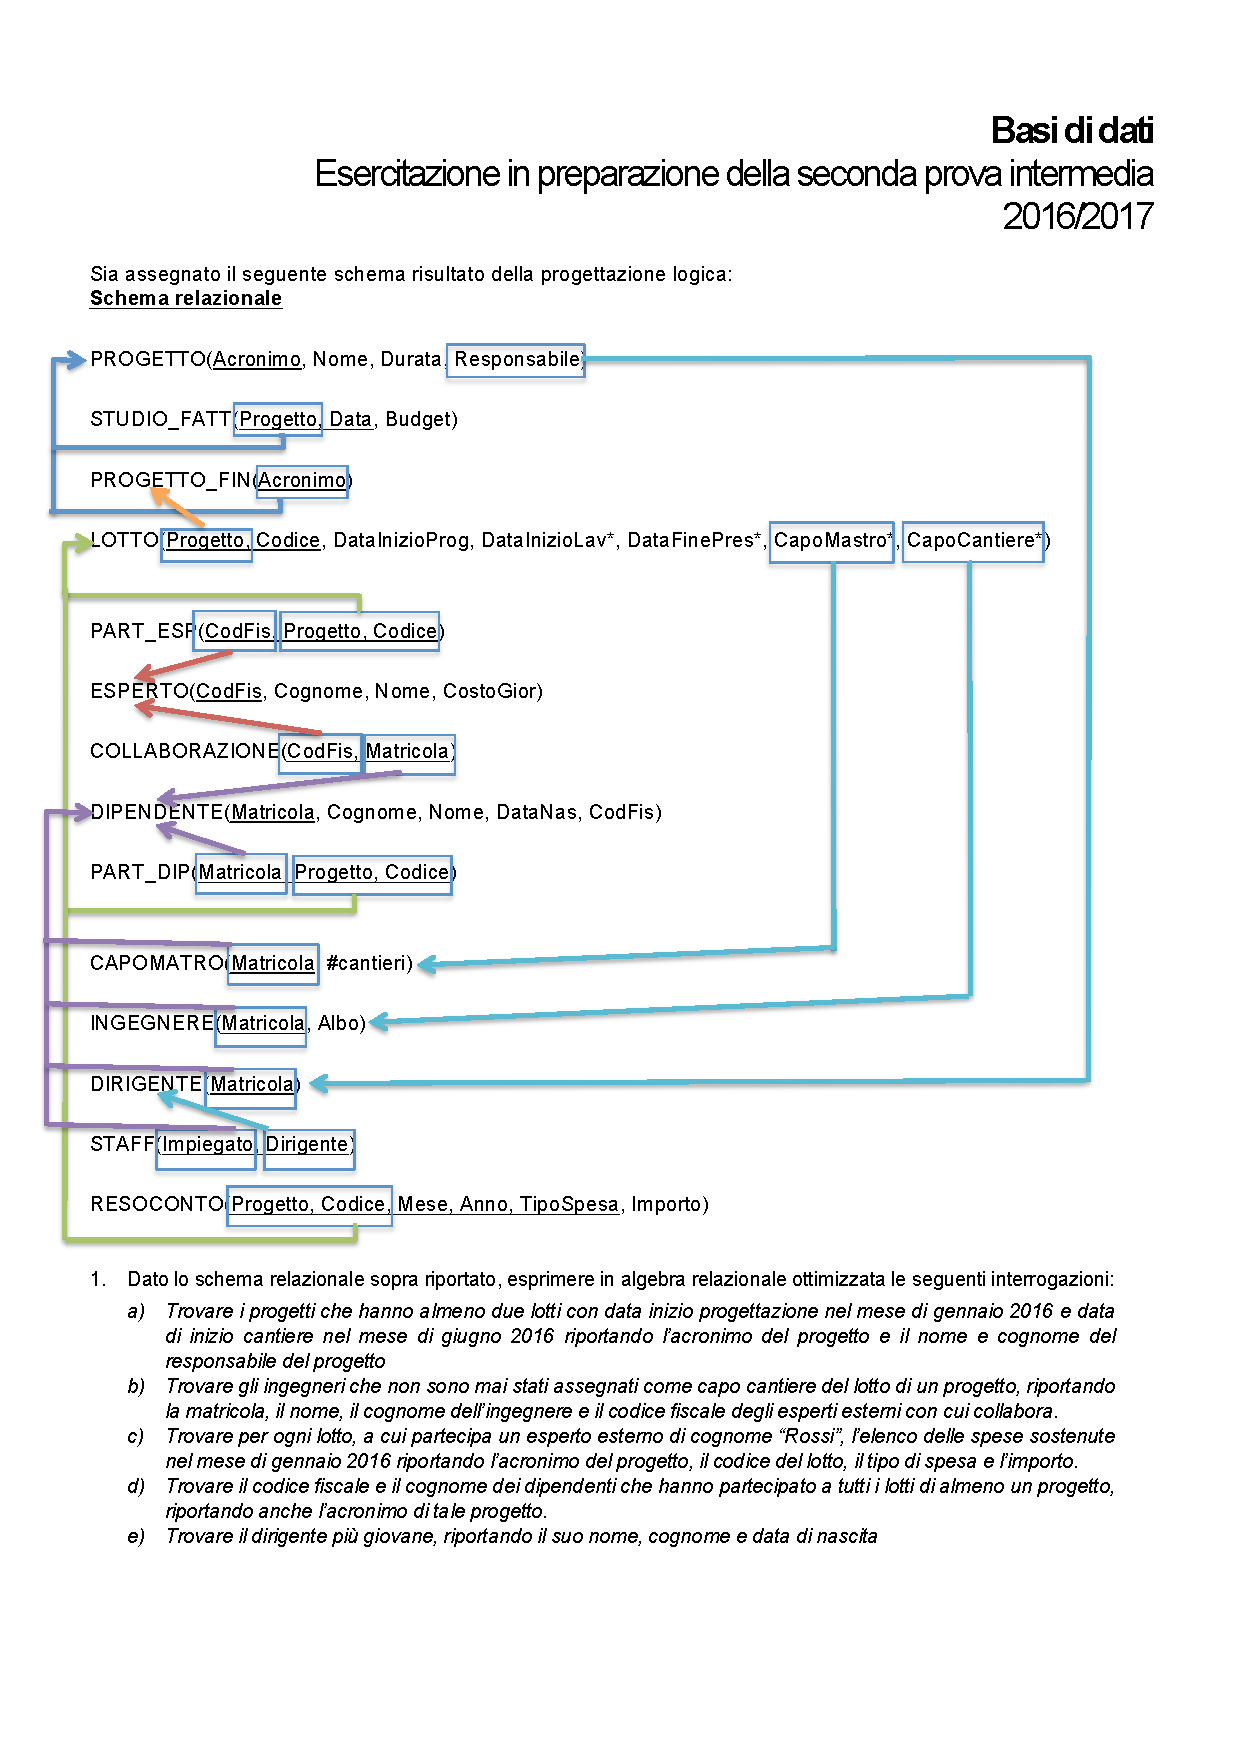
\includepdf[pages=-, offset=10 -10]{Esercitazione.pdf}
	
	\newpage
	\section{Soluzione dell'esercitazione}
		\subsection{Esercizio 1.a}
			\Tree [.$\Pi_{\textup{Acronimo, NomeR, CognomeR}}$
			 [.$\Join_S$ [.$\Join_R$ PROGETTO [.$\Join_G$ [.$\rho_{x\rightarrow \bar{x}}$ [.$\Pi_{\textup{Progetto, Codice}}$ [.$\sigma_P$ LOTTO ] ] ] [.$\Pi_{\textup{Progetto, Codice}}$ [.$\sigma_P$ LOTTO ] ] ] ] [.$\Pi_{\textup{Nome, Cognome}}$ [.DIPENDENTE ] ] ] ] 
	
		dove:
		\[
			S = \textup{Matricola, Nome, Cognome} \rightarrow \textup{Responsabile, NomeR, CognomeR}
		\]	
		\[
			R = \textup{Progetto}=\textup{Acronimo}
		\]
		\[
			G = \textup{Progetto}=\overline{\textup{Progetto}}\wedge \textup{Codice}\neq\overline{\textup{Codice}}
		\]
		\[
		P=
		\begin{cases}
			\textup{DataInizioProg} \geq \textup{'1/1/2016'} \\
			\textup{DataInizioProg} \leq \textup{'31/1/2016'} \\
			\textup{DataInizioLav} \geq \textup{'1/6/2016'} \\
			\textup{DataInizioLav} \leq \textup{'30/6/2016'} 
		\end{cases}			
		\]
		
		\subsection{Esercizio 1.b}
			\Tree [.$\Pi_{\textup{Matricola, Nome, Cognome, CodFis}}$ 
			[.$\Join$ [.$-$ [.$\Join$ INGEGNERE DIPENDENTE ] 
							[.$\Join_{\textup{CapoCantiere=Matricola}}$ [.$\Join$ INGEGNERE DIPENDENTE ] LOTTO ] ] 
					[.$\Pi_{\textup{CodFis}}$ COLLABORAZIONE ] ] ]
		
		\subsection{Esercizio 1.c}
			\Tree [.$\Pi_{\textup{Progetto, Codice, TipoSpesa, Importo}}$ 
			[.$\Join$ 
			[.$\Join$ [.$\Pi_{\textup{CF}}$ [.$\sigma_{\textup{Cognome}\neq\textup{'Rossi'}}$ ESPERTO ] ] PART\_ESP ] [.$\sigma_{\textup{Mese}=\textup{Gennaio}\wedge\textup{Anno}= 2016}$ RESOCONTO ] ] ]

		\subsection{Esercizio 1.d}
			\Tree[.$\Pi_{\textup{Cognome, Progetto, CodFisc}}$ 
			[.$\Join$ 
			[.$-$ [.$\Pi_{\textup{Matricola, Progetto}}$ [.PART\_DIP ] ] $r$ ] DIPENDENTE ] ]
			
			\bigskip
			
			Dove $r$ rappresenta tutte le tuple Matricola, Progetto di dipendenti che non hanno partecipato ad almeno uno dei lotti del progetto.
			
			\Tree [.$r$ [.$\Pi_{\textup{Matricola, Progetto}}$ [.$-$ [.$\Join$  [.$\Pi_{\textup{Matricola}}$ DIPENDENTE ] [.$\Pi_{\textup{Progetto, Codice}}$ LOTTO ] ] PART\_DIP ] ] ]
			
		\subsection{Esercizio 1.e}
			\Tree [.$\Pi_{\textup{Nome, Cognome, DataNasc}}$ [.$-$ [.$\Join$ DIRIGENTE DIPENDENTE ] 
			[.$\Pi_{\textup{Matricola, Cognome, Nome, DataNasc, CodFis}}$ [.$\Join_F$ 
				[.$\Join$ DIRIGENTE DIPENDENTE ] [.$\rho_{x \rightarrow \bar{x}}$ [.$\Join$ DIRIGENTE DIPENDENTE ] ] ] ] ]  ]
			
			\bigskip
			
			Dove
			\[
				F = \overline{\textup{DataNasc}} > \textup{DataNasc} \, \wedge \, \textup{Matricola} \neq \overline{\textup{Matricola}}
			\]
		
	\newpage
			
	\section{Concetto di vista}
	È una relazione derivata. Si specifica l'espressione che genera il suo
	contenuto. Esso quindi dipende dalle relazioni che compaiono
	nell'espressione.
	\begin{oss}
		Una vista può essere funzione di altre viste purché esista un
		ordinamento in grado di guidare il calcolo delle relazioni derivate.
	\end{oss}
	
	\subsection*{Vista virtuale}
	Una vista si dice  "virtuale" se viene calcolata ogni volta che serve.
	Conviene quando:
	\begin{itemize}
		\item L'aggiornamento è frequente
		\item L'interrogazione che genera la vista è semplice
	\end{itemize}
	Utilità delle viste:
	\begin{itemize}
		\item Consentono di personalizzare l'interfaccia utente
		\item Facilitano la gestione della privatezza dei dati
		\item Permettono di memorizzare nel DBMS interrogazioni complesse
		condivise
		\item Sono utili per rendere l'interfaccia delle applicazioni
		indipendente dallo schema logico (INDIPENDENZA LOGICA)
	\end{itemize}		
	
	\subsection*{Vista materializzata}
	Una vista si dice "materializzata" se viene calcolata e memorizzata
	esplicitamente nella base di dati.
	Conviene materializzare quando:
	\begin{itemize}
		\item L'aggiornamento è raro
		\item L'interrogazione che genera la vista è complessa
	\end{itemize}
	
	Se la vista viene materializzate è necessario ricalcolarne il
	contenuto ogni volta che le relazioni da cui dipende vengono
	aggiornate.
	
	\section{SQL - Structured Query Language}
		SQL è un linguaggio che è stato definito negli
		anni '70; è stato standardizzato negli anni '80 e '90 ed è oggi
		il linguaggio più diffuso per i DBMS relazionali. rappresenta uno strumento per l'interazione e la gestione della base di dati.
		È un linguaggio di \textbf{interrogazione dichiarativo}, cioè precisa le proprietà che devono essere rispettate dal risultato dell'interrogazione (query).
		Si basa sul calcolo relazionale e sulla logica del prim'ordine, in cui ogni espressione è dichiarativa e quindi definisce un insieme di proprietà.

		\subsection{Sintassi}
		\begin{lstlisting}
SELECT <Lista Attributi>
FROM <Lista Tabelle>
[ WHERE <Condizione> ]
		\end{lstlisting}
		La sua esecuzione produce una relazione risultato
		con le seguenti caratteristiche:
		\begin{itemize}
			\item \textbf{Schema}: è costituito da tutti gli attributi indicati in \lstinline|<ListaAttributi>|
			\item \textbf{Contenuto}: è costituito da tutte le tuple $t$ ottenute proiettando
			sugli attributi di \lstinline|<ListaAttributi>| (clausola\lstinline|SELECT|) le tuple $t'$
			appartenenti alle tabelle indicate in \lstinline|<ListaTabelle>| (clausola
			\lstinline|FROM|) che soddisfano l'eventuale condizione \lstinline|<Condizione>|
			(clausola \lstinline|WHERE|).
		\end{itemize}
		
		\newpage
		
		\subsection{Lista dei principali comandi}
		
		\begin{lstlisting}
SELECT DISTINCT <...> AS <alias> | * | 
	   COUNT (* | DISTINCT ... | ALL ...)
FROM <table/s> [AS] <alias>
[ WHERE <espr> ]
		\end{lstlisting}
	
		\subsection*{Clausola \lstinline|ORDER BY|}
		
		\begin{lstlisting}
ORDER BY <attr> [ASC | DESC] {, <attr> [ASC | DESC]}
		\end{lstlisting}
		
		\subsection*{Interrogazioni nidificate}
		\begin{lstlisting}
SELECT ...
FROM ...
WHERE <espr> <predicato> <ALL | ANY> (SELECT ... FROM ... WHERE)
		\end{lstlisting}
		dove predicato complesso è dell'insieme $\{ =, <>, <, >, <=, >= \}$ più \lstinline|ALL| o \lstinline|ANY|:
		\begin{itemize}
			\item A op ALL : questo predicato è soddisfatto dalla tupla $t$ se esiste almeno un
			valore $v$ nel risultato dell'interrogazione che
			verifica la condizione.
			
			\textbf{= ANY} si può scrivere \lstinline|IN|.
			\item A op ANY : questo predicato è soddisfatto dalla tupla $t$ se per ogni valore $v$
			nel risultato dell'interrogazione è verificata la
			condizione
			
			\textbf{<> ALL} si può scrivere \lstinline|NOT IN|.
		\end{itemize}
		
		\subsection*{Clausola \lstinline|EXISTS|}
		\begin{lstlisting}
SELECT ...
FROM ...
WHERE <espr> AND  <EXISTS | NOT EXISTS> (SELECT 1 FROM ... WHERE)
		\end{lstlisting}
		
		\subsection*{Operatori aggregati}
		\begin{lstlisting}
COUNT(* | [ DISTINCT | ALL ] <listaAttributi> )
SUM | MAX | MIN | AVG ([ DISTINCT | ALL ] <espressione>)
		\end{lstlisting}
		
		\subsection*{Clausola \lstinline|GROUP BY| e \lstinline|HAVING|}
		\begin{lstlisting}
SELECT <listaAttributi> FROM ... WHERE ...
GROUP BY <Attributo> {, <Attributo>}
HAVING <condizione_sel_gruppi>
ORDER BY ...
		\end{lstlisting}
		
		\subsection*{Interrogazioni insiemistiche}
		\begin{lstlisting}
<selectSQL> { UNION | INTERSECT | EXCEPT [all] <selectSQL> }
		\end{lstlisting}
		
		\subsection*{Viste}
		\begin{lstlisting}
CREATE VIEW <nomeVista> [(<lista attributi>)] AS <selectSQL>
		\end{lstlisting}
		\begin{itemize}
			\item Non è possibile definire viste ricorsive.
			\item È possibile definire una vista utilizzando altre viste,
			ma evitando dipendenze circolari (esempio di
			dipendenza circolare: V1 definita da V2 definita da
			V3 definita da V1).
			\item Le viste non sono in generale aggiornabili (solo in
			casi particolari i DBMS ammettono l'aggiornamento
			di viste).
		\end{itemize}
		
		\newpage
		
	\section{Transazioni}
	\underline{\textbf{Principale caratteristica di un DBMS}:} 
	
	\bigskip
	
	Un DBMS è un sistema transazionale, cioè fornisce un
	meccanismo per la definizione ed esecuzione di \textbf{transazioni}.
	
	\begin{defn}
		\textbf{Transazione:}
		È un'unità di lavoro svolto da un programma applicativo (che
		interagisce con una base di dati) per la quale si vogliono garantire
		alcune proprietà.
		
		Una transazione o va a buon fine e ha effetto sulla base di dati o
		abortisce e non ha nessun effetto sulla base di dati.
	\end{defn}
	
	\textbf{O tutto o niente!}
	
	\subsection{Sintassi}
	transazione:
		\begin{lstlisting}
begin transaction
<programma>
end transaction
		\end{lstlisting}
	programma:
		\begin{lstlisting}
<istruzione> | commit work | rollback work
{<istruzione> | commit work | rollback work}
		\end{lstlisting}
	
	La transazione va a buon fine all'esecuzione di un \lstinline|commit work|. Non ha
	invece effetto se viene eseguito un \lstinline|rollback work|.
	
	Una transazione è \textbf{ben formata} se:
	\begin{itemize}
		\item Inizia con un \lstinline|begin transaction|.
		\item Termina con un \lstinline|end transaction|.
		\item La sua esecuzione comporta il raggiungimento di un \lstinline|commit| o di un
		\lstinline|rollback work| e dopo il \lstinline|commit/rollback| non si eseguono altri
		accessi alla base di dati.
	\end{itemize}
	
	Esempio di transazione ben formata:
	\begin{lstlisting}
begin transaction;
	update CONTO set saldo = saldo - 1200
		where filiale = '005' and numero = 15;
	update CONTO set saldo = saldo + 1200
		where filiale = '005' and numero = 105;
commit work;
end transaction;
	\end{lstlisting}
	
	\subsection{Proprietà}
	
	Una transazione ha quattro proprietà:
	\begin{multicols}{2}
		\begin{enumerate}
			\item Atomicità
			\item Consistenza
			\item Isolamento
			\item Persistenza
		\end{enumerate}
		
		\columnbreak
		
		\begin{itemize}
			\item[] \textbf{A}tomicity
			\item[] \textbf{C}onsistency
			\item[] \textbf{I}solation
			\item[] \textbf{D}urability
		\end{itemize}
	\end{multicols}
	Un DBMS che gestisce transazioni dovrebbe
	garantire per ogni transazione che esegue tutte
	queste proprietà.
	
	\newpage
	
	\subsection{Atomicità}
	Una transazione è una unità di esecuzione \textbf{indivisibile}. O viene
	eseguita completamente o non viene eseguita affatto.
	
	Implicazioni:
	\begin{itemize}
		\item Se una transazione viene interrotta prima del commit, il lavoro fin
		qui eseguito dalla transazione deve essere disfatto ripristinando la
		situazione in cui si trovava la base di dati prima dell'inizio della
		transazione.
		\item Se una transazione viene interrotta all'esecuzione del commit
		(commit eseguito con successo), il sistema deve assicurare che la
		transazione abbia effetto sulla base di dati.
	\end{itemize}
	
	\subsection{Consistenza}
	L'esecuzione di una transazione non deve violare i vincoli di integrità.
	
	Implicazioni:
	Al verificarsi della violazione di un vincolo il sistema può:
	\begin{itemize}
		\item \textbf{verifica immediata}:
		
			Viene abortita l'ultima operazione e il sistema restituisce
			all'applicazione una segnalazione d'errore
			L'applicazione può quindi reagire alla violazione.
		\item \textbf{verifica differita}:
		
			Al commit se un vincolo di integrità viene violato la transazione
			viene abortita senza possibilità da parte dell'applicazione di
			reagire alla violazione.
	\end{itemize}
	
	\subsection{Isolamento}
	L'esecuzione di una transazione deve essere \textbf{indipendente} dalla
	contemporanea esecuzione di altre transazioni.
	
	Implicazioni:
	\begin{itemize}
		\item Il rollback di una transazione non deve creare rollback a catena di
		altre transazioni che si trovano in esecuzione contemporaneamente.
		\item Il sistema deve regolare l'esecuzione concorrente
	\end{itemize}
	
	\subsection{Persistenza}
	L'effetto di una transazione che ha eseguito il commit non deve andare
	perso.
	
	Implicazioni:
	\begin{itemize}
		\item Il sistema deve essere in grado, in caso di guasto, di garantire gli
		effetti delle transazioni che al momento del guasto avevano già
		eseguito un commit.
	\end{itemize}

\newpage
		
	\section{Architettura di un DBMS}
	L'architettura mostra i moduli principali che
	possiamo individuare nei DBMS attuali, considerando
	le diverse funzionalità che il DBMS svolge durante
	l'esecuzione delle transazioni.
	Per ogni modulo dell'architettura presentiamo le
	funzionalità che esso svolge e alcune delle tecniche che
	applica.
	
	\bigskip
	
	\begin{center}
		\begin{tikzpicture}[>=latex,scale=0.9]
		\draw[color=gray!60!] (-9,-7) rectangle (4,9);
		\node at (3,8) {\textbf{DBMS}};
		\node (tran) at (-2.5,10) {$\textup{Transazione}_1, \dots, \textup{Transazione}_n$};
		\draw[->] (-3,9.75) -- (-2.5,9);
		\draw[->] (-2, 9.75) -- (-2.5,9);
		\node (a) at (-2.5, 7) [entità,align=center] {Ottimizzatore\\ di\\ Espressioni DML};
		\node (b) at (-2.5, 5) [align=center] {Piano di Esecuzione};
		\node (c) at (-2.5, 3.5) [entità,align=center] {Gestore dei\\ Metodi d'accesso};
		\node (d) at (-2.5, 1.5) [align=center] {Richieste di\\ Pagine dati e\\ Pagine Indice};
		\node (e) at (-2.5, -0.5) [entità,align=center] {Gestore\\ dell'affidabilità};
		\node (e-side) at (e.east) [draw,right,font=\footnotesize,yshift=0.25cm] {ATOMICITÀ};
		\node (e-side2) at (e-side.south) [draw,below,font=\footnotesize,xshift=0.2cm] {PERSISTENZA};
		\node (f) at (-2.5, -3) [align=center] {Richieste di\\ Pagine dati,\\ Pagine Indice e\\ Pagine del Log};
		\node (g) at (-2.5, -5.5) [entità,align=center] {Gestore del buffer};
		\node (g-side) at (g.east) [draw,right,font=\footnotesize,yshift=0.25cm] {ATOMICITÀ};
		\node (g-side2) at (g-side.south) [draw,below,font=\footnotesize,xshift=0.2cm] {PERSISTENZA};
		\node (h) at (2, 3.5) [entità,align=center] {Gestore della\\ Concorrenza};
		\node (h-below) at (h.south) [draw, below, font=\footnotesize] {ATOMICITÀ};
		\node (h-below2) at (h-below.south) [draw, below, font=\footnotesize] {ISOLAMENTO};
		\draw[->] (-2.5, 9) -- (a.north);
		\draw[->] (a.south) -- (b.north) node[midway, right, font=\footnotesize] {produce}; 
		\draw[->] (b.south) -- (c.north) node[midway, right, font=\footnotesize] {viene eseguito da}; 
		\draw[->] (c.south) -- (d.north) node[midway, right, font=\footnotesize] {produce}; 
		\draw[->] (d.south) -- (e.north); 
		\draw[->] (e.south) -- (f.north) node[midway, right, font=\footnotesize] {produce}; 
		\draw[->] (f.south) -- (g.north);
		\draw[<->] (c.east) -- (h.west);
		\draw[<->] (g.south) -- (-2.5, -7.5);
		
		\path (-2.5,-10) pic {disc bottom} (-2.5,-8.75) pic {disc};
		\node at (-2.5, -7.75) {Memoria Secondaria};
		\node at (-2.5, -9.65) [align=center] {Base di\\Dati};
		\node at (-2.5, -10.8) {Log};
		\end{tikzpicture}
	\end{center}
	
	\section{Strutture fisiche e di accesso ai dati}
	
	Le basi di dati gestite da un DBMS risiedono in
	memoria secondaria, in quanto sono:
	\begin{itemize}
		\item Grandi: non possono essere contenute in memoria centrale
		\item Persistenti: hanno un tempo di vita che non è limitato
		all'esecuzione dei programmi che le utilizzano
	\end{itemize}
	Caratteristiche della memoria secondaria:
	\begin{itemize}
		\item Non è direttamente utilizzabile dai programmi
		\item I dati sono organizzati in blocchi (o pagine)
		\item Le uniche operazioni possibili sono la lettura e la scrittura di
		un intero blocco (pagina)
		\item Il costo di tali operazioni è ordini di grandezza maggiore del
		costo per accedere ai dati in memoria centrale
	\end{itemize}
	
	\subsection{Gestore del buffer}
		L'interazione tra memoria secondaria e memoria
		centrale avviene attraverso il trasferimento di pagine
		della memoria secondaria in una zona appositamente
		dedicata della memoria centrale detta \textbf{buffer}.
		
		Si noti che:
		\begin{itemize}
			\item Il buffer è una zona di memoria condivisa
			dalle applicazioni
			\item Quando uno stesso	dato viene utilizzato più volte in tempi
			ravvicinati il buffer evita l'accesso alla memoria secondaria
			\item La gestione ottimale del buffer è strategica
			per ottenere buone prestazioni nell'accesso ai dati
		\end{itemize}
		\begin{center}
			\begin{tikzpicture}[x=\daywidth, y=-1cm, node distance=0cm, outer sep = 0pt, scale=0.6, every node/.style={scale=0.6}, >=latex]
			\tikzstyle{cell}=[rectangle,draw, minimum width=\daywidth,,minimum height=1cm,
			anchor=north west,text centered,text width=5 em]
			
			\foreach \x in {1, 2, ..., 6}{
				\foreach \y in {1, 2, ..., 6}{
					\node[cell, pattern=north west lines, pattern color=gray!80!white] at (\x,\y) {\huge \textbf{L}};
				}	
			}
			
			\node[cell, fill=white] at (1,1) {\huge $\mathbf{B_{2,0}}$};
			\node[cell, fill=white] at (4,1) {\huge $\mathbf{B_{1,1}}$};
			\node[cell, fill=white] at (1,2) {\huge $\mathbf{B_{1,1}}$};
			\node[cell, fill=white] at (2,2) {\huge $\mathbf{B_{1,1}}$};
			\node[cell, fill=white] at (3,2) {\huge $\mathbf{B_{1,1}}$};
			\node[cell, fill=white] at (4,1) {\huge $\mathbf{B_{1,0}}$};
			\node[cell, fill=white] at (3,3) {\huge $\mathbf{B_{1,0}}$};
			\node[cell, fill=white] at (5,3) {\huge $\mathbf{B_{0,0}}$};
			\node[cell, fill=white] at (6,3) {\huge $\mathbf{B_{0,0}}$};
			\node[cell, fill=white] at (5,4) {\huge $\mathbf{B_{0,0}}$};
			\node[cell, fill=white] at (4,5) {\huge $\mathbf{B_{0,0}}$};
			\node[cell, fill=white] at (5,5) {\huge $\mathbf{B_{0,0}}$};
			
			\draw[ultra thick,<->] (4,7.5) -- (4,9);
			
			\path (4,10) pic[rotate=180] {disc} ;
			\node at (4,12) {\Large Memoria secondaria};
			\end{tikzpicture}
		\end{center}
	
		$B_{i,j}$ indica che nella pagina del buffer è caricato il blocco
		$B$, inoltre $ i $ indica che il blocco è attualmente utilizzato da $i$ transazioni mentre $j$ è $1$ se il blocco è stato modificato e $0$ altrimenti. 
		
		\textbf{L} indica pagina libera.
		
		Il buffer è organizzato in \textbf{pagine}. Una pagina ha le dimensioni di un blocco della memoria secondaria.
		Il gestore del buffer si occupa del caricamento/salvataggio delle pagine in memoria secondaria.
		
		\textbf{Politica} del gestore dei buffer:
		\begin{itemize}
			\item In caso di richiesta di lettura di un blocco, se il blocco è presente in una pagina del buffer allora non si esegue una lettura su memoria secondaria e si restituisce un puntatore alla
			pagina del buffer, altrimenti si cerca una pagina libera e si carica il blocco nella pagina, restituendo il puntatore alla pagina stessa.
			\item In caso di richiesta di scrittura di un blocco precedentemente
			caricato in una pagina del buffer, il gestore del buffer può
			decidere di differire la scrittura su memoria secondaria in un
			secondo momento.
		\end{itemize}
		
		In entrambi i casi (lettura e scrittura) l'obiettivo e quello di
		aumentare la velocità di accesso ai dati.
		Tale comportamento del gestore dei buffer si basa sul \textbf{principio di
		località}: 
		\begin{quotation}
			\textit{"I dati referenziati di recente hanno maggiore probabilità di
			essere referenziati nuovamente in futuro ".}
		\end{quotation}	
		Inoltre, una nota legge	empirica dice che: "il $20\%$ dei dati è acceduto dall'$80\%$ delle applicazioni".
		Tutto ciò rende conveniente dilazionare la scrittura su memoria
		secondaria delle pagine del buffer.
		
		\subsection{Gestione delle pagine}
		Dati necessari per la gestione delle pagine:
		\begin{itemize}
			\item Per ogni pagina del buffer si memorizza il blocco contenuto
			indicando il file e il numero di blocco (o offset)
			\item Per ogni pagina del buffer si memorizza un insieme di variabili
			di stato tra cui si trovano sicuramente:
				\subitem{-} Un
				contatore per indicare il numero di transazioni che utilizzano le
				pagine
				\subitem{-} Un bit di stato per indicare se la pagina è stata modificata o no.
		\end{itemize}
		Primitive per la gestione delle pagine:
		\begin{itemize}
			\item \textbf{Fix}: viene usata dalle transazioni per richiedere l'accesso ad un
			blocco e restituisce al chiamante un puntatore alla pagina contenente
			il blocco richiesto. Passi della primitiva:
				\subitem{-} Il blocco richiesto viene cercato nelle pagine del buffer, in caso sia
				presente, si restituisce un puntatore alla pagina contenente il blocco
				\subitem{-} Altrimenti, viene scelta una pagina libera P (contatore = zero). Si sceglie la
				pagina in base a criteri diversi: la pagina usata meno di recente (LRU) o
				caricata da più tempo (FIFO). Se il bit di stato di P è a 1 P viene salvata in
				memoria secondaria (operazione di flush). Si carica il blocco in P
				aggiornando file e numero di blocco corrispondenti.
				\subitem{-} Se non esistono pagine libere, il gestore del buffer può adottare due
				politiche (STEAL): "ruba" una pagina ad un'altra transazione (operazione
				di flush); oppure (NO STEAL) sospende la transazione inserendola in una
				coda di attesa. Se una pagina si libera (contatore = zero) il gestore si
				comporterà come al punto precedente.
				\subitem{-} Quando una transazione accede ad una pagina per la prima volta il
				contatore si incrementa.
			\item \textbf{unfix}: viene usata dalle transazione per indicare che la transazione ha
			terminato di usare il blocco. L’effetto è il decremento del contatore di utilizzo della pagina.
			\item \textbf{setDirty}: viene usata dalle transazioni per indicare al gestore del
			buffer che il blocco della pagina è stato modificato: L'effetto è la modifica del bit di stato a $1$
			\item \textbf{force}: viene usata per salvare in memoria secondaria in modo
			\textbf{sincrono} il blocco contenuto nella pagina (primitiva usata dal
			gestore dell'affidabilità). L'effetto è il salvataggio in memoria secondaria del blocco e il bit di stato posto a zero.
			\item \textbf{flush}: viene usata dal gestore del buffer per salvare blocchi sulla
			memoria secondaria in modo \textbf{asincrono}. Tale operazione libera
			pagine "dirty".
		\end{itemize}
		
	\begin{tikzpicture}[>=latex]
		\node[entità] at (3,2) {Gestore dell'affidabilità};
		\node[entità,align=center,baseline=0.4cm] (a) at (1,0) {\hspace*{0.5cm} Gestore del buffer \hspace*{0.5cm}
			\tikz[scale=0.7]{\draw[help lines,xstep=2,ystep=0.5] (4,0) grid (10,1.5)}};
		\draw[->] (-2.5,1.5) -- (-2.5,0.7) node[midway, left] {flush};
		\draw[->] (1.4,1.5) -- (1.4,0.7) node[midway, left] {force};
		\draw[->] (2,1.5) -- (2,0.7) node[midway, left] {fix};
		\draw[->] (3,1.5) -- (3,0.7) node[midway, left] {unfix};
		\draw[->] (4.5,1.5) -- (4.5,0.7) node[midway, left] {setDirty};
		\draw[<->] (a.east) -- (6,0);
		\path (7.25,0.5) pic {disc} ;
		\node at (7.25,1.25) {Memoria Secondaria};
	\end{tikzpicture}
	
	\subsection{Gestore dell'affidabilità}
	È il modulo responsabile di ciò che riguarda:
	\begin{itemize}
		\item L'esecuzione delle istruzioni per la gestione delle
		transazioni
		\item La realizzazione delle operazioni necessarie al ripristino
		della base di dati dopo eventuali malfunzionamenti
	\end{itemize}
	Per il suo funzionamento il gestore dell'affidabilità
	deve disporre di un dispositivo di \textbf{memoria
	stabile}.
	\textbf{memoria stabile} = memoria \textbf{resistente ai guasti}
	
	In memoria stabile viene memorizzato il file di \textbf{log}
	che registra in modo sequenziale le operazioni eseguite
	dalle transazioni sulla base di dati.
	
	\subsection*{Record di log di transizione}
	\begin{itemize}
		\item Begin della transazione T: record B(T)
		\item Commit della transazione T: record C(T)
		\item Abort della transazione T: record A(T)
		\item Insert, Delete e Update eseguiti dalla transazione T sull'oggetto O:
			\subitem record I(T,O,AS): AS=After State
			\subitem record D(T,O,BS): BS=Before State
			\subitem record U(T,O,BS,AS)
	\end{itemize}
	
	I record di transazione salvati nel LOG consentono di eseguire in caso di
	ripristino le seguenti operazioni:
	\begin{itemize}
		\item \textbf{undo}: per disfare un'azione su un oggetto O è sufficiente ricopiare in
		O il valore BS; l'insert/delete viene disfatto cancellando/inserendo O;
		\item \textbf{redo}: per rifare un'azione su un oggetto O è sufficiente ricopiare in O
		il valore AS; l'insert/delete rifatto inserendo/cancellando O;
	\end{itemize}
	
	Gli inserimenti controllano sempre l'esistenza di O (non si inseriscono
	duplicati).
	
	Proprietà di \textbf{idempotenza}:
	\begin{itemize}
		\item{} UNDO(UNDO(A))=UNDO(A)
		\item{} REDO(REDO(A))=REDO(A)
	\end{itemize}
	
	\subsection*{Record di log di sistema}
	\begin{itemize}
		\item Operazione di \textbf{dump} della base di dati: \textbf{record di DUMP.}
		Contiene un riepilogo della struttura delle tabelle del database medesimo e/o i relativi dati, ed è normalmente nella forma di una lista di dichiarazioni SQL. Tale dump è usato per lo più per fare il backup del database, poiché i suoi contenuti possono essere ripristinati nel caso di perdita di dati. I database "corrotti" (ossia, i cui dati non sono più utilizzabili in seguito ad una modifica "distruttiva" di qualche parametro di formato) possono spesso essere rigenerati mediante l'analisi del dump. I dumps di database sono spesso pubblicati dai progetti di software libero o di contenuto libero, in modo tale da consentire il riutilizzo o il forking dei database cui si riferiscono.
		Con l'espressione \textit{core dump} s'intende specificamente lo stato registrato della memoria di un programma in un determinato momento, specie quando tale programma si sia chiuso "inaspettatamente" (crash).
		
		\item Operazione di \textbf{CheckPoint}: record $CK(T_1, \dots, T_n)$ indica che	all'esecuzione del CheckPoint le transazioni attive erano 
		$T_1, \dots, T_n$.
	\end{itemize}
	
	L'operazione di CheckPoint: è un'operazione svolta
	periodicamente dal gestore dell'affidabilita; prevede i
	seguenti passi:
	\begin{itemize}
		\item Sospensione delle operazioni di scrittura, commit e abort delle
		transazioni.
		\item Esecuzione di operazione di force sulle pagine "dirty" di
		transazioni che hanno eseguito il commit.
		\item Scrittura sincrona sul file di LOG del record di CheckPoint con
		gli identificatori delle transazioni attive.
		\item Ripresa delle operazioni di scrittura, commit e abort delle
		transazioni.
	\end{itemize}
	Regole per la scrittura sul LOG ed esecuzione delle
	transazioni:
	\begin{itemize}
		\item Regola \textbf{WAL} (Write Ahead Log): i record di log devono essere
		scritti sul LOG prima dell'esecuzione delle corrispondenti
		operazioni sulla base di dati (garantisce la possibilità di fare
		sempre UNDO).
		\item Regola \textbf{Commit-Precedenza}: i record di log devono essere
		scritti sul LOG prima dell'esecuzione del COMMIT della
		transazione (garantisce la possibilità di fare sempre REDO)
	\end{itemize}
	Tali regole consentono di salvare i blocchi delle pagine
	"dirty" in modo totalmente asincrono rispetto al
	commit delle transazioni.
	
	\subsection*{Esecuzione del commit di una transazione}
		Una transazione sceglie in \textbf{modo atomico} l'esito di COMMIT nel
		momento in cui scrive nel file di LOG in modo \textbf{sincrono} (primitiva
		\textbf{force}) il suo record di COMMIT.
	
	\subsection*{Operazioni di ripristino in caso di guasto}
	Tipi di guasto:
	\begin{itemize}
		\item \textbf{Guasto di sistema}: perdita del contenuto della
		memoria centrale $\quad \rightarrow \quad$ \textbf{Ripresa a caldo}.
		\item \textbf{Guasto di dispositivo}: perdita di parte o tutto il
		contenuto della base di dati in memoria secondaria 
		$\quad \rightarrow \quad$ \textbf{Ripresa a freddo}.
	\end{itemize}
	Modello di funzionamento:
	
	\vspace*{1cm}
	
	\begin{tikzpicture}[>=latex, scale = 1.2, every node/.style={scale=1.2}]
		\node[cerchio, align=center] (normale) at (1,1) {Funzionamento\\normale};
		\node[cerchio] (stop) at (5,1) {STOP};
		\node[cerchio] (ripristino) at (2.5, -1) {RIPRISTINO};
		
		\draw[bend left, ->] (normale) to node[above] {Fail} (stop);
		\draw[bend left, ->] (stop) to node[right] {Boot} (ripristino.east);
		\draw[bend left, ->] (ripristino.west) to node[below left, align=center] {Fine\\Ripristino} (normale);
		\draw[bend left, ->] (ripristino) to node[below right] {Fail} (stop);
	\end{tikzpicture}
	
	\subsection*{Ripresa a caldo}
	Passi:
	\begin{itemize}
		\item Si accede all'ultimo blocco del LOG e si ripercorre all'indietro il log fino
		al più recente record CK.
		\item Si decidono le transazioni da rifare/disfare inizializzando l'insieme
		UNDO con le transazioni attive al CK e l'insieme REDO con l'insieme
		vuoto.
		\item Si ripercorre in avanti il LOG e per ogni record B(T) incontrato si
		aggiunge T a UNDO e per ogni record C(T) incontrato si sposta T da
		UNDO a REDO.
		\item Si ripercorre all'indietro il LOG disfacendo le operazioni eseguite dalle
		transazioni in UNDO risalendo fino alla prima azione della transazione più vecchia.
		\item Si rifanno le operazioni delle transazioni dell'insieme REDO.
	\end{itemize}
	
	\subsection*{Esercizio}
	\begin{lstlisting}
B(T1), B(T2), U(T2,O1,B1,A1), I(T1,O2,A2), B(T3),
C(T1), B(T4), U(T3,O2,B3,A3), U(T4,03,B4,A4),
CK(T2,T3,T4), C(T4), B(T5), U(T3,O3,B5,A5),
U(T5,O4,B6,A6), D(T3,O5,B7), A(T3), C(T5),
I(T2,O6,A8) guasto
	\end{lstlisting}
Che passi svolge la ripresa a caldo?

\bigskip

	\begin{multicols}{3}
		\begin{tabular}{cc}
			undo & redo \\
			\midrule
			$T_2$ & \\
			$T_3$ & \\
			$\cancel{T_4}$ & $ T_4 $ \\
			$\cancel{T_5}$ & $ T_5 $
		\end{tabular}
		
		\columnbreak
		
		Undo:
		\begin{itemize}
			\item \lstinline|Delete(06)|
			\item \lstinline|Insert(05)|
			\item \lstinline|O3 := B5;|
			\item \lstinline|O2 := B3;|
			\item \lstinline|O1 := B1;|
		\end{itemize}	
		
		\columnbreak 
		
		Redo:
		\begin{itemize}
			\item \lstinline|O3 := A4;|
			\item \lstinline|O4 := A6;|
		\end{itemize}
	\end{multicols}
	
	\newpage

	\subsection*{Ripresa a freddo}
	Passi:
	\begin{itemize}
		\item Si accede al DUMP della base di dati e si ricopia
		selettivamente la parte deteriorata della base di dati.
		\item Si accede al LOG risalendo al record di DUMP.
		\item Si ripercorre in avanti il LOG rieseguendo tutte le
		operazioni relative alla parte deteriorata comprese le
		azioni di commit e abort.
		\item Si applica una ripresa a caldo.
	\end{itemize}
	
	\subsection{Gestore dei metodi di accesso}
	È il modulo del DBMS che esegue il piano di
	esecuzione prodotto dall'ottimizzatore e produce
	sequenze di accessi alle pagine della base di dati
	presenti in memoria secondaria.
	
	\vspace*{0.5cm}
	\begin{center}
		\begin{tikzpicture}[>=latex]
		\node (a) at (0,2) {piano di esecuzione};
		\node[entità, align=center] (b) at (0,0) {Gestore dei metodi\\ d'accesso};
		\node[align=center] (c) at (0,-2) {Richiesta di accesso alle\\pagine Dati/Indici (fix,\\unfix, setDirty)};
		\draw[->] (a) -- (b);
		\draw[->] (b) -- (c);
		\end{tikzpicture}
	\end{center}
	
	\subsection*{Metodi d'accesso}
	Sono i moduli software che implementano gli algoritmi
	di accesso e manipolazione dei dati organizzati in
	specifiche strutture fisiche.
	
	Esempio:
	\begin{itemize}
		\item Scansione sequenziale
		\item Accesso via indice
		\item Ordinamento
		\item Varie implementazioni del join
	\end{itemize}
	\noindent
	Ogni metodo d'accesso ai dati conosce:
	\begin{itemize}
		\item L'organizzazione delle \textbf{tuple} nelle pagine DATI salvate in
		memoria secondaria (\ul{come una tabella viene organizzata
		in pagine DATI} della memoria secondaria)
		\item L'organizzazione fisica delle \textbf{pagine} DATI contenenti tuple
		e delle pagine che memorizzano le strutture fisiche di
		accesso o INDICI (\ul{come le tuple o i record dell'indice
		vengono memorizzati all'interno delle pagine}).
	\end{itemize}
	\noindent
	In una pagina DATI sono presenti informazioni utili e
	informazioni di controllo:
	\begin{itemize}
		\item Informazioni utili: tuple della tabella
		\item Informazioni di controllo: dizionario, bit di parità, altre
		informazioni del file system o del metodo d'accesso specifico.
	\end{itemize}
	
	\subsection*{Struttura della pagina dati}
	
	\vspace{0.5cm}
	
	\begin{tikzpicture}[>=latex]
		\fill[brown!50] (0,0) rectangle (1,3);
		\fill[gray!50] (1,0) rectangle (2,3);
		\fill[yellow!80] (2,0) rectangle (4.2,3);
		\fill[red!50] (4.2,0) rectangle (7.4,3);
		\fill[blue!50] (7.4,0) rectangle (10.2,3);
		\fill[red!50] (10.2,0) rectangle (10.4,3);
		\fill[red] (10.4,0) rectangle (10.8,3);
		\fill[gray!50] (10.8,0) rectangle (11.8,3);
		\fill[brown!50] (11.8,0) rectangle (12.8,3);
		
		\draw (1,3) -- (1,0);
		\draw (2,3) -- (2,0);
		\foreach \x in {2.2, 2.4, ..., 4.2}{
			\draw (\x,3) -- (\x,0);
		}
		\foreach \x in {7.4, 7.8, ..., 10.4}{
			\draw (\x,3) -- (\x,0);
		}
		\draw (10.4,0) -- (10.4,3);
		\draw (10.8,0) -- (10.8,3);
		\draw (11.8,3) -- (11.8,0);
		
		\draw (0,3) -- (12.8,3) -- (12.8,0) -- (0,0) -- cycle;
		
		\draw (1.5,-1) -- (11.25,-1) node[midway,above] {Informazioni di controllo del metodo d'accesso};
		\draw[->] (1.5,-1) -- (1.5,0);
		\draw[->] (11.25,-1) -- (11.25,0);
		
		\draw (0.5,-2) -- (12.25,-2) node[midway,above] {Informazioni di controllo del File System};
		\draw[->] (0.5,-2) -- (0.5,0);
		\draw[->] (12.25,-2) -- (12.25,0);
		
		\draw[->] (3,3.5) node[above] {dizionario delle tuple} -- (3.5,3);
		
		\draw[->] (8,3.5) node[above] {tuple} -- (8.5,3);
		
		\draw[->] (11,3.5) node[above] {bit di parità} -- (10.6,3);
	\end{tikzpicture}
	
	\subsection*{Struttura del dizionario}
	\begin{itemize}
		\item \textbf{Tuple di lunghezza fissa}: il dizionario non è necessario, si
		deve solo memorizzare la dimensione delle tuple e l'offset
		del punto iniziale
		\item \textbf{Tuple di lunghezza variabile}: il dizionario memorizza
		l'offset di ogni tupla presente nella pagina e di ogni
		attributo di ogni tupla
	\end{itemize}
	\textbf{Lunghezza massima di una tupla} = dimensione massima
	dell'area disponibile su una pagina, altrimenti va gestito il
	caso di tuple memorizzate su più pagine (in postgreSQL si
	veda la soluzione TOAST - The Oversized-Attribute Storage
	Technique).
	
	\subsection*{Operazioni}
	\begin{itemize}
		\item Inserimento di una tupla
			\subitem Se esiste spazio contiguo sufficiente: inserimento semplice
			\subitem Se non esiste spazio contiguo ma esiste spazio sufficiente:
			riorganizzare lo spazio ed eseguire un inserimento semplice
			\subitem Se non esiste spazio sufficiente: operazione rifiutata
		\item Cancellazione: sempre possibile anche senza riorganizzare
		\item Accesso ad una tupla
		\item Accesso ad un attributo di una tupla
		\item Accesso sequenziale (di solito in ordine di chiave primaria)
		\item Riorganizzazione
	\end{itemize}
	
	\subsection*{Rappresentazione di una tabella a livello fisico}

	\begin{multicols}{3}
		\subsection*{Livello fisico}
		(memoria secondaria)
		
		\begin{tikzpicture}[>=latex, scale=0.2,every node/.style={scale=1.1}]
			
			\fill[yellow!80] (2,0) rectangle (4.2,3);
			\fill[red!50] (4.2,0) rectangle (7.4,3);
			\fill[blue!50] (7.4,0) rectangle (10.2,3);
			
			\foreach \x in {2.2, 2.4, ..., 4.2}{
				\draw (\x,3) -- (\x,0);
			}
			\foreach \x in {7.4, 7.8, ..., 10.4}{
				\draw (\x,3) -- (\x,0);
			}
			
			\draw (2,3) -- (10.2,3) -- (10.2,0) -- (2,0) -- cycle;
		\end{tikzpicture}
		\hspace{0.5cm}
		\begin{tikzpicture}[>=latex, scale=0.2,every node/.style={scale=1.1}]
		
			\fill[yellow!80] (2,0) rectangle (4.2,3);
			\fill[red!50] (4.2,0) rectangle (7.4,3);
			\fill[blue!50] (7.4,0) rectangle (10.2,3);
			
			\foreach \x in {2.2, 2.4, ..., 4.2}{
				\draw (\x,3) -- (\x,0);
			}
			\foreach \x in {7.4, 7.8, ..., 10.4}{
				\draw (\x,3) -- (\x,0);
			}
			
			\draw (2,3) -- (10.2,3) -- (10.2,0) -- (2,0) -- cycle;
		\end{tikzpicture}

		\begin{flushright}
			\begin{tikzpicture}[>=latex, scale=0.2,every node/.style={scale=1.1}]
			
			\fill[yellow!80] (2,0) rectangle (4.2,3);
			\fill[red!50] (4.2,0) rectangle (7.4,3);
			\fill[blue!50] (7.4,0) rectangle (10.2,3);
			
			\foreach \x in {2.2, 2.4, ..., 4.2}{
				\draw (\x,3) -- (\x,0);
			}
			\foreach \x in {7.4, 7.8, ..., 10.4}{
				\draw (\x,3) -- (\x,0);
			}
			
			\draw (2,3) -- (10.2,3) -- (10.2,0) -- (2,0) -- cycle;
			\end{tikzpicture}

			
			\begin{tikzpicture}[>=latex, scale=0.2,every node/.style={scale=1.1}]
			
			\fill[yellow!80] (2,0) rectangle (4.2,3);
			\fill[red!50] (4.2,0) rectangle (7.4,3);
			\fill[blue!50] (7.4,0) rectangle (10.2,3);
			
			\foreach \x in {2.2, 2.4, ..., 4.2}{
				\draw (\x,3) -- (\x,0);
			}
			\foreach \x in {7.4, 7.8, ..., 10.4}{
				\draw (\x,3) -- (\x,0);
			}
			
			\draw (2,3) -- (10.2,3) -- (10.2,0) -- (2,0) -- cycle;
			\end{tikzpicture}
		\end{flushright}

		\columnbreak
		
		Struttura fisica:
		\begin{itemize}
			\item Strutture ad accesso calc.
			\item Seriale
			\item Array
			\item Sequenza ordinata o file sequenziale
		\end{itemize}
		
		
		\begin{tikzpicture}[>=latex]
			\draw[help lines, xstep=0.5,ystep=0.5] (0,0) grid (2,2); 
			\draw[<->] (-0.5,1.5) -- (-1,1.5);
			\draw[<->] (-0.5,0.5) -- (-1,0.5);
			\draw[thick] (-0.25,1) -- (2.25,1);
			\draw[->] (2,1.75) to [out=0,in=360,looseness=3] (2,1.25);
			\draw[->] (2,1.25) to [out=0,in=360,looseness=3] (2,0.75);
			\draw[->] (2,0.75) to [out=0,in=360,looseness=3] (2,0.25);
			\draw[fill=yellow] (2.75,2) -- (4,1) -- (2.75,0) -- cycle;
			\node at (3.25,1) {Indice};
		\end{tikzpicture}
		
		\columnbreak
		
		\subsection*{Livello logico}
		(modello dei dati relazionale)
					
		\bigskip
		
		Tabella
		
		\begin{tikzpicture}[scale=0.6]
			\draw[help lines, xstep=1.5,ystep=1.5] (0,0) grid (6,6);
		\end{tikzpicture}
	\end{multicols}
	
	\subsection*{Strutture fisiche di rappresentazione dei dati}
		\subsection*{File sequenziale}
		 Ha una struttura sequenziale ordinata in base alla chiave di ordinamento

		Caratteristica fondamentale: è un file sequenziale dove le
		tuple sono ordinate secondo una chiave di ordinamento.
	
		Esempio:
		\begin{center}
			\begin{tabular}{cllll}
				Pagina & Filiale & Conto & Cliente & Saldo \\
				\midrule
				&	A & 102 & Rossi & 1000 \\
				Pagina 1  & B & 110 & Rossi & 3020 \\
				& B & 198 & Bianchi & 500 \\
				\midrule
				& E & 17 & Neri & 345 \\
				& E & 102 & Verdi & 1200 \\
				Pagina 2  & E & 113 & Bianchi & 200 \\
				& H & 53 & Neri & 120 \\
				& F & 78 & Verdi & 3400
			\end{tabular}
		\end{center}
		
		\subsection*{Operazioni}
		\begin{itemize}
			\item Inserimento di una tupla:
				\subitem{-} Individuare la pagina P che contiene la tupla che precede, nell'ordine
				della chiave, la tupla da inserire.
				\subitem{-} Inserire la tupla nuova in P; se l'operazione non va a buon fine
				aggiungere una nuova pagina (overflow page) alla struttura: la pagina
				contiene la nuova tupla, altrimenti si prosegue.
				\subitem{-} Aggiustare la catena di puntatori.
			\item Scansione sequenziale ordinata secondo la chiave (seguendo i puntatori)
			\item Cancellazione di una tupla
				\subitem{-} Individuare la pagina P che contiene la tupla da cancellare.
				\subitem{-} Cancellare la tupla da P.
				\subitem{-} Aggiustare la catena di puntatori.
			\item Riorganizzazione: si assegnano le tuple alle pagine in base ad opportuni
			coefficienti di riempimento, riaggiustando i puntatori.
		\end{itemize}
		
		Per aumentare le prestazioni degli accessi alle tuple memorizzate nelle
		strutture fisiche (FILE SEQUENZIALE), si introducono strutture
		ausiliarie (dette strutture di accesso ai dati o INDICI).
		
		\subsection*{Indici}
		
		Tali strutture velocizzano l'accesso casuale via chiave di ricerca. La chiave
		di ricerca è un insieme di attributi utilizzati dall'indice nella ricerca.
		
		\textbf{Indici su file sequenziali}
		\begin{itemize}
			\item \textbf{indice primario}: in questo caso la chiave di ordinamento del
			file sequenziale coincide con la chiave di ricerca dell'indice.
			\item \textbf{indice secondario}: in questo caso invece la chiave di
			ordinamento e la chiave di ricerca sono diverse.
		\end{itemize}
		
		\subsection*{Indice primario}
		Usa una chiave di ricerca che coincide con la chiave di ordinamento del
		file sequenziale.
		Ogni record dell'indice primario contiene una coppia $\langle v_i , p_i \rangle$:
		\begin{itemize}
			\item $v_i$: valore della chiave di ricerca
			\item $p_i$: puntatore al primo record nel file sequenziale con chiave $v_i$
		\end{itemize}
		Esistono due varianti dell'indice primario:
		\begin{itemize}
			\item \textbf{indice denso}: per ogni occorrenza della chiave presente nel file
			esiste un corrispondente record nell'indice.
			\item \textbf{indice sparso}: solo per alcune occorrenze della chiave presenti nel
			file esiste un corrispondente record nell'indice, tipicamente una per
			pagina.
		\end{itemize}
		
		\begin{tikzpicture}[x=1cm, y=-1cm,
		 node distance=0cm, outer sep = 0pt, scale=0.8, every node/.style={scale=0.8}, >=latex]
			\tikzstyle{cell}=[rectangle,draw, minimum width=1cm,minimum height=1cm,
			anchor=north west,text centered]
			\tikzstyle{row} =[rectangle, draw, minimum width=3cm, minimum height=1cm,
			anchor=north west,text centered] 			
			
			\node[cell] (a) at (1,1) {A};
			\node[cell] (b) at (2,1) { };
			\node[cell] at (1,2) {B};
			\node[cell] (c) at (2,2) { };
			\node[cell] at (1,3) {E};
			\node[cell] (e) at (2,3) { };
			\node[cell] at (1,4) {H};
			\node[cell] (f) at (2,4) { };
			\node[cell] at (1,5) {M};
			\node[cell] (g) at (2,5) { };
			
			\node[cell] (l) at (1,7) {A};
			\node[cell] (h) at (2,7) { };
			\node[cell] at (1,8) {E};
			\node[cell] (i) at (2,8) { };
			
			\node[above] at (a.north east) {Indice Denso};
			\node[above] at (l.north east) {Indice Sparso};
			
			\node[row] at (7,0) {Filiale}; \node[row] at (10,0) {Conto};\node[row] at (13,0) {Cliente};
			\node[row] at (16,0) {Saldo};
			
			\node[row] (a1) at (7,1) {A}; \node[row] at (10,1) {102}; \node[row] at (13,1) {Rossi}; \node[row] at (16,1) {1000};
			\node[row] (b1) at (7,2) {B}; \node[row] at (10,2) {110}; \node[row] at (13,2) {Rossi}; \node[row] at (16,2) {3020};
			\node[row] (c1) at (7,3) {B}; \node[row] at (10,3) {198}; \node[row] at (13,3) {Bianchi}; \node[row] at (16,3) {500};
			\node[row] (d1) at (7,4) {E}; \node[row] at (10,4) {17}; \node[row] at (13,4) {Neri}; \node[row] at (16,4) {345};
			\node[row] (e1) at (7,5) {E}; \node[row] at (10,5) {102}; \node[row] at (13,5) {Verdi}; \node[row] at (16,5) {1200};
			\node[row] (f1) at (7,6) {E}; \node[row] at (10,6) {113}; \node[row] at (13,6) {Bianchi}; \node[row] at (16,6) {200};
			\node[row] (g1) at (7,7) {H}; \node[row] at (10,7) {53}; \node[row] at (13,7) {Neri}; \node[row] at (16,7) {120};
			\node[row] (h1) at (7,8) {M}; \node[row] at (10,8) {78}; \node[row] at (13,8) {Verdi}; \node[row] at (16,8) {3400};
			
			\draw[->] (b.center) -- (a1); 
			\draw[->] (c.center) -- (b1.west); 
			\draw[->] (e.center) -- (d1.west); 
			\draw[->] (f.center) -- (g1.west);
			\draw[->] (g.center) -- (h1.west);
			
			\draw[->] (h.center) -- (a1.west);
			\draw[->] (i.center) -- (d1.west);
		\end{tikzpicture}
		
		\subsection*{Operazioni}
		
		Ricerca di una tupla con chiave di ricerca $K$:
		\begin{itemize}
			\item \textbf{denso}($K$ è presente nell'indice):
				\subitem{-} Scansione sequenziale dell'indice per trovare il record $(K, p_k )$
				\subitem{-} Accesso al file attraverso il puntatore $p_k$
				
			Costo: 1 accesso indice + 1 accesso pagina dati
			\item \textbf{sparso}($K$ potrebbe non essere presente nell'indice)
				\subitem{-} Scansione sequenziale dell'indice fino al record $(K', p_{k'} )$ dove $K'$ è il
				valore più grande che sia minore o uguale a $K$.
				\subitem{-} Accesso al file attraverso il puntatore $p_k'$ e scansione del file
				(pagina corrente) per trovare le tuple con chiave $K$.
				
			Costo: 1 accesso indice + 1 accesso pagina dati
		\end{itemize}
		Inserimento di un record nell'indice
		
		Come inserimento nel \textbf{file sequenziale} (nella pagina della
		memoria secondaria invece di tuple ci sono record dell'indice):
		\begin{itemize}
			\item \textbf{denso}: L'inserimento nell'indice avviene solo se la tupla inserita nel file ha
			un valore di chiave K che non è già presente.
			\item \textbf{sparso}:  L'inserimento avviene solo quando, per effetto dell'inserimento di
			una nuova tupla, si aggiunge una pagina dati alla struttura; in tutti
			gli altri casi l'indice rimane invariato.
		\end{itemize}
		Cancellazione di un record nell'indice
		
		Come cancellazione nel \textbf{file sequenziale} 
		\begin{itemize}
			\item \textbf{denso}: La cancellazione nell'indice avviene solo se la tupla cancellata nel
			file è l'ultima tupla con valore di chiave K.
			\item \textbf{sparso}: La cancellazione nell'indice avviene solo quando K è presente
			nell'indice e la corrispondente pagina viene eliminata; altrimenti,
			se la pagina sopravvive, va sostituito K nel record dell'indice con il
			primo valore K' presente nella pagina.  
		\end{itemize}
		
		\subsection*{Indice secondario}
		Usa una chiave di ricerca che NON coincide con la chiave
		di ordinamento del file sequenziale.
		Ogni record dell'indice secondario contiene una coppia
		$\langle v_i, p_i \rangle$:
		\begin{itemize}
			\item $ v_i $: valore della chiave di ricerca.
			\item $ p_i $: puntatore al \textbf{bucket di puntatori} che individuano nel file sequenziale
			tutte le tuple con valore di chiave $ v_i $.
		\end{itemize}
		\textit{Gli indici secondari sono sempre densi.}
		
		\subsection*{Esempio}
		
		\begin{tikzpicture}[x=1cm, y=-1cm,
		node distance=0cm, outer sep = 0pt, scale=0.7, every node/.style={scale=0.7}, >=latex]
		\tikzstyle{cell}=[rectangle,draw, minimum width=1cm,minimum height=1cm,
		anchor=north west,text centered]
		\tikzstyle{row} =[rectangle, draw, minimum width=3cm, minimum height=1cm,
		anchor=north west,text centered] 			
		
		\node[row] at (-1,2) {Bianchi};
		\node[cell] (b) at (2,2) { };
		\node[row] at (-1,3) {Neri};
		\node[cell] (c) at (2,3) { };
		\node[row] at (-1,4) {Rossi};
		\node[cell] (e) at (2,4) { };
		\node[row] at (-1,5) {Verdi};
		\node[cell] (f) at (2,5) { };
	
		\node[cell] (g) at (4,1) { }; \node[above] at (g.north) {buckets};
		\node[cell] (h) at (4,2) { };
		\node[cell] (i) at (4,3.2) { };
		\node[cell] (l) at (4,4.2) { };
		\node[cell] (m) at (4,5.4) { };
		\node[cell] (n) at (4,6.4) { };
		\node[cell] (o) at (4,7.6) { };
		\node[cell] (p) at (4,8.6) { };

		\node[row] at (7,0) {Filiale}; \node[row] at (10,0) {Conto};\node[row] at (13,0) {Cliente};
		\node[row] at (16,0) {Saldo};
		
		\node[row] (a1) at (7,1) {A}; \node[row] at (10,1) {102}; \node[row] at (13,1) {Rossi}; \node[row] at (16,1) {1000};
		\node[row] (b1) at (7,2) {B}; \node[row] at (10,2) {110}; \node[row] at (13,2) {Rossi}; \node[row] at (16,2) {3020};
		\node[row] (c1) at (7,3) {B}; \node[row] at (10,3) {198}; \node[row] at (13,3) {Bianchi}; \node[row] at (16,3) {500};
		\node[row] (d1) at (7,4) {E}; \node[row] at (10,4) {17}; \node[row] at (13,4) {Neri}; \node[row] at (16,4) {345};
		\node[row] (e1) at (7,5) {E}; \node[row] at (10,5) {102}; \node[row] at (13,5) {Verdi}; \node[row] at (16,5) {1200};
		\node[row] (f1) at (7,6) {E}; \node[row] at (10,6) {113}; \node[row] at (13,6) {Bianchi}; \node[row] at (16,6) {200};
		\node[row] (g1) at (7,7) {H}; \node[row] at (10,7) {53}; \node[row] at (13,7) {Neri}; \node[row] at (16,7) {120};
		\node[row] (h1) at (7,8) {M}; \node[row] at (10,8) {78}; \node[row] at (13,8) {Verdi}; \node[row] at (16,8) {3400};
		
		\draw[->] (b.center) -- (g.west); 
		\draw[->] (c.center) -- (i.west); 
		\draw[->] (e.center) -- (m.west); 
		\draw[->] (f.center) -- (o.west);

		\draw[->] (g.center) -- (c1.west);
		\draw[->] (h.center) -- (f1.west);
		\draw[->] (i.center) -- (d1.west);
		\draw[->] (l.center) -- (g1.west);
		\draw[->] (m.center) -- (a1.west);
		\draw[->] (n.center) -- (b1.west);
		\draw[->] (o.center) -- (e1.west);
		\draw[->] (p.center) -- (h1.west);
		\end{tikzpicture}
		
		\subsection*{Operazioni}
		Ricerca di una tupla con chiave di ricerca K:
		\begin{itemize}
			\item Scansione	sequenziale dell'indice per trovare il record $ (K, p_k ) $
			\item Accesso al bucket B di puntatori attraverso il puntatore $ p_k $
			\item Accesso al file attraverso i puntatori del bucket B.
			
			Costo: 1 accesso indice + 1 accesso al bucket + n accessi pagine dati
		\end{itemize}
		Inserimento e cancellazione: come indice primario denso con in più l'aggiornamento dei bucket.
		
		\subsection*{Osservazione}
		\begin{itemize}
			\item Quando l'indice aumenta di dimensioni, non può
			risiedere sempre in memoria centrale: di conseguenza
			deve essere gestito in memoria secondaria.
			\item È possibile utilizzare un FILE SEQUENZIALE
			ORDINATO per rappresentare l'indice in memoria secondaria.
			\item Le prestazioni di accesso a tale struttura fisica a fronte di
			inserimenti/cancellazioni tendono a degradare e
			richiedono frequenti riorganizzazioni. Inoltre è
			disponibile solo l'accesso sequenziale.
			\item Per superare il problema si introducono per gli indici
			strutture fisiche diverse: le \textbf{strutture ad albero} e le
			\textbf{strutture ad accesso calcolato}.
		\end{itemize}
		
	\newpage
		
	\subsection{$B^+$-tree}
	Caratteristiche generali dell'indice $ B^+ $-tree:
	\begin{itemize}
		\item è una struttura ad albero
		\item ogni \textbf{nodo} corrisponde ad una \textbf{pagina della memoria
		secondaria}
		\item i legami tra nodi diventano puntatori a pagina
		\item ogni nodo ha un \textbf{numero elevato di figli}, quindi l'albero
		ha tipicamente pochi livelli e molti nodi foglia
		\item l'albero è \textbf{bilanciato}: la lunghezza dei percorsi che
		collegano la radice ai nodi foglia è costante
		\item inserimenti e cancellazioni non alterano le prestazioni
		dell'accesso ai dati: \textbf{l'albero si mantiene bilanciato}.
	\end{itemize}
	
	\subsection*{Struttura di un $ B^+$-tree}
	\textbf{Nodo foglia:}
	\begin{itemize}
		\item può contenere fino a $ (n-1) $ valori della chiave di ricerca e
		fino a $ n $ puntatori.
		
		\vspace*{0.3cm}
		
		\begin{tikzpicture}[relation/.style={rectangle split, rectangle split parts=#1, rectangle split part align=base, draw, anchor=center, align=center, text height=3mm, text centered}]\hspace*{-0.3cm}
		
		\node [relation=7, rectangle split horizontal, rectangle split part fill={lightgray!50}, anchor=north west, below=0.6cm of countrytitle.west, anchor=west] (proprietà)
		{%
			\nodepart{one} $ p_1 $
			\nodepart{two} $ K_1 $
			\nodepart{three} $ p_2 $
			\nodepart{four} $ \quad \dots \quad $
			\nodepart{five} $ p_{m-1} $
			\nodepart{six} $ K_{m-1} $
			\nodepart{seven} $ p_m $};
		
		
		\node[right,align=center] at (proprietà.seven east) {$ m\leq n $ \\ $ i<j \, \Rightarrow \, K_i < K_j $};
		
		\draw (proprietà.one south) -- (-0.7,-3);
		\draw[-latex] (-0.7,-2) -- (1,-2) node[right, align=center] {Punta alla prima tupla con chiave $K_1$ (indice
			primario).};
		\draw[-latex] (-0.7,-3) -- (1,-3) node[right, align=center] {Punta al bucket di puntatori verso le tuple
			con chiave $ K_1 $ (indice secondario).};
		
		\end{tikzpicture}
		\item variante: al posto dei valori chiave il nodo foglia contiene
		direttamente le tuple (struttura integrata dati/indice)
	\end{itemize}
	\textbf{Nodo foglia (vincolo di ordinamento):}
	\begin{itemize}
		\item I nodi foglia \textbf{sono ordinati}. Inoltre, dati due nodi
		foglia $ L_i $e $ L_j $ con $ i<j $ risulta:
		\[
			\forall K_t \in L_i \, : \, \forall K_s \in L_j \, : \, K_t < K_s
		\]
		\item  Il puntatore $ p_m $ del nodo $ L_i $ punta al nodo $ L_{i+1} $ se
		esiste.
		
		\begin{tikzpicture}[relation/.style={rectangle split, rectangle split parts=#1, rectangle split part align=base, draw, anchor=center, align=center, text height=3mm, text centered}]\hspace*{-0.3cm}
		
		\node [relation=7, rectangle split horizontal, rectangle split part fill={lightgray!50}, anchor=north west, below=0.6cm of countrytitle.west, anchor=west] (proprietà)
		{%
			\nodepart{one} $ p_1 $
			\nodepart{two} $ K_1 $
			\nodepart{three} $ p_2 $
			\nodepart{four} $ \quad \dots \quad $
			\nodepart{five} $ p_{m-1} $
			\nodepart{six} $ K_{m-1} $
			\nodepart{seven} $ \quad $\textbullet$ \quad $};

		\node [relation=7, rectangle split horizontal, rectangle split part fill={lightgray!50}, anchor=north west, below=0.6cm of countrytitle.west, anchor=west] (proprietà1) at (3,-2)
		{%
			\nodepart{one} $ p_1 $
			\nodepart{two} $ K_1' $
			\nodepart{three} $ p_2 $
			\nodepart{four} $ \quad \dots \quad $
			\nodepart{five} $ p_{m-1} $
			\nodepart{six} $ K_{m-1}' $
			\nodepart{seven} $ p_m $};

		\node[above right,xshift = 0.2cm] (sevencenter) at (proprietà.seven) {};

		\draw[-latex] (sevencenter.east) -- (proprietà1.one north);
		
		\node[above] at (proprietà.four north) {$ L_i $};
		\node[above] at (proprietà1.four north) {$ L_{i+1} $};

		\end{tikzpicture}
		
	\end{itemize}
	\textbf{Nodo intermedio}
	
	Può contenere fino a $ n $ puntatori a nodo.
	
	\vspace*{0.3cm}
	
	\begin{tikzpicture}[relation/.style={rectangle split, rectangle split parts=#1, rectangle split part align=base, draw, anchor=center, align=center, text height=3mm, text centered}]\hspace*{-0.3cm}
	
	\node [relation=11, rectangle split horizontal, rectangle split part fill={lightgray!50}, anchor=north west, below=0.6cm of countrytitle.west, anchor=west] (proprietà)
	{%
		\nodepart{one} $ p_1 $
		\nodepart{two} $ K_1 $
		\nodepart{three} $ p_2 $
		\nodepart{four} $ \quad \dots \quad $
		\nodepart{five} $ K_{i-1} $
		\nodepart{six} $ p_i $
		\nodepart{seven} $ K_i $
		\nodepart{eight} $ \quad \dots \quad $
		\nodepart{nine} $ p_{m' - 1} $
		\nodepart{ten} $ K_{m' - 1} $
		\nodepart{eleven} $ p_{m'} $};
	
	
	\node[right] at (proprietà.east) {$ m' \leq n $};
	
	\draw[-latex] (proprietà.one south) -- (-0.9, -2) node[below, align=center] {Punta al \\ sottoalbero con\\
		chiavi k tali che:\\
		$ k < K_1 $};
	
	\draw[-latex] (proprietà.six south) -- (3.5, -2) node[below, align=center] {Punta al \\ sottoalbero con\\
		chiavi k tali che:\\
		$ K_{i-1} \leq k < K_i $};
	
	\draw[-latex] (proprietà.eleven south) -- (9,-2) node [below, align=center] {Punta al \\sottoalbero con \\
		chiavi k tali che: \\
		$ K_{m'-1} \leq k $};
	
	\end{tikzpicture}

	\newpage
	\noindent
	\textbf{Nodo foglia (vincolo di riempimento)}
	
	Ogni nodo foglia contiene un numero di valori chiave $\# chiavi $ vincolato come segue:
	\[
		\lceil (n-1)/2 \rceil \leq \# chiavi \leq (n-1)
	\] 
	\textbf{Nodo Intermedio (vincolo di riempimento)}
	
	Ogni nodo intermedio contiene un numero di puntatori
	$ \# puntatori $ vincolato come segue (non vale per la radice):
	
	\[
		\lceil n/2 \rceil \leq \# puntatori \leq n
	\]
	
	\subsection*{Ricerca dei record con chiave K}
	
	\begin{itemize}
		\item Passo 1: Cercare nel nodo (radice) il più piccolo valore di chiave
		maggiore di $ K $.
		
		Se tale valore esiste (supponiamo sia $ K_i $) allora seguire il puntatore $ p_i $.
		
		\begin{tikzpicture}[relation/.style={rectangle split, rectangle split parts=#1, rectangle split part align=base, draw, anchor=center, align=center, text height=3mm, text centered}]\hspace*{-0.3cm}
		
		\node [relation=11, rectangle split horizontal, rectangle split part fill={lightgray!50}, anchor=north west, below=0.6cm of countrytitle.west, anchor=west] (proprietà)
		{%
			\nodepart{one} $ p_1 $
			\nodepart{two} $ 3 $
			\nodepart{three} $ p_2 $
			\nodepart{four} $ \quad \dots \quad $
			\nodepart{five} $ 15 $
			\nodepart{six} $ p_i $
			\nodepart{seven} $ 19 $
			\nodepart{eight} $ \quad \dots \quad $
			\nodepart{nine} $ p_{m - 1} $
			\nodepart{ten} $ 123 $
			\nodepart{eleven} $ p_{m} $};
	
		\draw[-latex] (3.5,0.5) -- (proprietà.seven north) node[midway, right] {$ K = 15 $};
		
		\draw[-latex] (proprietà.six south) -- (3.5,-1.5) node[below] {Punta al sottoalbero con chiavi $ k $ tali che: 
			$ 15 \leq k < 19 $};
		\end{tikzpicture}
		
		Se tale valore non esiste seguire il puntatore $ p_m $ .
		
			\begin{tikzpicture}[relation/.style={rectangle split, rectangle split parts=#1, rectangle split part align=base, draw, anchor=center, align=center, text height=3mm, text centered}]\hspace*{-0.3cm}
			
			\node [relation=11, rectangle split horizontal, rectangle split part fill={lightgray!50}, anchor=north west, below=0.6cm of countrytitle.west, anchor=west] (proprietà)
			{%
				\nodepart{one} $ p_1 $
				\nodepart{two} $ 3 $
				\nodepart{three} $ p_2 $
				\nodepart{four} $ \quad \dots \quad $
				\nodepart{five} $ 15 $
				\nodepart{six} $ p_i $
				\nodepart{seven} $ 19 $
				\nodepart{eight} $ \quad \dots \quad $
				\nodepart{nine} $ p_{m - 1} $
				\nodepart{ten} $ 123 $
				\nodepart{eleven} $ p_{m} $};
			
			\draw[-latex] (7.3,0.5) -- (proprietà.eleven north) node[midway, right] {$ K = 124 $};
			
			\draw[-latex] (proprietà.eleven south) -- (7,-1.5) node[below] {Punta al sottoalbero con chiavi $ k $ tali che: $ 123 \leq k $};
			\end{tikzpicture}
			
		\item Passo 2: Se il nodo raggiunto è un nodo foglia cercare il valore $ K $ nel
		nodo e seguire il corrispondente puntatore verso le tuple, altrimenti
		riprendere il passo 1.
		
			\begin{tikzpicture}[relation/.style={rectangle split, rectangle split parts=#1, rectangle split part align=base, draw, anchor=center, align=center, text height=3mm, text centered}]\hspace*{-0.3cm}
			
			\node [relation=11, rectangle split horizontal, rectangle split part fill={lightgray!50}, anchor=north west, below=0.6cm of countrytitle.west, anchor=west] (proprietà)
			{%
				\nodepart{one} $ p_1 $
				\nodepart{two} $ 3 $
				\nodepart{three} $ p_2 $
				\nodepart{four} $ \quad \dots \quad $
				\nodepart{five} $ 11 $
				\nodepart{six} $ p_i $
				\nodepart{seven} $ 15 $
				\nodepart{eight} $ \quad \dots \quad $
				\nodepart{nine} $ p_{m - 1} $
				\nodepart{ten} $ 16 $
				\nodepart{eleven} $ p_{m} $};
			
			\draw[-latex] (3.45,0.5) -- (proprietà.seven north) node[midway, right] {$ K = 15 $};
			
			\draw[-latex] (proprietà.six south) -- (3,-1.5) node[below] {Punta alle tuple con valore: $ k = 15 $};
			\end{tikzpicture}
		
	\end{itemize}
	
	\subsection*{Osservazioni}
	\begin{itemize}
		\item Il costo di una ricerca nell'indice, in termini di numero di
		accessi alla memoria secondaria, risulta pari al numero di
		nodi acceduti nella ricerca.
		\item Tale numero in una struttura ad albero è pari alla
		profondità dell'albero, che nel $ B^+$-tree è indipendente dal
		percorso ed è funzione del fan-out $ n $ e del numero di valori
		chiave presenti nell'albero $ \# valoriChiave $:
		\[
			prof_{B^+ -tree} \leq 1 + \log_{\lceil n/2 \rceil} \left( \frac{\# valoriChiave}{\lceil (n-1)/2 \rceil} \right)
		\]
	\end{itemize}
	
	\textbf{Dimostrazione: }
	
	\begin{itemize}
		\item Dato un certo numero di valori chiave da inserire ($ \# valoriChiave $) il
		numero massimo di nodi foglia è pari a:
		\[
			NF_{max} = \frac{\# valoriChiave}{\lceil (n -1) / 2 \rceil}
		\]
		\item Quindi partendo dal numero massimo di nodi foglia $ NF_{max} $ il numero
		massimo di livelli dell'albero, in presenza di nodi intermedi a
		riempimento minimo, risulta pari a:
		\[
			NI_{max} = \log_{[n/2]} (NF_{max} )
		\]
		\item Contando il livello dei nodi foglia si ottiene la profondità massima pari
		a: $ 1 + NI_{max} $
	\end{itemize}
	
	\subsection*{Inserimento di un nuovo valore della chiave K}
	\begin{itemize}
		\item Passo 1: ricerca del nodo foglia NF dove il valore K va inserito
		\item Passo 2: se K è presente in NF, allora:
			\subitem{-} Indice primario: nessuna azione
			\subitem{-} Indice secondario: aggiornare il bucket di puntatori
		
		altrimenti, inserire K in NF rispettando l'ordine e:
			\subitem{-} Indice primario: inserire puntatore alla tupla con valore K della chiave
			\subitem{-} Indice secondario: inserire un nuovo bucket di puntatori contenente il puntatore alla tupla
			con valore K della chiave.
	\end{itemize}
	
	\begin{tikzpicture}[relation/.style={rectangle split, rectangle split parts=#1, rectangle split part align=base, draw, anchor=center, align=center, text height=3mm, text centered}]\hspace*{-0.3cm}
	
	\node [relation=11, rectangle split horizontal, rectangle split part fill={lightgray!50}, anchor=north west, below=0.6cm of countrytitle.west, anchor=west] (proprietà)
	{%
		\nodepart{one} $ p_1 $
		\nodepart{two} $ 3 $
		\nodepart{three} $ p_2 $
		\nodepart{four} $ \quad \dots \quad $
		\nodepart{five} $ 8 $
		\nodepart{six} $ p_i $
		\nodepart{seven} $ 12 $
		\nodepart{eight} $ \quad \dots \quad $
		\nodepart{nine} $ p_{m - 1} $
		\nodepart{ten} $ 16 $
		\nodepart{eleven} $ p_{m} $};
	
		\draw[-latex] (4.26,0.3) -- (proprietà.eight north) node[midway, right] {$ K = 15 $};	
		\node[left] at (proprietà.one west) {NF};
		
	\node [relation=12, rectangle split horizontal, rectangle split part fill={lightgray!50}, anchor=north west, below=0.6cm of countrytitle.west, anchor=west] (proprietà1) at (-1,-1)
	{%
		\nodepart{one} $ p_1 $
		\nodepart{two} $ 3 $
		\nodepart{three} $ p_2 $
		\nodepart{four} $ \quad \dots \quad $
		\nodepart{five} $ 8 $
		\nodepart{six} $ p_i $
		\nodepart{seven} $ 12 $
		\nodepart[color=red]{eight} $ p_{i+1} $
		\nodepart[color=red]{nine} $ 15 $
		\nodepart{ten} $ p_{m - 1} $
		\nodepart{eleven} $ 16 $
		\nodepart{twelve} $ p_{m} $};
		
	\node[left] at (proprietà1.one west) {NF};
	
	\end{tikzpicture}
	
	se non è possibile inserire K in NF, allora eseguire uno \textbf{split} di NF.
	
	\subsection*{Inserimento di un nuovo valore della chiave K}
		\textbf{Split di un nodo foglia}
		
		Nel nodo da dividere esistono $ n $ valori chiave, si procede come segue:
		\begin{itemize}
			\item Creare due nodi foglia
			\item Inserire i primi $ \lceil (n-1)/2 \rceil $ valori nel primo
			\item Inserire i rimanenti nel secondo
			\item Inserire nel nodo padre un nuovo puntatore per il secondo nodo foglia
			generato e riaggiustare i valori chiave presenti nel nodo padre.
			\item Se anche il nodo padre è pieno (n puntatori già presenti) lo split si
			propaga al padre e così via, se necessario, fino alla radice.
		\end{itemize}
		
		\textbf{Esempio di split di un nodo foglia ($ fan-out = 5 $)}
			
			\vspace*{0.4cm}
				
			\begin{tikzpicture}[relation/.style={rectangle split, rectangle split parts=#1, rectangle split part align=base, draw, anchor=center, align=center, text height=3mm, text centered}]\hspace*{-0.3cm}
			
			\node [relation=5, rectangle split horizontal, rectangle split part fill={lightgray!50}, anchor=north west, below=0.6cm of countrytitle.west, anchor=west] (proprietà) at (-1.5,0)
			{%
				\nodepart{one} $ \, $\textbullet$ \, $
				\nodepart{two} $ 20 $
				\nodepart{three} $ \, $\textbullet$ \, $
				\nodepart{four} $ 98 $
				\nodepart{five} $ \, $\textbullet$ \, $};
			
			\node [relation=9, rectangle split horizontal, rectangle split part fill={lightgray!50}, anchor=north west, below=0.6cm of countrytitle.west, anchor=west] (proprietà1) at (-5,-1.5)
			{%
				\nodepart{one} $ p_1 $
				\nodepart{two} $ 3 $
				\nodepart{three} $ p_2 $
				\nodepart{four} $ 8 $
				\nodepart{five} $ p_3 $
				\nodepart{six} $ 12 $
				\nodepart{seven} $ p_4 $
				\nodepart{eight} $ 16 $
				\nodepart{nine} $ \, $\textbullet$ \, $};
			
			
			\node [relation=7, rectangle split horizontal, rectangle split part fill={lightgray!50}, anchor=north west, below=0.6cm of countrytitle.west, anchor=west] (proprietà2) at (-2,-3)
			{%
				\nodepart{one} $ \, $\textbullet$ \, $
				\nodepart{two} $ 12 $
				\nodepart{three} $ \, $\textbullet$ \, $
				\nodepart{four} $ 20 $
				\nodepart{five} $ \, $\textbullet$ \, $
				\nodepart{six} $ 98 $
				\nodepart{seven} $ \, $\textbullet$ \, $};
			
			\node[above] at (proprietà2.north) {Split};
			
			\node [relation=5, rectangle split horizontal, rectangle split part fill={lightgray!50}, anchor=north west, below=0.6cm of countrytitle.west, anchor=west] (proprietà3) at (-5,-4.5)
			{%
				\nodepart{one} $ p_1 $
				\nodepart{two} $ 3 $
				\nodepart{three} $ p_2 $
				\nodepart{four} $ 8 $
				\nodepart{five} $ \, $\textbullet$ \, $};
			
			\node [relation=7, rectangle split horizontal, rectangle split part fill={lightgray!50}, anchor=north west, below=0.6cm of countrytitle.west, anchor=west] (proprietà4) at (-1.5,-4.5)
			{%
				\nodepart{one} $ p_3 $
				\nodepart{two} $ 12 $
				\nodepart{three} $ p_x $
				\nodepart{four} $ 15 $
				\nodepart{five} $ p_4 $
				\nodepart{six} $ 16 $
				\nodepart{seven} $ \, $\textbullet$ \, $};
			
			\node[yshift=0.2cm, xshift=0.2cm] (pone) at (proprietà.one) {};
			\node[yshift=0.2cm] (pthree) at (proprietà.three) {};
			\node[yshift=0.2cm] (pfive) at (proprietà.five) {};
			\node[yshift=0.1cm] (p1nine) at (proprietà1.nine) {};
			\node[yshift=0.1cm, xshift=0.2cm] (p2one) at (proprietà2.one) {};
			\node[yshift=0.2cm] (p2three) at (proprietà2.three) {};
			\node[yshift=0.2cm] (p2five) at (proprietà2.five) {};
			\node[yshift=0.2cm] (p2seven) at (proprietà2.seven) {};
			\node[yshift=0.1cm] (p4seven) at (proprietà4.seven) {};
			\node[yshift=0.1cm] (p3five) at (proprietà3.five) {};
			
			
			\draw[-latex] (pone) -- (proprietà1.north);
			\draw[-latex] (-2,-1) -- (proprietà1.six north) node[midway, right] {$ K = 15 $};
			\draw[-latex] (pthree) -- (3, -2);
			\draw[-latex] (pfive) -- (3.3, -1.7);
			\draw[-latex] (p1nine) -- (3, -2.2);

			
			\node[right] at (3.5,-2) {altri nodi foglia};
			
			\draw[-latex] (p2one) -- (proprietà3.north);
			\draw[-latex] (p2three) -- (proprietà4.north);
			\draw[-latex] (p2five) -- (3.8,-5);
			\draw[-latex] (p2seven) -- (4, -4.5);
			\draw[-latex] (p4seven) -- (3.8, -5.16);
			\draw[-latex] (p3five) -- (proprietà4.one west);
			
			\node[right] at (4,-5) {altri nodi foglia};
			\end{tikzpicture}

		\subsection*{Cancellazione di un valore della chiave K}
			\begin{itemize}
				\item Passo1: ricerca del nodo foglia NF dove il valore K va cancellato
				\item Passo 2: cancellare K da NF insieme al suo puntatore:
					\subitem Indice primario: nessuna ulteriore azione
					\subitem Indice secondario: liberare il bucket di puntatori
					
					\begin{tikzpicture}[relation/.style={rectangle split, rectangle split parts=#1, rectangle split part align=base, draw, anchor=center, align=center, text height=3mm, text centered}]\hspace*{-0.3cm}
					
					\node [relation=11, rectangle split horizontal, rectangle split part fill={lightgray!50}, anchor=north west, below=0.6cm of countrytitle.west, anchor=west] (proprietà)
					{%
						\nodepart{one} $ p_1 $
						\nodepart{two} $ 3 $
						\nodepart{three} $ p_2 $
						\nodepart{four} $ \quad \dots \quad $
						\nodepart{five} $ 8 $
						\nodepart{six} $ p_i $
						\nodepart{seven} $ 12 $
						\nodepart{eight} $ \quad \dots \quad $
						\nodepart{nine} $ p_{m - 1} $
						\nodepart{ten} $ 16 $
						\nodepart{eleven} $ p_{m} $};
					
					\draw[-latex] (proprietà.eight north) -- (4.26,0.3) node[midway, right] {$ K = 12 $};	
					\node[left] at (proprietà.one west) {NF};
					
					\node [relation=8, rectangle split horizontal, rectangle split part fill={lightgray!50}, anchor=north west, below=0.6cm of countrytitle.west, anchor=west] (proprietà1) at (-1,-1)
					{%
						\nodepart{one} $ p_1 $
						\nodepart{two} $ 3 $
						\nodepart{three} $ p_2 $
						\nodepart{four} $ 8 $
						\nodepart{five} $ \quad \dots \quad $
						\nodepart{six} $ p_{m-1} $
						\nodepart{seven} $ 16 $
						\nodepart{eight} $ p_{m} $};
					
					\node[left] at (proprietà1.one west) {NF};
					
					\end{tikzpicture}
					
					se dopo la cancellazione di K da NF viene violato il vincolo di
					riempimento minimo di NF, allora eseguire un Merge di NF.
			\end{itemize}
			\textbf{Merge di un nodo foglia:}
			
			Nel nodo da unire esistono $ \lceil (n-1)/2 \rceil -1 $ valori chiave, si procede come
			segue:
			\begin{itemize}
				\item Individuare il nodo fratello adiacente da unire al nodo corrente
				\item Se i due nodi hanno complessivamente al massimo n-1 valori chiave, allora
					\subitem{-} si genera un unico nodo contenente tutti i valori
					\subitem{-} si toglie un puntatore dal nodo padre
					\subitem{-} si aggiustano i valori chiave del nodo padre
				\item Altrimenti si distribuiscono i valori chiave tra i due nodi e si aggiustano i valori
				chiave del nodo padre
				\item Se anche il nodo padre viola il vincolo minimo di riempimento (meno di $ n/2 $
				puntatori presenti), il Merge si propaga al padre e così via, se necessario, fino
				alla radice.
			\end{itemize}
			
			\textbf{Esempio di Merge di un nodo foglia ($ fan-out = 5 $):}
			
			\vspace*{0.3cm}
			
			\begin{tikzpicture}[relation/.style={rectangle split, rectangle split parts=#1, rectangle split part align=base, draw, anchor=center, align=center, text height=3mm, text centered}]\hspace*{-0.3cm}
			
			\node [relation=7, rectangle split horizontal, rectangle split part fill={lightgray!50}, anchor=north west, below=0.6cm of countrytitle.west, anchor=west] (proprietà) at (-1.5,0)
			{%
				\nodepart{one} $ \, $\textbullet$ \, $
				\nodepart[color=red]{two} $ 12 $
				\nodepart{three} $ \, $\textbullet$ \, $
				\nodepart{four} $ 20 $
				\nodepart{five} $ \, $\textbullet$ \, $
				\nodepart{six} $ 98 $
				\nodepart{seven} $ \, $\textbullet$ \, $};
			
			\node [relation=5, rectangle split horizontal, rectangle split part fill={lightgray!50}, anchor=north west, below=0.6cm of countrytitle.west, anchor=west] (proprietà1) at (-5,-1.5)
			{%
				\nodepart{one} $ p_1 $
				\nodepart{two} $ 3 $
				\nodepart{three} $ p_2 $
				\nodepart{four} $ 8 $
				\nodepart{five} $ \, $\textbullet$ \, $};
			
			\node [relation=7, rectangle split horizontal, rectangle split part fill={lightgray!50}, anchor=north west, below=0.6cm of countrytitle.west, anchor=west] (proprietà2) at (0,-1.5)
			{%
				\nodepart{one} $ p_3 $
				\nodepart{two} $ 12 $
				\nodepart{three} $ p_4 $
				\nodepart{four} $ 15 $
				\nodepart{five} $ p_5 $
				\nodepart{six} $ 16 $
				\nodepart{seven} $ \, $\textbullet$ \, $};
			
			
			\node [relation=5, rectangle split horizontal, rectangle split part fill={lightgray!50}, anchor=north west, below=0.6cm of countrytitle.west, anchor=west] (proprietà3) at (-2,-3)
			{%
				\nodepart{one} $ \, $\textbullet$ \, $
				\nodepart{two} $ 20 $
				\nodepart{three} $ \, $\textbullet$ \, $
				\nodepart{four} $ 98 $
				\nodepart{five} $ \, $\textbullet$ \, $};
			
			\node[above] at (proprietà3.north) {Merge};

			
			\node [relation=9, rectangle split horizontal, rectangle split part fill={lightgray!50}, anchor=north west, below=0.6cm of countrytitle.west, anchor=west] (proprietà4) at (-5,-4.5)
			{%
				\nodepart{one} $ p_2 $
				\nodepart{two} $ 8 $
				\nodepart{three} $ p_3 $
				\nodepart{four} $ 12 $
				\nodepart{five} $ p_4 $
				\nodepart{six} $ 15 $
				\nodepart{seven} $ p_5 $
				\nodepart{eight} $ 16 $
				\nodepart{nine} $ \, $\textbullet$ \, $};
			
			\node[yshift=0.2cm, xshift=0.2cm] (pone) at (proprietà.one) {};
			\node[yshift=0.2cm] (pthree) at (proprietà.three) {};
			\node[yshift=0.2cm] (pfive) at (proprietà.five) {};
			\node[yshift=0.2cm] (pseven) at (proprietà.seven) {};
			\node[yshift=0.1cm] (p1five) at (proprietà1.five) {};
			\node[yshift=0.1cm] (p2seven) at (proprietà2.seven) {};
			\node[yshift=0.2cm, xshift=0.2cm] (p3one) at (proprietà3.one) {};
			\node[yshift=0.2cm] (p3three) at (proprietà3.three) {};
			\node[yshift=0.1cm] (p4nine) at (proprietà4.nine) {};
			\node[yshift=0.1cm] (p3five) at (proprietà3.five) {};
		
			\draw[-latex] (pone) -- (proprietà1.north);
			\draw[-latex] (proprietà1.two north) -- (-4.18,-1) node[midway, left] {$ K = 3 $};
			\draw[-latex] (pthree) -- (proprietà2.north);
			\draw[-latex] (pfive) -- (5, -1.9);
			\draw[-latex] (pseven) -- (5.3, -1.9);
			\draw[-latex] (p1five) -- (proprietà2.one west);
			\draw[-latex] (p2seven) -- (5, -2.1);
		
			\node[right] at (5.2,-2.1) {altri nodi foglia};
			
			\draw[-latex] (p3one) -- (proprietà4.north);
			\draw[-latex] (p3three) -- (1.5,-5);
			\draw[-latex] (p3five) -- (1.6,-4.8);
			\draw[-latex] (p4nine) -- (1.4, -5.1);
		
			\node[right] at (1.5,-5) {altri nodi foglia};
			\end{tikzpicture}
			
	\newpage
			
	\subsection{Strutture ad accesso calcolato}
		Caratteristiche:
		\begin{enumerate}
			\item si basano su una funzione di hash che mappa le chiavi sugli
			indirizzi di memorizzazione delle tuple nelle pagine dati della
			memoria secondaria
			\[
				h\, : \, K \rightarrow B
			\]
			$ K $: dominio delle chiavi, $ B $: dominio degli indirizzi
			\item Uso pratico di una funzione di hash
				\subitem Si stima il numero di valori chiave che saranno contenuti nella tabella
				\subitem Si alloca un numero di bucket di puntatori (B) uguale al numero stimato
				\subitem Si definisce una funzione di FOLDING che trasforma i valori chiave in
				numeri interi positivi:
				\[
					f\, : \, K \rightarrow Z^+
				\]
				\subitem Si definisce una funzione di HASHING:
				\[
					h\, : \, Z^+ \rightarrow B
				\]
		\end{enumerate}
	
	\subsection*{Caratteristica di una buona funzione di HASHING:}
	
		Distribuire in modo UNIFORME e CASUALE i valori
		chiave nei bucket.
		
		\paragraph{Nota:} È pesante cambiare la funzione di hashing dopo
		che la struttura d'accesso è stata riempita.
		
		\vspace*{0.4cm}
		
	\subsection*{Esempio:}

	\begin{tikzpicture}[scale=0.5, >=latex]
	
		\node at (1,1) {Buckets};
	
		\draw[thick] (0,0) node[left] {1} rectangle (2,0.5);
		\draw[thick, fill=black!10!] (0,-0.5) rectangle (2,0);
		\draw[thick] (0,-1) rectangle (2,-0.5);
		
		\draw[thick]  (0,-2) node[left] {2} rectangle (2,-1.5) ;
		\draw[thick, fill=black!10!] (0,-2.5) rectangle (2,-2);
		\draw[thick] (0,-3) rectangle (2,-2.5);
		
		\draw[thick]  (0,-4) node[left] {3} rectangle (2,-3.5) ;
		\draw[thick, fill=black!10!] (0,-4.5) rectangle (2,-4);
		\draw[thick] (0,-5) rectangle (2,-4.5);
		
		\draw[thick] (0,-6) node[left] {4} rectangle (2,-5.5) ;
		\draw[thick, fill=black!10!] (0,-6.5) rectangle (2,-6);
		\draw[thick] (0,-7) rectangle (2,-6.5);
		
		\draw[thick] (0,-8) node[left] {5} rectangle (2,-7.5) ;
		\draw[thick, fill=black!10!] (0,-8.5) rectangle (2,-8);
		\draw[thick] (0,-9) rectangle (2,-8.5);
		
		\draw[thick] (0,-10) node[left] {6} rectangle (2,-9.5) ;
		\draw[thick, fill=black!10!] (0,-10.5) rectangle (2,-10);
		\draw[thick] (0,-11) rectangle (2,-10.5);
		
		\draw[thick] (0,-12) node[left] {7} rectangle (2,-11.5) ;
		\draw[thick, fill=black!10!] (0,-12.5) rectangle (2,-12);
		\draw[thick] (0,-13) rectangle (2,-12.5);
		
		\node[above] at (10.5, -2) {File sequenziale ordinato (dati)};
		\draw (7,-3) rectangle (8,-2) node[midway] (A) {\textbf{A}};
		\draw (7,-4) rectangle (8,-3) node[midway] (B) {\textbf{B}} rectangle (9.5,-2) node[midway] {102};
		\draw (7,-5) rectangle (8,-4) node[midway] (B1) {\textbf{B}} rectangle (9.5,-3) node[midway] {110} rectangle (12,-2) node[midway] {Rossi};
		\draw (7,-6) rectangle (8,-5) node[midway] (E) {\textbf{E}} rectangle (9.5,-4) node[midway] {98} rectangle (12,-3) node[midway] {Rossi} rectangle (14,-2) node[midway] {120};
		\draw (7,-7) rectangle (8,-6) node[midway] (E1) {\textbf{E}} rectangle (9.5,-5) node[midway] {17} rectangle (12,-4) node[midway] {Bianchi} rectangle (14,-3) node[midway] {345};
		\draw (7,-8) rectangle (8,-7) node[midway] (F) {\textbf{F}} rectangle (9.5,-6) node[midway] {102} rectangle (12,-5) node[midway] {Neri} rectangle (14,-4) node[midway] {1000};
		\draw (7,-9) rectangle (8,-8) node[midway] (H) {\textbf{H}} rectangle (9.5,-7) node[midway] {113} rectangle (12,-6) node[midway] {Verdi} rectangle (14,-5) node[midway] {1200};
		\draw (8,-9) rectangle (9.5,-8) node[midway] {53} rectangle (12,-7) node[midway] {Bianchi} rectangle (14,-6) node[midway] {950};
		\draw (9.5,-9) rectangle (12,-8) node[midway] {Neri} rectangle (14,-7) node[midway] {4000};
		\draw (12,-9) rectangle (14,-8) node[midway] {3000};
		
		\node[above] at (18,1) {Funzione di hashing};
		\draw (16,0) rectangle (18,1) node[midway] {Filiale};
		\draw (16,-1) rectangle (18,0) node[midway] {A} rectangle (20,1) node[midway] {h(f())};
		\draw (16,-2) rectangle (18,-1) node[midway] {B} rectangle (20,0) node[midway] {3};
		\draw (16,-3) rectangle (18,-2) node[midway] {E} rectangle (20,-1) node[midway] {4};
		\draw (16,-4) rectangle (18,-3) node[midway] {F} rectangle (20,-2) node[midway] {6};
		\draw (16,-5) rectangle (18,-4) node[midway] {H} rectangle (20,-3) node[midway] {4};
		\draw (18,-5) rectangle (20,-4) node[midway] {3};
		
		\draw[green,thick,->] (1,-3.75) -- (3,-3.75) -- (3,-2.5) -- (A.west) ;
		\draw[green,thick,->] (1,-4.25) -- (3,-4.25) -- (3,-8.5) -- (H.west) ;
		
		\draw[red,thick,->] (1,-5.75) -- (3.25,-5.75) -- (3.25,-3.5) -- (B.west) ;
		\draw[red,thick,->] (1,-6.25) -- (4,-6.25) -- (4,-4.5) -- (B1.west) ;
		\draw[red,thick,->] (1,-6.75) -- (2.5,-6.75) -- (2.5,-7.5) -- (F.west) ;
		
		\draw[blue,thick,->] (1,-9.75) -- (5,-9.75) -- (5,-5.5) -- (E.west) ;
		\draw[blue,thick,->] (1,-10.25) -- (6,-10.25) -- (6,-6.5) -- (E1.west) ;
		
	\end{tikzpicture}	

	\subsection*{Operazioni}
		\textbf{Ricerca:} Dato un valore di chiave K trovare la corrispondente tupla
		\begin{itemize}
			\item Calcolare $ b = h(f(K)) $ (costo zero)
			\item Accedere al bucket b (costo: 1 accesso a pagina)
			\item Accedere alle n tuple attraverso i puntatori del bucket (costo:
			$ m $ accessi a pagina con $ m\leq n $)
		\end{itemize}
		
		\textbf{Inserimento e Cancellazione:} Di complessità simile alla ricerca.
		
		
	\subsection*{Osservazione}
		\begin{itemize}
			\item La struttura ad accesso calcolato funziona se i
			buckets conservano un basso coefficiente di
			riempimento. Infatti il problema delle strutture ad
			accesso calcolato è la gestione delle \textbf{collisioni}.
			\item \textbf{Collisione}: si verifica quando, dati due valori di
			chiave $ K_1 $ e $ K_2 $ con $ K_1 \neq K_2 $ , risulta:
			\[
				h(f(K_1)) = h(f(K_2))
			\]
			Un numero eccessivo di collisioni porta alla
			saturazione del bucket corrispondente.
		\end{itemize}
		
		Probabilità che un bucket riceva t chiavi su n
		inserimenti:
		\[
			p(t) = \binom{n}{t} \left( \dfrac{1}{B} \right)^t \left( 1 - \frac{1}{B} \right)^{n-t}
		\]
		dove B è il numero totale di buckets.
		
		Probabilità di avere più di $ F $ collisioni ($ F $: numero di
		puntatori nel bucket):
		\[
			p_K = 1 - \sum_{i=0}^{F} p(i)
		\]
		
	\subsection*{Gestione delle collisioni}
		Un numero eccessivo di collisioni sullo stesso indirizzo
		porta alla saturazione del bucket corrispondente. Per
		gestire tale situazione si prevede la possibilità di
		allocare Bucket di overflow, collegati al Bucket di base.

		\paragraph{Nota:} Le prestazioni della ricerca
		peggiorano in quanto individuato il
		bucket di base, potrebbe essere poi
		necessario accedere ai buckets di
		overflow.
		
		\vspace*{0.3cm}
		
		\begin{tikzpicture}[scale=0.5]
			\draw[thick] (0,0) node[left] {1} rectangle (2,0.5);
			\draw[thick, fill=black!10!] (0,-0.5) rectangle (2,0);
			\draw[thick] (0,-1) rectangle (2,-0.5);
			\draw[-latex] (2,0.25) -- (3,.25);
			
			\draw (3,0) rectangle (5,0.5);
			\draw[fill=black!10!] (3,-0.5) rectangle (5,0);
			\draw (3,-1) rectangle (5,-0.5);
			
			\draw (6,0) rectangle (8,0.5);
			\draw[fill=black!10!] (6,-0.5) rectangle (8,0);
			\draw (6,-1) rectangle (8,-0.5);
			
			\draw[thick]  (0,-2) node[left] {2} rectangle (2,-1.5) ;
			\draw[thick, fill=black!10!] (0,-2.5) rectangle (2,-2);
			\draw[thick] (0,-3) rectangle (2,-2.5);
			\draw[-latex] (2,-1.75) -- (3,-1.75);
			
			\draw  (3,-2) rectangle (5,-1.5) ;
			\draw[fill=black!10!] (3,-2.5) rectangle (5,-2);
			\draw (3,-3) rectangle (5,-2.5);
			
			\draw[thick]  (0,-4) node[left] {3} rectangle (2,-3.5) ;
			\draw[thick, fill=black!10!] (0,-4.5) rectangle (2,-4);
			\draw[thick] (0,-5) rectangle (2,-4.5);
			
			\draw[thick] (0,-6) node[left] {4} rectangle (2,-5.5) ;
			\draw[thick, fill=black!10!] (0,-6.5) rectangle (2,-6);
			\draw[thick] (0,-7) rectangle (2,-6.5);
			\draw[-latex] (2,-5.75) -- (3,-5.75);
			
			\draw  (3,-6) rectangle (5,-5.5) ;
			\draw[fill=black!10!] (3,-6.5) rectangle (5,-6);
			\draw (3,-7) rectangle (5,-6.5);
		\end{tikzpicture}
		
	\subsection*{Ricerca}
		\begin{itemize}
			\item Selezioni basate su condizioni di uguaglianza $ A = cost $
				\subitem Hashing (senza overflow buckets): tempo costante
				\subitem $ B^+$-tree: tempo logaritmico nel numero di chiavi
			\item Selezioni basate su intervalli (range) $ A > cost_1 \, AND \, A < cost_2 $
				\subitem Hashing: numero elevato di selezioni su condizioni di
				uguaglianza per scandire tutti i valori del range
				\subitem $ B^+$-tree: tempo logaritmico per accedere al primo valore
				dell'intervallo, scansione sui nodi foglia fino all'ultimo valore
				compreso nel range.
		\end{itemize}
		
		
\section{Esecuzione concorrente di Transizioni}
	\subsection*{Osservazione}
		\begin{itemize}
			\item Per gestire con prestazione accettabili il carico di
			lavoro tipico delle applicazioni gestionali (100 o
			1000 tps) un DBMS deve eseguire le transazioni in
			modo concorrente.
			\item  L'esecuzione concorrente di transazioni senza
			controllo può generare anomalie (come vedremo in
			alcuni esempi).
			\item È quindi necessario introdurre dei meccanismi di
			controllo nell'esecuzione delle transazioni per
			evitare tali anomalie.
		\end{itemize}
		
	\subsection{Anomalie di esecuzione concorrente}
		Anomalie tipiche:
		\begin{itemize}
			\item \textbf{Lettura sporca}
			\item \textbf{Lettura inconsistente}
			\item \textbf{Perdita di update}
			\item \textbf{Aggiornamento fantasma}
		\end{itemize}

		Notazione:
		\begin{itemize}
			\item Indichiamo con $ t_i $ una transazione
			\item $ r_i(x) $: è una operazione di lettura eseguita dalla transazione
			$ t_i $ sulla risorsa $ x $.
			\item $ w_i(x) $: è una operazione di scrittura eseguita dalla
			transazione $ t_i $ sulla risorsa $ x $.
		\end{itemize}
		
		\subsection*{Esempi}
		
		\textbf{Anomalia di Aggiornamento}
		
		\begin{align*}
			t_1 &: \, \, \textup{bot} \, \, r_1(x) \, x = x + 1 \, ; \, w_1(x) \, \textup{commit}\, \textup{eot} \\
			t_2 &: \, \, \textup{bot} \, \, r_2(x) \, x = x + 1 \, ; \, w_2(x) \, \textup{commit}\, \textup{eot} 
		\end{align*}
		
		
		Osserviamo cosa accade e come le due transazioni eseguono le operazioni
		
		\vspace*{0.5cm}
		
		\begin{tabular}{ccccc}
			\toprule
			$ t_1 $ & \bfseries Memoria Centr. & \bfseries Memoria Secondaria & \bfseries Memoria Centr. & $ t_2 $ \\
			\midrule
			\lstinline|bot| & & $ (x=2) $ & & \\
			$ r_1(x) $ & \tikzmark{a}{2} & \tikzmark{1}{$ \fbox{2} $} & & \\ [2ex]
			$ x = x + 1 $ & 3 & $ \fbox{2} $ & & \lstinline|bot| \\  [2ex]
						  & 3 & \tikzmark{b}{$ \fbox{2} $} & \tikzmark{2}{2} & $ r_2(x) $\\ [2ex]
						  & 3 & $ \fbox{2} $ & 3 & $ x = x + 1 $\\ [2ex]
						  & 3 & \tikzmark{c}{$ \fbox{3} $} & \tikzmark{3}{3} & $ w_2(x) $\\ [2ex]
						  & 3 & 3 & 3 & \lstinline|commit|\\ [2ex]
			$ w_1 ( x ) $ & \tikzmark{d}{3} &  \tikzmark{4}{$ \fbox{3} $} & & \lstinline|eot| \\ [2ex]
			\lstinline|commit| & & 3 & & \\ [2ex]
			\lstinline|eot| & & & & 
		\end{tabular}
		
		\link{1.west}{a.east}
		\link{b.east}{2.west} 
		\link{3.west}{c.east}
		\link{d.east}{4.west}
		
		\newpage
		
		\begin{align*}
			t_1 &: \, \textup{bot} \, r_1(x) \, x = x + 1 ; \, w_1(x) \, \dots \, \textup{abort} \\
			t_2 &: \, \textup{bot} \, r_2(x) 
		\end{align*}
		
		\vspace*{0.5cm}
		
		\begin{tabular}{ccccc}
			\toprule
			$ t_2 $ & \bfseries Memoria Centr. & \bfseries Memoria Secondaria & \bfseries Memoria Centr. & $ t_1 $ \\
			\midrule
			 & & $ (x=2) $ & & \\
			 & & 2 & & \lstinline|bot| \\ [1.5ex]
			 & & \tikzmark{a1}{$ \fbox{2} $} & \tikzmark{b1}{2} & $ r_1(x) $ \\ [1.5ex]
			 & & $ \fbox{2} $ & 3 & $ x = x + 1 $ \\ [1.5ex]
			 \lstinline|bot| & & \tikzmark{c1}{$ \fbox{3} $} & \tikzmark{d1}{3} & $ w_1(x) $ \\ [1.5ex]
			 $ r_2(x) $ & \tikzmark{e1}{3} & \tikzmark{f1}{$ \fbox{3} $} & & \\ [1.5ex]
						& 				  & \tikzmark{g1}{$ \fbox{2} $} & & \tikzmark{h1}{\lstinline|abort| }
		\end{tabular}
		
		\link{a1.east}{b1.west}
		\link{d1.west}{c1.east}
		\link{f1.west}{e1.east}
		\link{h1.west}{g1.east}
		
		\subsection{Schedule}
			Sequenza di operazioni di lettura e scrittura eseguite su
			risorse della base di dati da diverse transazioni concorrenti
			
			Esso rappresenta una possibile esecuzione concorrente di
			diverse transazioni.
			
			\begin{quotation}
				Quali schedule accettare per evitare le anomalie?
			\end{quotation}
		
			Si stabilisce di accettare SOLO gli schedule "equivalenti" ad
			uno schedule seriale.
		\subsection{Schedule seriale}
			È uno schedule dove le operazioni di ogni transazione
			compaiono in sequenza senza essere inframezzate da
			operazioni di altre transazioni.
			
			\[
				s_1\, : \, r_1(x) \, r_2(x) \, w1(x) \, w_2(x) \quad \quad \textup{NON è SERIALE}
			\]
			
			\[
				s_2\, : \, r1(x) \, w1(x) \, r2(x) \, w2(x) \quad \quad \textup{è SERIALE}
			\]
			
		\subsection{Schedule serializzabile}
			È uno schedule "equivalente" ad uno schedule seriale.
			
			A questo punto occorre definire il concetto di EQUIVALENZA
			tra schedule.
			
			L'idea è che si vogliono considerare equivalenti due schedule
			che producono gli stessi effetti sulla base di dati.
			Quindi accettare schedule serializzabili significa accettare
			schedule che hanno gli stessi effetti di uno schedule seriale.
			
		\subsection*{Ipotesi di commit-proiezione}
			Si suppone che le transazioni abbiano esito noto. Quindi si
			tolgono dagli schedule tutte le operazioni delle transazioni che
			non vanno a buon fine.
			
			Richiedono questa ipotesi le seguenti tecniche di gestione della
			concorrenza:
			\begin{itemize}
				\item Gestione della concorrenza basata sulla view-equivalenza
				\item Gestione delle concorrenza basata sulla conflict-equivalenza
			\end{itemize}

		\subsection*{Relazione "LEGGE\_DA"}
			Dato uno schedule $ S $ si dice che un'operazioni di lettura $ r_i (x) $,
			che compare in $ S $, LEGGE\_DA un'operazione di scrittura
			$ w_j(x) $, che compare in $ S $, se $ w_j(x) $ precede $ r_i(x) $ in $ S $ e non vi
			è alcuna operazione $ w_k(x) $ tra le due.

			Esempio:
			\begin{align*}
					S_1 \, & : \, r_1(x) \, r_2(x) \, w_2(x) \, w_1(x) \, \quad \textup{LEGGE\_DA}(S_1) = \emptyset \\
					S_2 \, & : \, r_1(x) \, w_1(x) \, r_2(x) \, w_2(x) \, \quad \textup{LEGGE\_DA}(S_2) = \{(r_2(x), w_1(x))\} 
			\end{align*}

		\subsection*{Scritture finali}
			Dato uno schedule $ S $ si dice che un'operazione di scrittura
			$ w_i(x) $, che compare in $ S $, è una SCRITTURA FINALE se è
			l'ultima operazione di \textbf{scrittura della risorsa $ x $ in $ S $}.
			
			Esempio:
			\begin{align*}
				S_1 \, & : \, r_1(x) \, r_2(x) \, w_2(x) \, w_3(y) \, w_1(x) \quad \textup{SCRITTURE\_FINALI}(S_1) = {w_3(y), w_1 (x)} \\
				S_2 \, & : \, r_1(x) \, w_1(x) \, r_2(x) \, w_2(x) \, w_3(y) \quad \textup{SCRITTURE\_FINALI}(S_2) = {w_3(y), w_2 (x)}
			\end{align*}
			
		\subsection*{View-equivalenza}
			Due schedule $ S_1 $ e $ S_2 $ sono view-equivalenti $ (S_1 \approx_V S_2 ) $ se
			possiedono le stesse relazioni LEGGE\_DA e le stesse
			SCRITTURE FINALI.
			
		\subsection*{View-serializzabilità}
			Uno schedule $ S $ è view-serializzabile (VSR) se esiste uno
			schedule seriale $ S' $ tale che $ S' \approx_V S $.
			
		\subsection*{Osservazioni}
			\begin{itemize}
				\item L'algoritmo per il test di \textbf{view-equivalenza} tra due
				schedule è di \textbf{complessità linere}.
				\item L'algoritmo per il test di \textbf{view-serializzabilità} di uno
				schedule è di \textbf{complessità esponenziale}. 
			\end{itemize}
			In conclusione:\\
			la VSR richiede algoritmi di complessità troppo elevata, richiede l'ipotesi di commit-proiezione
			$\, \Rightarrow \, $ non è applicabile nei sistemi reali.
			
		\subsection{Conflitto}
			Dato uno schedule S si dice che una coppia di operazioni
			$ (a_i , a_j ) $, dove $ a_i $ e $ a_j $ compaiono nello schedule S, rappresen-
			tano un conflitto se:
			\begin{itemize}
				\item  $ i \neq j $ (transazioni diverse)
				\item entrambe operano sulla stessa risorsa
				\item almeno una di esse è una operazione di scrittura 
				\item $ a_i $ compare in S prima di $ a_j $
			\end{itemize}
			
		\subsection*{Conflict-equivalenza}
			Due schedule $ S_1 $ e $ S_2 $ sono conflict-equivalenti ($ S_1 \approx_C S_2 $ ) se
			possiedono le stesse operazioni e gli stessi conflitti.

		\subsection*{Conflict-serializzabilità}
			Uno schedule $ S $ è conflict-serializzabile (CSR) se esiste uno
			schedule seriale $ S' $ tale che $ S' \approx_C S $.
			
		\subsection*{Osservazioni}
			\begin{itemize}
				\item L'algoritmo per il test di conflict-serializzabilità di
				uno schedule è di complessità lineare.
				\item Algoritmo (dato uno schedule S):
					\subitem{-} Si costruisce il grafo G(N,A) dove $ N=\{t_1 , \dots, t_n \}  $ con $ t_1 , \dots, t_n $
					transazioni di S; $ (t_i , t_j ) \in A $ se esiste almeno
					un conflitto $ (a_i , a_j ) $
					in S.
					\subitem{-} Se il grafo così costruito è ACICLICO allora S è conflict-
					serializzabile.
			\end{itemize}
			
		\subsection*{Verifica algoritmo sul grafo}
			\textbf{Se S è CSR $\, \Rightarrow\, $ il suo grafo è ACICLICO.}
			
			Se uno schedule S è CSR allora è $ \approx_C $ ad uno schedule seriale
			 $ S_{ser} $ .
			Supponiamo che le transazioni $ S_{ser} $ in siano ordinate secondo il
			$ T_{ID}\, :\, t_1 , t_2 , \dots, t_n  $.
			$ S_{ser} $ ha tutti i conflitti di S esattamente nello stesso ordine, poiché S
			è $ \approx_C $ a $ S_{ser} $ ; ora nel grafo di $ S_{ser} $ poiché è seriale ci possono essere
			solo archi $ (i,j) $ con $ i<j $ e quindi il grafo non può avere cicli, perché
			un ciclo richiede almeno un arco $ (i,j) $ con $ i>j $.
			Poiché S è $ \approx_C $ a $ S_{ser} $ ha come già detto gli stessi conflitti di
			quest'ultimo e quindi lo stesso grafo che risulterà anch'esso
			ACICLICO.
			\\
			\textbf{Se il grafo di S è ACICLICO $\, \Rightarrow\, $ S è CSR}
			
			Se il grafo di S è aciclico, allora esiste fra i nodi un "ordinamento
			topologico", vale a dire una numerazione dei nodi tale che il grafo
			contiene solo archi $ (i,j) $ con $ i<j $.
			Per dimostrare che S è CSR occorre generare a partire da questa
			osservazione uno schedule seriale che abbia gli stessi conflitti di S.
			Lo schedule seriale le cui transazioni sono ordinate secondo
			l'ordinamento topologico è CONFLICT-equivalente a S, in quanto
			ha lo stesso grafo di S e quindi gli stessi conflitti di S.
			Quindi l'ACICLICITA' del grafo di S assicura la possibilità di
			ottenere uno schedule seriale $ \approx_C $ a S e quindi assicura che S sia
			CSR.
			
		\subsection*{Osservazioni}
			La conflict-serializzabilità è condizione sufficiente
			ma non necessaria per la view-serializzabilità.
			
			\begin{center}
				\begin{tikzpicture}[scale=0.7]
					\draw (0,0) ellipse (3cm and 1.5cm);
					\draw (0.6,0) ellipse (1.5cm and 1cm);
					
					\node at (-1.5,0.5) {VSR};
					\node at (0.4,0.2) {CSR};
					\node at (-6,0) {$ \textup{CSR}\subset\textup{VSR} $};
				\end{tikzpicture}
			\end{center}
			
		\newpage
		
		Controesempio per la non necessità:
		\[
			S\, :\, r_1(x) w_2(x) w_1(x) w_3(x) \qquad \textup{LEGGE\_DA}=\emptyset \quad \textup{SCR\_FIN}=\{w_3(x)\}
		\]
		
		È view-serializzabile: in quanto view-equivalente allo schedule seriale
		
		\[
			S_1 \, : \, r_1(x)w_1(x) w_2(x) w_3(x) \qquad	\textup{LEGGE\_DA}=\emptyset \quad \textup{SCR\_FIN}=\{w_3(x)\}
		\]
		
		
		\textbf{Non conflict-serializzabile: in quanto il grafo dei conflitti è ciclico.}
		
		\begin{center}
			\begin{tikzpicture}[>=latex]
				\node[draw,circle] (t1) at (-1,0) {t1};
				\node[draw,circle] (t2) at (0,1) {t2};
				\node[draw,circle] (t3) at (1,0) {t3};
				
				\draw[->,bend left] (t1) to (t2);
				\draw[->,bend left] (t2) to (t1);
				\draw[->,bend right] (t1) to (t3);
				\draw[->,bend left] (t2) to (t3);
				
				
			\end{tikzpicture}
		\end{center}	
		
		CSR $ \Rightarrow $ VSR
		
		Supponiamo $ S_1 \approx_C S_2 $ e dimostriamo che $ S_1 \approx_V S_2 $:
		Osserviamo che poiché $ S_1 \approx_C S_2 $ i due schedule hanno:
		\begin{itemize}
			\item \textbf{stesse scritture finali}: se così non fosse, ci sarebbero
			almeno due scritture sulla stessa risorsa in ordine
			diverso e poiché due scritture sono in conflitto i due
			schedule non sarebbero $ \approx_C $.
			\item \textbf{stessa relazione "legge\_da"}: se così non fosse, ci
			sarebbero scritture in ordine diverso o coppie lettura-scrittura in ordine diverso e quindi, come sopra
			sarebbe violata la $ \approx_C $.
		\end{itemize}
		
		Le tecniche per il controllo della concorrenza che non
		richiedono di conoscere l'esito delle transazioni sono:
		\begin{itemize}
			\item Timestamp con scritture bufferizzate (TS buffer)
			\item Locking a due fasi stretto (2PL stretto)
		\end{itemize}
		
		\subsection{Locking a due fasi}
			È il metodo applicato nei sistemi commerciali per la
			gestione dell'esecuzione concorrente di transazioni.
			
			Tre sono gli aspetti che caratterizzano il locking a due
			fasi:
			\begin{itemize}
				\item Il \textbf{meccanismo} di base per la gestione dei \textbf{lock}.
				\item La \textbf{politica di concessione} dei lock sulle risorse
				\item La regola che garantisce la \textbf{serializzabilità}
			\end{itemize}
			
		\subsection*{Meccanismo di base}
			Si basa sull'introduzione di alcune \textbf{primitive di lock} che
			consentono alle transazioni di bloccare (lock) le risorse sulle
			quali vogliono agire con operazioni di lettura e scrittura.
			\\\\
			\textbf{Primitive di lock}:
			\begin{itemize}
				\item $ \textup{r\_lock}_K (x) $: richiesta di un lock \textit{condiviso} da parte della
				transazione $ t_K $ sulla risorsa $ x $ per eseguire una lettura.
				\item $ \textup{w\_lock}_K (x) $: richiesta di un lock \textit{esclusivo} da parte della
				transazione $ t_K $ sulla risorsa $ x $ per eseguire una scrittura.
				\item $ \textup{unlock}_K (x) $: richiesta da parte della transazione $ t_K $ di
				liberare la risorsa $ x $ da un precedente lock.
				
			\end{itemize}
			\textbf{Regole} per l'uso delle primitive da parte delle transazioni.
			\begin{itemize}
				\item \textbf{R1}: ogni lettura deve essere preceduta da un r\_lock e
				seguita da un unlock. Sono ammessi più r\_lock
				contemporanei sulla stessa risorsa (lock condiviso).
				\item \textbf{R2}: ogni scrittura deve essere preceduta da un w\_lock e
				seguita da un unlock. Non sono ammessi più w\_lock
				(oppure w\_lock e r\_lock) contemporanei sulla stessa
				risorsa (lock esclusivo).
			\end{itemize} 
			Se una transazione segue le regole R1 e R2 si dice BEN FORMATA rispetto al locking.
			\newpage
			
			\subsection*{Politica di concessione dei lock}
			
			Il Gestore dei LOCK (o Gestore della concorrenza) mantiene
			per ogni risorsa le seguenti informazioni:
			
			\begin{tikzpicture}
				\node (x) at (-2,0) {risorsa $ x $};
				\node[right] (s) at (0,0.5) {\textbf{stato}: $ \, s(x) \in \{ \textup{libero},\textup{r\_lock},\textup{w\_lock} \} $};
				\node[align=center,right] (t) at (0,-0.5) {\textbf{transazioni in r\_lock}: $ \, c(x) = \{t_1,\dots, t_n \} $\\
					dove $ t_1,\dots,t_n $ hanno un r\_lock su $ x $};
				
				\draw[->] (x.east) -- (s.west);
				\draw[->] (x.east) -- (t.west);
			\end{tikzpicture}
			
			\noindent
			\textbf{Regola che garantisce la serializzabilità} (da cui
			prende il nome il metodo 2PL):
			
			\textit{Una transazione dopo aver rilasciato un LOCK non
			può acquisirne altri.}
			
			\vspace*{0.5cm}
			
			\begin{tikzpicture}[ >=latex,scale=1.4]
				\draw[thick, ->] (0,-0.25) -- (0,2.5) node[anchor=north east] {LOCK acquisiti};
				\draw[thick, ->] (-0.25,0) -- (6,0) node[anchor=north west] {TEMPO};
				\draw[red,thick] (0,0) -- (1,1) -- (3,1) -- (4,0);
				\draw[->] (0.7,1.5) node[above,xshift=0.5cm] {I fase: acquisizione} -- (0.7,1) ;
				\draw[->] (3.5,1.5) node[above] {II fase: rilascio} -- (3.5,1);
			\end{tikzpicture}
			
			\noindent
			\textbf{Condizione aggiuntiva} (2PL stretto)
			
			Una transazione può rilasciare i LOCK solo quando ha
			eseguito correttamente un COMMIT o un ROLLBACK.
			
			\vspace*{0.5cm}
			
			\begin{tikzpicture}[ >=latex,scale=1.4]
				\draw[thick, ->] (0,-0.25) -- (0,2.5) node[anchor=north east] {LOCK acquisiti};
				\draw[thick, ->] (-0.25,0) -- (6,0) node[anchor=north west] {TEMPO};
				\draw[red,thick] (0,0) -- (1,1) -- (3,1) -- (4,0);
				\fill[red] (3,1) circle [radius=2pt];
				\draw[->] (0.7,1.5) node[above,xshift=0.5cm] {I fase: acquisizione} -- (0.7,1) ;
				\draw[->] (3.8,0.7) node[above,xshift=0.3cm] {II fase: rilascio} -- (3.8,0.3);
				\draw[->] (3,2) node[above] {COMMIT o ROLLBACK} -- (3,1.1);
			\end{tikzpicture}
			
			\textbf{Relazione tra 2PL e CSR}
			\begin{center}
				\begin{tikzpicture}[scale=0.7]
				\draw (0,0) ellipse (3cm and 1.5cm);
				\draw (0.6,0) ellipse (1.5cm and 1cm);
				
				\node at (-1.5,0.5) {CSR};
				\node at (0.4,0.2) {2PL};
				\node at (-6,0) {$ \textup{2PL}\subset\textup{CSR} $};
				\end{tikzpicture}
			\end{center}
			
			\[
				s \in  2\textup{PL} \, \Rightarrow \, s\in \textup{CSR}
			\]
			Per assurdo: $ s\in 2\textup{PL} $ e $ s\notin\textup{CSR} $
			Se $ s\notin\textup{CSR} $ allora esiste una coppia (catena) di conflitti ciclici.
			
			\begin{center}
				\begin{tikzpicture}[>=latex]
					\node[draw, circle] (t1) at (0,0) {$ t_1 $};
					\node[draw, circle] (t2) at (2,0) {$ t_2 $};
					
					\draw[->,bend left] (t1.north) to (t2.north) node[above,yshift=0.4cm] {$ t_1 $ cede lock su $x$ a $ t_2 $};
					\draw[->,bend left] (t2.south) to (t1.south) node[below,yshift=-0.4cm] {$ t_1 $ acquisisce lock su $y$ a$ t_2 $};;
				\end{tikzpicture}
			\end{center}
			
			\[
			\begin{tikzpicture}[
			inner sep=0pt,
			outer sep=0pt,
			baseline=(w1x.base)]
				\path[every node/.append style={anchor=base west}]
				(0, 0)
				\foreach \name/\code in {
					w1x/\, w_1(x),
					r2x/\, r_2(x),
					w2x/\, w_2(x),
					w2y/\, w_2(y),
					r1y/\, r_1(y)%
				} {
				node (\name) {$\code$}
				(\name.base east)
				};
				\path[
				every node/.append style={
					anchor=base,
					font=\slshape\scriptsize,
				},
				]
			% 4 annotations: gebunden
			(w1x.base) -- node[below=1.4\baselineskip] (w1) {$ t_1 $ rilascia lock su $ x $} (r2x)
			(w2y.base) -- node[below=1.4\baselineskip] (w2) {  $ t_1 $ acquisisce lock su $ y $} (r1y);
			\begin{scope}[
				>={Stealth[length=5pt]},
				thick,
				rounded corners=2pt,
				shorten <=.3em,
				shorten >=.3em,
				]
				\def\GebArrow#1#2#3{
					\draw[->]
					(#2.north) ++(0, .3em) coordinate (tmp)
					(#1) |- (tmp) -| (#3)
					;%
				}
				\GebArrow{w1x}{w1}{r2x}
				\GebArrow{w2y}{w2}{r1y}
	
			\end{scope}
			
			\draw (5,0) -- (5,-1);
			\draw (5.3,0) -- (5.3,-1);
			\node at (7,-0.5) {Quindi $ s $ non è 2PL};
		\end{tikzpicture}
		\]
			
		\[
			\exists s \in \textup{CSR} \quad \wedge \quad s \notin 2\textup{PL} 
		\]
		
		\[
		\begin{tikzpicture}[
		inner sep=0pt,
		outer sep=0pt,
		baseline=(w1x.base)]
				\path[every node/.append style={anchor=base west}]
				(0, 0)
				\foreach \name/\code in {
					s/ s:\, ,
					r1x/\, r_1(x),
					w1x/\, w_1(x),
					r2x/\, r_2(x),
					w2x/\, w_2(x),
					r3y/\, r_3(y),
					w1y/\, w_1(y)%
				} {
				node (\name) {$\code$}
				(\name.base east)
			};
			\path[
			every node/.append style={
				anchor=base,
				font=\slshape\scriptsize,
			},
			]
			% 4 annotations: gebunden
			(w1x.base) -- node[below=1.4\baselineskip] (w1) {$ t_1 $ rilascia lock su $ x $} (r2x)
			(r3y.base) -- node[below=1.4\baselineskip] (w2) {  $ t_1 $ acquisisce lock su $ y $} (w1y);
			\begin{scope}[
			>={Stealth[length=5pt]},
			thick,
			rounded corners=2pt,
			shorten <=.3em,
			shorten >=.3em,
			]
			\def\GebArrow#1#2#3{
				\draw[->]
				(#2.north) ++(0, .3em) coordinate (tmp)
				(#1) |- (tmp) -| (#3)
				;%
			}
			\GebArrow{w1x}{w1}{r2x}
			\GebArrow{r3y}{w2}{w1y}
			
			\end{scope}
			\end{tikzpicture}
		\]
	
		\begin{align*}
			\textup{Conflitti}(s) = \{ & \left(r_1(x), w_2(x) \right), \left(w_1(x), r_2(x) \right), \\
									   & \left(w_1(x), w_2(x) \right), \left(r_3(y), w_1(y) \right) \}
		\end{align*}
		
		\begin{center}
			\begin{tikzpicture}[>=latex]
			\node[draw, circle] (t1) at (0,0) {$ t_1 $};
			\node[draw, circle] (t2) at (2,0) {$ t_2 $};
			\node[draw, circle] (t3) at (1,-1) {$ t_3 $};
			
			\draw[->,bend left] (t1) to (t2);
			\draw[->,bend left] (t3) to (t1.south);
			\end{tikzpicture}
		\end{center}
	
		\subsection*{Esempio di perdita di update con 2PL}
		
		Esempio su risorsa $ x = 2 $
		
		\vspace*{0.4cm}
		\begin{center}
			\begin{tabular}{ccccccc}
			\toprule
			\multirow{2}*{$ t_1 $} & \multirow{2}*{\bfseries Mem. Centr.} & \multicolumn{3}{c}{\bfseries Database} & \multirow{2}*{\bfseries Mem. Centr.} & \multirow{2}*{$ t_2 $} \\
			\cmidrule(lr){3-5}
							&	& $ c(x) $ & $ s(x)$ & Val & & \\
			\midrule
			\lstinline|bot| &  & $ \emptyset $ & L & 2 & & \\
			$ r\_lock_1 (x) $ &  & $ \{ 1 \} $ & RL & 2 & & \\
			$ r_1 (x) $ & 2 & $ \{ 1 \} $ & RL & 2 & & \\
			$ x = x + 1 $ & 3 & $ \{ 1 \} $ & RL & 2 & & \\
						  & 3 & $ \{ 1 \} $ & RL & 2 & & \lstinline|bot| \\
						  & 3 & $ \{ 1,2 \} $ & RL & 2 & & $ r\_lock_2(x) $ \\
						  & 3 & $ \{ 1,2 \} $ & RL & 2 & 2 & $ r_2(x) $ \\
						  & 3 & $ \{ 1,2 \} $ & RL & 2 & 3 & $ x = x + 1 $ \\
						  & 3 & $ \{ 1,2 \} $ & RL & 2 & 3 & $ w\_lock_2(x) $ \\
			$ w\_lock_1 (x) $ & 3 & $ \{ 1,2 \} $ & RL & 2 & 3 & $ \rightarrow\, $ ATTESA \\
			$ \rightarrow\, $ ATTESA & & & & & & \\
		\end{tabular} 
		\end{center}
		
		\begin{center}
			BLOCCO CRITICO
		\end{center}
		
		È una situazione di blocco che si verifica nell'esecuzione di
		transazioni concorrenti quando:
		\begin{itemize}
			\item Due transazioni hanno bloccato delle risorse: $ t_1 $ ha bloccato $ r_1 $
			e $ t_2 $ ha bloccato $ r_2 $
			\item Inoltre $ t_1 $ è in attesa sulla risorsa $ r_2 $ e
			\item $ t_2 $ è in attesa sulla risorsa $ r_1 $
		\end{itemize}
		Quanto spesso si verifica? \\
		Se il numero medio di tuple per tabella è n e la granularità del
		lock è la tupla, la probabilità che si verifichi un lock tra due
		transazioni è pari a:
		\[
			P(\textup{deadlock di lunghezza 2}) = 1/n_2
		\]
		
		Come risolvere il blocco critico:
		\begin{itemize}
			\item \textbf{Timeout}: una transazione in attesa su una risorsa trascorso
			il timeout viene abortita
			\item \textbf{Prevenzione} : 
			\subitem{-} Una transazione blocca tutte le risorse a cui deve accedere in lettura o
			scrittura in una sola volta (o blocca tutto o non blocca nulla)
			\subitem{-} Ogni transazione $ t $ i acquisisce un timestamp $ TS_i $ all'inizio della sua
			esecuzione. La transazione $ t_i $ può attendere una risorsa bloccata da $ t_j $
			solo se vale una certa condizione sui TS ($ TS_i < TS_j $ ) altrimenti viene
			abortita e fatta ripartire con lo stesso TS.
			\item \textbf{Rilevamento} si esegue un'analisi periodica della tabella di
			LOCK per rilevare la presenza di un blocco critico
			(corrisponde ad un ciclo nel grafo delle relazioni di attesa).
			Questo sistema è quello più frequentemente adottato dai
			sistemi reali.
		\end{itemize}
		
		\subsection{Blocco di una transazione (starvaton)}
			La scelta di gestire i lock in lettura come lock condivisi
			produce un ulteriore problema che tuttavia nel contesto
			delle DBMS risulta poco probabile.
			
			\noindent
			Infatti se una risorsa x viene costantemente bloccata da una
			sequenza di transazioni che acquisiscono $ r\_lock $ su x,
			un'eventuale transazione in attesa di scrivere su x viene
			bloccata per un lungo periodo fino alla fine della sequenza
			di letture.
			
			
			\begin{tikzpicture}[>=latex]
				\draw[thick,->] (0,0.5) -- (12,0.5) node[above] {$ r\_lock $ su x};
				\draw[dashed] (0.5,1) -- (2,1) node[midway, above] {$ t_1 $};
				\draw[dashed] (1.7,1.5) -- (3.5,1.5) node[midway, above] {$ t_2 $};
				\draw[dashed] (3.3,1) -- (4.5,1) node[midway, above] {$ t_3 $};
				\draw[dashed] (3.5,2) -- (8,2) node[midway, above] {$ t_4 $};
				
				\draw[->] (1.25,-0.5) -- (1.25,0.5) node[midway, right, align=left] {$ w\_lock_5(x) $
					\\ $ t_5 $ viene messa in attesa};
				\draw[->] (8,-0.5) -- (8,0.5) node[midway, right] {ora solo $ t_5 $ può scrivere};
			\end{tikzpicture}
			
		\vspace*{0.4cm}	
		
		\noindent
		Anche se poco probabile tale evenienza può essere
		scongiurata con tecniche simili a quanto visto per il blocco
		critico
		
		\noindent
		In particolare è possibile analizzare la tabella delle relazioni
		di attesa e verificare da quanto tempo le transazioni stanno
		attendendo la risorsa e di conseguenza sospendere
		temporaneamente la concessione di lock in lettura condivisi
		per consentire la scrittura da parte della transazione in
		attesa.
		
		\subsection{Gestione della concorrenza in SQL}
		
		Poiché risulta molto oneroso per il sistema gestire
		l'esecuzione concorrente di transazioni con una conseguente
		diminuzione delle prestazioni del sistema, SQL prevede la
		possibilità di rinunciare in tutto o in parte al controllo di
		concorrenza per aumentare le prestazioni del sistema.
		
		\noindent
		Ciò significa che è possibile a livello di singola transazione
		decidere di tollerare alcune anomalie di esecuzione
		concorrente.
		
		\vspace*{0.4cm}
		\begin{tabular}{lccccc}
			\toprule
			\multicolumn{1}{p{1.5cm}}{\centering Livello di \\ isolamento} & 
			\multicolumn{1}{p{1.5cm}}{\centering Perdita di \\ update} & 
			\multicolumn{1}{p{1.5cm}}{\centering Lettura \\ sporca} & 
			\multicolumn{1}{p{1.5cm}}{\centering Lettura \\ inconsistente} &
			\multicolumn{1}{p{1.5cm}}{\centering Update \\ fantasma} & 
			\multicolumn{1}{p{1.5cm}}{\centering Inserimento \\ fantasma} \\
			\midrule
			\lstinline|serializable| & X & X & X & X & X \\
			\lstinline|repeatable read| & X & X & X & X & \\
			\lstinline|read committed| & X & X & & & \\
			\lstinline|read uncommitted| & X & & & & 
		\end{tabular}
		
		\subsection*{Note:}
		\begin{itemize}
			\item Tutti i livelli richiedono il 2PL stretto per le scritture.
			\item \lstinline|serializable|: lo richiede anche per le letture e applica il
			lock di predicato per evitare l'inserimento fantasma.
			\item \lstinline|repeatable read|: applica il 2PL stretto per tutti i lock in
			lettura applicati a livello di tupla e non di tabella. Consente
			inserimenti e quindi non evita l'anomalia di inserimento
			fantasma.
			\item \lstinline|read committed|: richiede lock condivisi per le letture ma
			non il 2PL stretto.
			\item \lstinline|read uncommitted|: non applica lock in lettura.
		\end{itemize}
		
	\section{Ottimizzazione di interrogazioni}
		\begin{itemize}
			\item Ogni interrogazione sottomessa al DBMS viene
			espressa in un linguaggio dichiarativo (ad esempio
			SQL)
			\item È quindi necessario trovare un equivalente
			espressione in linguaggio procedurale (ad esempio
			in algebra relazionale) per generare un piano di
			esecuzione.
			\item L'espressione algebrica va ottimizzata rispetto alle
			caratteristiche del DBMS a livello fisico (metodi
			d'accesso disponibili) e della base di dati corrente
			(statistiche del dizionario dei dati)
		\end{itemize}
		
		\noindent
		\textbf{"Compilazione" di un interrogazione}
			\begin{itemize}
				\item Analisi lessicale e sintattica
				\item Ottimizzazione algebrica (indipendente dal modello di costo)
				\item Ottimizzazione basata sui costi di esecuzione
			\end{itemize}
			
		\subsection{Ottimizzazione algebrica}
			L'ottimizzazione algebrica si basa fondamentalmente sulle
			regole di ottimizzazione già note dell'algebra relazionale:
			\begin{itemize}
				\item Anticipo delle selezioni (selection push)
				\item Anticipo delle proiezioni (projection push)
			\end{itemize}
			
		\subsection{Metodi di accesso disponibili}
			
			\begin{itemize}
				\item Scansione (scan) delle tuple di una relazione
				\item Ordinamenti
				\item Accesso diretto attraverso indice
				\item Diverse implementazioni del Join
			\end{itemize}
			
		\subsection*{Scansione}
			Varianti:
			\begin{itemize}
				\item SCAN + PROIEZIONE SENZA ELIMINAZIONE DI
				DUPLICATI
				\item SCAN + SELEZIONE IN BASE AD UN PREDICATO
				\item SCAN + INSERIMENTO/CANCELLAZIONE/MODIFICA
			\end{itemize}
			Costo di una scansione sulla relazione R: \textbf{NP}(R)
			
			\textbf{NP}(R) = Numero Pagine dati della relazione R.
			
		\subsection*{Ordinamento}
			Tali metodi sono utili per:
			\begin{itemize}
				\item ordinare il risultato di un'interrogazione (clausola order by),
				\item eliminare duplicati (select distinct),
				\item raggruppare tuple (group by);
			\end{itemize}
			Ordinamento su memoria secondaria: \textit{"Z-way Sort-Merge"}
			
			FASI:
			\begin{itemize}
				\item \textbf{Sort interno}: si leggono una alla volta le pagine della
				tabella; le tuple di ogni pagina vengono ordinate facendo
				uso di un algoritmo di sort interno (es. Quicksort); ogni
				pagina così ordinata, detta anche "run", viene scritta su
				memoria secondaria in un file temporaneo
				\item \textbf{Merge}: applicando uno o più passi di fusione, le "run"
				vengono unite, fino a produrre un'unica "run"
			\end{itemize}
			\noindent
			\textbf{Z-way Sort-Merge}
			
			Supponiamo di dover ordinare un input che consiste di una
			tabella di NP pagine e di avere a disposizione solo NB buffer
			in memoria centrale, con $ NB < NP $ .
			Per semplicità consideriamo il caso base a due vie ($ Z = 2 $), e
			supponiamo di avere a disposizione solo 3 buffer in memoria
			centrale ($ NB = 3 $).
			
			\[
				\dots
			\]
						
			Dopo la fase di "sort interno", nel caso base $ Z = 2 $ si
			fondono 2 run alla volta:
			\begin{itemize}
				\item Con $ NB = 3 $, si associa un buffer a ognuna delle \textit{run},
				il terzo buffer serve per produrre l'output, 1 pagina
				alla volta.
				\item Si legge la prima pagina da ciascuna \textit{run} e si genera
				la prima pagina dell'output; quando tutti i record di
				una pagina di \textit{run} sono stati consumati, si legge
				un'altra pagina della \textit{run}.
			\end{itemize}
			
			\[
				\dots
			\]
			
			\noindent
			\textbf{Costo:}
			Consideriamo come costo solo il numero accessi a memoria sec.
			Nel caso base $ Z = 2 $ e con $ NB = 3 $ si può osservare che:
			\begin{itemize}
				\item Nella fase di sort interno si leggono e si riscrivono NP pagine
				\item Ad ogni passo di merge si leggono e si riscrivono NP pagine
			\end{itemize}
			Il numero di passi fusione è pari a:
			\[
				\lceil \log_2 (NP) \rceil  
			\]
			
			in quanto ad ogni passo il numero di \textit{run} si dimezza ($ Z = 2 $).\\
			Il costo complessivo è pertanto pari a:
			\[
				2 \times NP \times \left( \lceil \log_2 NP \rceil +1 \right)
			\]
			
			\subsection*{Accesso diretto via indice}
				Interrogazioni che fanno uso dell'indice:
				\begin{itemize}
					\item Selezioni con condizione atomica di uguaglianza ($ A = v $):
						\subitem richiede indice hash o $ B^+ $-tree.
					\item Selezioni con condizione di range ($ A >= v1 $ AND $ A <= v2 $):
						\subitem richiede indice B + -tree.
					\item Selezioni con condizione costituita da una congiunzione di
					condizioni di uguaglianza ($ A = v1 $ AND $ B = v2 $):
						\subitem in questo caso si sceglie per quale delle condizioni di uguaglianza
						utilizzare l'indice; la scelta ricade sulla condizione più selettiva. L'altra si
						verifica direttamente sulle pagine dati.
					\item Selezioni con condizione costituita da una disgiunzione di
					condizioni di uguaglianza ($ A = v1 $ OR $ B = v2 $):
						\subitem in questo caso è possibile utilizzare più indici in parallelo, facendo un
						merge dei risultati eliminando i duplicati oppure, se manca anche solo
						uno degli indici, è necessario eseguire una scansione sequenziale.
				\end{itemize}
				
			\subsection*{Algoritmi per il join}
				Le implementazioni più diffuse si riconducono ai seguenti
				operatori fisici:
				\begin{itemize}
					\item Nested Loop Join
					\item Merge Scan Join
					\item Hash-based Join
				\end{itemize}
				Si noti che, benché logicamente il join sia commutativo, dal
				punto di vista fisico vi è una chiara distinzione, che influenza
				anche le prestazioni, tra operando sinistro (o "esterno",
				"outer") e operando destro (o "interno", "inner")
				
				\noindent
				Per semplicità nel seguito parliamo di "\textit{relazione esterna}" e
				"\textit{relazione interna}" per riferirci agli input del join, ma va
				ricordato che in generale l'input può derivare dall'applica-
				zione di altri operatori.
				
			\subsection*{Nested-Loop Join}
				Date 2 relazioni in input R e S tra cui sono definiti i predicati
				di join \textbf{PJ}, e supponendo che R sia la relazione esterna,
				l'algoritmo opera come segue:
				
				\noindent
				Per ogni tupla $ t_R $ in R:\\
				\hspace*{1cm} $ \{ $ Per ogni tupla $ t_S $ in S:\\
				\hspace*{2cm}	$ \{ $ se la coppia ($ t_R $ , $ t_S $ ) soddisfa PJ\\
				\hspace*{2.3cm}	allora aggiungi ($ t_R $ , $ t_S $ ) al risultato \\
				\hspace*{2cm} $ \} $\\
				\hspace*{1cm} $ \} $		
				
				
			\subsection*{Esempio}
				\begin{tikzpicture}[every node/.style={font=\bf}]
					\tikzstyle{myarrows}=[line width=1mm,draw=yellow,-triangle 60,postaction={draw, line width=3mm, shorten >=4mm, -}]
					
				
					\draw (0,0) rectangle (1,-1) node[midway,align=center] {
						{\color{violet}22 a}\\ {\color{blue}87 s}};
					\draw (0,-1) rectangle (1,-2) node[midway,align=center] {
						{\color{green}45 h}\\ 32 b};
					\node[above] at (-0.5,0) {R};
					\node[above] at (0.5,0) {A B};
					\node at (0,-2.5) {PJ: R.A = S.A};
					
					\draw (3,0) rectangle (4.5,-1) node[midway,align=center] {
						{\color{violet}22 z 8}\\ {\color{green}45 k 4}};
					\draw (3,-1) rectangle (4.5,-2) node[midway,align=center] {
						{\color{violet}22 s 7}\\ {\color{blue}87 s 9}};
					\draw (3,-2) rectangle (4.5,-3) node[midway,align=center] {
						32 c 3\\ {\color{green}45 h 5}};
					\draw (3,-3) rectangle (4.5,-3.5) node[midway] {32 g 6};
					\node[above] at (2.5,0) {S};
					\node[above] at (3.75,0) {A C D};
					\draw[myarrows] (5,-2) -- (6,-2);
					
					\draw (7,0) rectangle (8.75,-3.25) node[midway, align=center]{
						{\color{violet}22 z 8 a }\\ {\color{violet}22 s 7 a }\\
						{\color{blue}87 s 9 s }\\ {\color{green}45 k 4 h}\\
						{\color{green}45 h 5 h}\\ 32 c 3 b\\ 32 g 6 b };
					\node[above] at (7.85,0) {A C D B};

				\end{tikzpicture}		

	\newpage
	
			\subsection*{Costo}
				Il costo di esecuzione dipende dallo spazio a disposizione
				nei buffer.
				
				\noindent
				Nel caso base in cui vi sia 1 buffer per \textbf{R} e 1 buffer per \textbf{S}:
				bisogna leggere 1 volta \textbf{R} e NR(\textbf{R}) volte \textbf{S}, 
				ovvero tante volte quante sono le tuple della relazione esterna,
				per un totale di $ NP(R) + NR(R) * NP(S) $ accessi a memoria secondaria
				
				\noindent
				Se è possibile allocare NP(\textbf{S}) buffer per la relazione interna
				il costo si riduce a NP(\textbf{R}) + NP(\textbf{S})
				Si ricordi che:
				\begin{itemize}[label={}]
					\item NR(R) = numero tuple di R
					\item NP(R) = numero di pagine di R
				\end{itemize}
				
		\subsection*{Nested-Loop join con indice}
			Data una tupla della relazione esterna R, la scansione completa della relazione interna S può
			essere sostituita da una scansione basata su indice costruito sugli attributi di join di S (nell'esempio A),
			secondo il seguente schema:
			
			\begin{tikzpicture}[every node/.style={font=\bf}, >=latex]
			\tikzstyle{myarrows}=[line width=1mm,draw=yellow,-triangle 60,postaction={draw, line width=3mm, shorten >=4mm, -}]
			
			
			\draw (0,0) rectangle (1,-1) node[midway,align=center] {
				{\color{violet}22 a}\\ {\color{blue}32 z}};
			\draw (0,-1) rectangle (1,-2) node[midway,align=center] {
				{\color{red}45 h}\\ 87 s};
			\node[above] at (-0.5,0) {R};
			\node[above] at (0.5,0) {A B};
			\node[draw,circle] (22a) at (2,-0.25) {\color{violet} 22};
			
			\draw[thick] (4.5,-1.25) -- (5.5,0) -- (5.5,-2.5) -- cycle;
			\draw[thick] (5.5,-1.25) -- (5.35,-1.25) -- (5.35,-.80) -- (5.5,-.80);
			
			\draw[thick,red,->] (-1,-.25) -- (0,-.25);
			\draw[thick,red,->] (1,-.25) -- (22a);
			\draw[thick,red,->] (22a.south) -- (2,-1.25) -- (4.5,-1.25);
			\draw[thick,red,->] (4.5,-1.25) -- (5.5,-1.25);
			\draw[thick,red,->] (5.5,-0.9) -- (7,-0.25);
			\draw[thick,red,->] (5.5,-1.1) -- (7,-1.25);
			\draw[thick,red,<-] (1.8,-0.55) -- (1.8,-2.25) 
			node[below,align=center] {\color{black} Valore dell'attributo\\ \color{black} di join};
			
			\draw (7,0) rectangle (8.5,-1) node[midway,align=center] {
				{\color{violet}22 z 8}\\ {\color{red}45 k 4}};
			\draw (7,-1) rectangle (8.5,-2) node[midway,align=center] {
				{\color{violet}22 s 7}\\ {\color{blue}87 s 9}};
			\draw (7,-2) rectangle (8.5,-3) node[midway,align=center] {
				32 c 3\\ {\color{red}45 h 5}};
			\draw (7,-3) rectangle (8.5,-3.5) node[midway] {32 g 6};
			\node[above] at (6.5,0) {S};
			\node[above] at (7.75,0) {A C D};	
			
			\node at (5,-3) {Indice su S.A};		
			
			\end{tikzpicture}		

	\subsection*{Nested-Loop JOIN con indice $B^+$tree}
		Nel caso base in cui vi sia 1 buffer per R e 1 buffer per S,
		bisogna leggere 1 volta R e accedere $ NR(R) $ volte a S,
		ovvero tante volte quante sono le tuple della relazione
		esterna, per un totale di:
		
		\[
			NP(R) + NR(R) \cdot \left( \textup{ProfIndice} + \underbrace{NR(S)/VAL(A,S)}_{\textup{SELETTIVITÀ di A}} \right)
		\]
		accessi a memoria secondaria
		\noindent
		
		dove: $ VAL(A,S) $ rappresenta il numero di valori distinti di un
		attributo A della relazione S.
		
	\subsection*{Merge-Scan JOIN}
		Il Merge-Scan Join è applicabile quando entrambi gli
		insiemi di tuple in input \textit{sono ordinati sugli attributi di
		join}.
	
		\noindent
		Ciò accade se per entrambe le relazioni di input R e S
		vale una almeno delle seguenti condizioni:
		\begin{itemize}
			\item La relazione è fisicamente ordinata sugli attributi di
			join (\textit{file sequenziale ordinato come struttura fisica})
			\item Esiste un indice sugli attributi di join della tabella che
			consente una scansione ordinata delle tuple.
		\end{itemize}
		
	\newpage
		
		Esempio:
		
		\begin{tikzpicture}[every node/.style={font=\bf}]
		\tikzstyle{myarrows}=[line width=1mm,draw=yellow,-triangle 60,postaction={draw, line width=3mm, shorten >=4mm, -}]
		
		
		\draw (0,0) rectangle (1,-1) node[midway,align=center] {
			{\color{violet}22 a}\\ {\color{blue}32 s}};
		\draw (0,-1) rectangle (1,-2) node[midway,align=center] {
			{\color{green}45 h}\\ {\color{red}87 b}};
		\node[above] at (-0.5,0) {R};
		\node[above] at (0.5,0) {A B};
		\node at (0,-2.5) {PJ: R.A = S.A};
		
		\draw (3,0) rectangle (4.5,-1) node[midway,align=center] {
			{\color{violet}22 z 8}\\ {\color{violet}22 s 7}};
		\draw (3,-1) rectangle (4.5,-2) node[midway,align=center] {
			35 h 4\\ {\color{green}45 s 9}};
		\draw (3,-2) rectangle (4.5,-3) node[midway,align=center] {
			\color{green}45 c 3\\ {\color{red}87 h 5}};
		\draw (3,-3) rectangle (4.5,-3.5) node[midway] {\color{red}87 g 6};
		\node[above] at (2.5,0) {S};
		\node[above] at (3.75,0) {A C D};
		\draw[myarrows] (5,-2) -- (6,-2) ;
		\node at (5.5,-2.5) {R esterna};
		
		\draw (7,0) rectangle (8.75,-2.75) node[midway, align=center]{
			{\color{violet}22 z 8 a }\\ {\color{violet}22 s 7 a }\\
			{\color{green}45 s 9 h}\\{\color{green}45 c 3 h}\\
			 {\color{red}87 h 5 b}\\ {\color{red}87 g 6 b}};
		\node[above] at (7.85,0) {A C D B};
			
		\end{tikzpicture}
		
	\subsection*{Merge-Scan JOIN:Costo}
		La logica dell'algoritmo sfrutta il fatto che entrambi gli
		input sono ordinati per evitare di fare inutili confronti,
		il che fa sì che il numero di letture totali sia dell'ordine
		di:
		\[
			NP(R) + NP(S)
		\]
		se si accede \textbf{sequenzialmente} alle due relazioni.
		
		\noindent
		Con indici il costo può arrivare al massimo a:
		\[
			NR(R) + NR(S)
		\]
		
	\subsection*{Hash-based JOIN}
		L'algoritmo di Hash Join, applicabile solo in caso di
		equi-join, non richiede né la presenza di indici né
		input ordinati, e risulta particolarmente vantaggioso in
		caso di relazioni molto grandi. L'idea su cui si basa
		l'Hash Join è semplice:
		\begin{itemize}
			\item Si suppone di avere a disposizione una funzione hash H,
			che viene applicata agli attributi di join delle due relazioni
			(ad es. R.J e S.J).
			\item Se $ t_R $ e $ t_S $ sono 2 tuple di $ R $ e $ S $, allora è possibile che sia
			$ t_R.J = t_S.J $ solo se $ H(t_R.J) = H(t_S.J) $
			\item Se, viceversa, $ H(t_R.J) <> H(t_S.J) $, allora sicuramente è
			$ t_R.J <> t_S.J $.
		\end{itemize}
		A partire da questa idea si hanno diverse
		implementazioni, che hanno in comune il fatto che R
		e S vengono partizionate sulla base dei valori della
		funzione di hash H, e che la ricerca di "matching
		tuples" avviene solo tra partizioni relative allo stesso
		valore di H.
		
	\subsection*{Hash-based JOIN: costo}
		Il costo risulta essere dell'ordine di:
		\[
			NP(R) + NP(S)			
		\]
		\noindent
		ma dipende anche fortemente dal numero di buffer a
		disposizione e dalla distribuzione dei valori degli
		attributi di join (il caso uniforme è quello migliore)
		
	\subsection{Scelta finale del piano di esecuzione}
		Data una espressione ottimizzata in algebra:
		\begin{itemize}
			\item Si generano "tutti i possibili" piani di esecuzione
			(alberi) alternativi (o un sottoinsieme di questi)
			ottenuti considerando le seguenti dimensioni:
				\subitem{-} Operatori alternativi applicabili per l'accesso ai dati: ad
				esempio, scan sequenziale o via indice,
				\subitem{-} Operatori alternativi applicabili nei nodi: ad esempio, nested-
				loop join or hash-based join
				\subitem{-} L'ordine delle operazioni da compiere (associatività)
			\item Si valuta con formule approssimate il costo di ogni
			alternativa in termini di accessi a memoria
			secondaria richiesti (stima)
			\item Si sceglie l'albero con costo approssimato minimo.
		\end{itemize}
		
		\noindent
		Nella valutazione delle stime di costo si tiene conto del profilo
		delle relazioni, solitamente memorizzato nel Data Dictionary
		e contenente per ogni relazione T:
		\begin{itemize}
			\item Stima della cardinalità (\#tuple): CARD(T)
			\item Stima della dimensione di una tupla: SIZE(T)
			\item Stima del numero di valori distinti per ogni attributo A:
			VAL(A,T)
			\item Stima del valore massimo e minimo per ogni attributo A:
			MAX(A,T) e MIN(A,T)
		\end{itemize}
		
	\section{Interazione tra basi di dati e applicazioni}
		\subsection{Tipi di interazione}
			\begin{itemize}
				\item \textbf{Interazione via cursore} (metodo classico): un API dedicata
				messa a disposizione dal DBMS consente di sottomettere
				comandi SQL al sistema e ottenere risultati di
				interrogazioni rappresentati come cursori (iteratori su liste
				di tuple).
				\item \textbf{Interazione via cursore con API standardizzata}: come
				sopra ma con una certa indipendenza dal DBMS (libreria
				JDBC di Java, ODBC di Microsoft)
				\item \textbf{Object Relational Mapping (ORM)}: è una tecnica che
				consente di gestire nell'applicazione oggetti "persistenti" e
				di astrarre dalla base di dati relazionale. Consente un livello
				di interazione con il DB che maschera l'SQL. Esempi sono:
				Java Persistence API o Hibernate.
			\end{itemize}
		\subsection{Interazione con DB in Java attraverso JDBC}
			In Java è possibile interagire con un DBMS attraverso
			l'uso della libreria JDBC (Java Database Connectivity).
			\href{http://www.oracle.com/technetwork/java/javase/tech/index-jsp-136101.html}{http://www.oracle.com/technetwork/java/javase/tech/index-jsp-136101.html}
			
			\noindent
			JDBC API: fornisce un insieme di classi JAVA che
			consentono un accesso standardizzato a qualsiasi
			DBMS purché questo fornisca un driver JDBC.
		\subsection*{Driver JDBC}
			È un modulo software in grado di interagire con un
			DBMS. Traduce ogni invocazione dei metodi delle
			classi JDBC in comandi SQL accettati dal DBMS a
			cui è dedicato.
		\subsection{7 Passi per interagire con un DBMS}
			\subsection*{Primo passo}
				Caricare il driver JDBC per il DBMS che si utilizza.

				Per caricare il driver, basta caricare la classe
				corrispondente:
				\begin{lstlisting}
	import java.sql*
	...
	Class.forName("NomeDiver");
				\end{lstlisting}
				
				\noindent
				Per postgresql il nome del driver è: \lstinline|org.postgresql.Driver|
				
			\subsection*{Secondo passo}
				Definire una connessione identificando l'URL della base
				di dati a cui ci si vuole connettere.
				\begin{lstlisting}
	String URL = "jdbc:postgresql://dbserver/did2013"
				\end{lstlisting}
				dove:
				\begin{itemize}
					\item \lstinline|jdbc:postgresql:| = tipo DBMS
					\item \lstinline|dbserver| = DBMS server
					\item \lstinline|did2013| = database
				\end{itemize}
				
			\subsection*{Terzo passo}
				Stabilire una connessione istanziando un oggetto
				della classe \lstinline|Connection|:
				\begin{lstlisting}
	String user = "Utente-postgres";
	String passwd = "Password-utente";
	Connection con = DriverManager.getConnection(
					URL, user, passwd);
				\end{lstlisting}
				
			\subsection*{Quarto passo}
				Utilizzando l'oggetto della classe \lstinline|Connection| creato
				al passo precedente, creare un oggetto della classe
				\lstinline|Statement| per poter sottomettere comandi al
				DBMS:
				\begin{lstlisting}
	Statement stat = con.createStatement();
				\end{lstlisting}
				
			\subsection*{Quinto passo}
				Eseguire un'interrogazione SQL o un comando SQL di
				aggiornamento di una tabella:
				\begin{itemize}
					\item Interrogazione
					\begin{lstlisting}
	String query = "SELECT * FROM PERSONA";
	ResultSet res = stat.executeQuery(query);
					\end{lstlisting}
					\item Aggiornamento
					\begin{lstlisting}
	String update = "UPDATE PERSONA"+
		"SET NOME = 'Rosa' WHERE id = 1";
	stat.executeUpdate(update);
					\end{lstlisting}
				\end{itemize}
				
			\subsection*{Sesto passo}
				Processare il risultato dell'interrogazione attraverso
				l'applicazione dei metodi della classe \lstinline|resultSet|.
				Il resultSet è un \textit{cursore} che consente di accedere alle
				tuple risultato dell'interrogazione:
				
				È possibile scandire in modo sequenziale il
				contenuto di un resultSet:
				
				\begin{lstlisting}
	String query = "SELECT * FROM PERSONA";
	resultSet res = stat.executeQuery(query);
	while(res.next()) {
		.........
	}
				\end{lstlisting}
				
				Il metodo \lstinline|next()| sposta il puntatore sulla tupla
				successiva.
				
				È possibile accedere alle proprietà della tupla
				corrente di un resultSet con i seguenti metodi:
				
				\begin{itemize}
					\item \lstinline|getXxxx(par)|: dove\lstinline|Xxxx|
					 è un tipo base di Java e \lstinline|par| può
					essere un indice di posizione o il nome di un attributo della relazione
					risultato dell'interrogazione; questo metodo restituisce il valore in
					posizione par oppure il valore dell'attributo di nome par della tupla
					corrente.
					\item \lstinline|wasNull|: 
					si riferisce all'ultima invocazione di \lstinline|getXxxx| e
					restituisce true se il valore letto era uguale al valore nullo.
				\end{itemize}
				
				... molti altri metodi sono disponibili, si veda:
				
		\href{http://docs.oracle.com/javase/1.3/docs/api/java/sql/ResultSet.html}{http://docs.oracle.com/javase/1.3/docs/api/java/sql/ResultSet.html}
		
			\subsection*{Settimo passo}
				Chiudere la connessione usando l'oggetto della classe
				\begin{lstlisting}
	Connection:
		con.close();
				\end{lstlisting}
				
	\subsection{Transazioni in JDBC}
		È possibile eseguire transazioni in JDBC come
		segue:
		\begin{lstlisting}
	...
	con.setAutoCommit(false);
	preparedStatement ps1 = con.prepareStatement(
		"UPDATE CONTO SET SALDO=SALDO+?"+
		" WHERE NUMERO=? AND FILIALE = 'X'");
	ps1.setInt(1, 1000); ps1.setString(2, "358");
	ps1.execute();
	preparedStatement ps2 = con.prepareStatement(	
		"UPDATE CONTO SET SALDO=SALDO-?"+
		" WHERE NUMERO=? AND FILIALE = 'X'");
	ps2.setInt(1, 1000); ps2.setString(2, "876");
	ps2.execute();
	con.commit();
	con.setAutoCommit(true);
		\end{lstlisting}
		
		\begin{itemize}
			\item Durante la transazione è possibile attivare il trasferimento
			per blocchi di tuple in un \lstinline|ResultSet|.
			\item L’impostazione di default è che l’intero insieme di tuple
			risultato dell’interrogazione venga trasferito nel \lstinline|ResultSet|
			\item Per alterare tale situazione si usa il metodo
			\lstinline|setFetchRow(int rows)| di \lstinline|Statement|
			\item Usando tale metodo è possibile fare in modo che il
			trasferimento delle tuple risultato di un’interrogazione dal
			DBMS all’applicazione avvenga in lotti di al massimo rows
			tuple (quindi eventualmente prevedendo più interazioni per
			scaricare tutto il risultato)
		\end{itemize}
		\vspace*{-0.5cm}
		\subsection*{Esempio (dal manuale di psql)}

			\begin{lstlisting}
	// make sure autocommit is off
	conn.setAutoCommit(false);
	Statement st = conn.createStatement();
	// Turn use of the cursor on.
	st.setFetchSize(50);
	ResultSet rs = st.executeQuery("SELECT * FROM mytable");
	while (rs.next()) {
		System.out.print("a row was returned."); }
	rs.close();
	// Turn the cursor off.
	st.setFetchSize(0);
			\end{lstlisting}
			
	\subsection{Object Relational Mapping}
		Architettura:
		\begin{itemize}
			\item Uno strato software (gestore della persistenza) si
			interpone tra l’applicazione e il DB. L’applicazione vede
			il DB come insieme di oggetti persistenti.
			\item Viene specificato in un file di mapping (o direttamente
			sulle classi Java con annotazioni) la corrispondenza tra
			oggetti persistenti e tabelle del DB.
		\end{itemize}
		Vantaggi:
		\begin{itemize}
			\item Il gestore della persistenza genera parte delle interrogazioni SQL necessarie per
			generare gli oggetti estraendo dati dalla base di dati in modo trasparente al
			programmatore.
			\item La navigazione nei dati segue puntatori tra oggetti
		\end{itemize}
		Svantaggi:
		\begin{itemize}
			\item Le interrogazioni più complesse (che non possono sfruttare i puntatori tra
			oggetti) vanno gestite ad hoc con SQL nativo.
			\item Le interrogazioni ad elevata cardinalità possono caricare l’intero DB in
			memoria (rischio di saturazione della memoria dedicata all’applicazione)
			\item I meccanismi di generazione automatica degli oggetti riferiti da altri possono
			caricare l’intero DB in memoria!
		\end{itemize}
		
	\subsection*{Altri approcci per l’interazione tra DB e applicazioni}
		Evoluzioni in diverse direzioni per superare i problemi legati al cosiddetto
		"impedance mismatch"
		
		Lato DBMS (dal relazionale verso nuovi modelli)
	\begin{itemize}
		\item \textbf{Object-relational model} (SQL3): tuple (oggetti) con struttura complessa,
		tabelle (classi) con ereditarietà, navigazione tra le tuple attraverso
		riferimenti diretti (ref), SQL esteso per interrogare gerarchie di tuple.
		\item \textbf{Dati semistrutturati}: dati a struttura complessa e a schema variabile,
		rappresentazione con linguaggi a marca (XML), interrogazioni con X-Path,
		X-Query.
		\item \textbf{Document-based models} (NoSQL database): collezioni di documenti con
		struttura complessa, dati ridondanti e voluminosi
		\item \textbf{Sistemi basati su Cluster per Big Data}: collezione di dati a struttura
		complessa e variabile, gestiti da sistemi diversi (dato distribuito), dati
		voluminosi, interrogazioni distribuite ed eseguite in parallelo.
	\end{itemize}
	
\section{Tecnologie NoSQL}
	\begin{itemize}
		\item \underline{\textbf{Sistemi Key-Value}}: tutti i dati sono rappresentati per mezzo di
		coppie (chiave, valore), dove la chiave identifica univocamente le
		istanze e valore può avere una qualsiasi struttura anche non omogenea
		nella collezione.
		\item \underline{\textbf{Sistemi Document-Store}}: i dati sono rappresentati come collezioni
		di documenti (oggetti con struttura complessa). Ogni oggetto della
		collezione ha una struttura complessa (con dati incapsulati) senza
		schema fisso. Consentono la definizione di indici secondari su proprietà
		degli oggetti (attributi comuni). Esempi di questo approccio sono
		MongoDB e CouchDB.
		\item \underline{\textbf{Sistemi Extensible-Record-Store}}: i dati sono rappresentati da
		collezioni di record, dette tabelle, che possono essere nidificate e a
		struttura variabile (BigTable di Google, HBase, HyperTable)
	\end{itemize}
	
	\subsection{Sistemi document-store}
		\textbf{Modelli dei dati dei sistemi Document-store}
		
		\noindent
		Le caratteristiche principali di tali modelli sono:
		\begin{itemize}
			\item I dati sono rappresentati da collezioni di oggetti (detti,
			documenti).
			\item Gli oggetti hanno struttura complessa (non sono tuple piatte
			ma contengono dati nidificati).
			\item La nidificazione (encapsulation) dei dati è una aspetto chiave
			di questi modelli.
			\item Gli oggetti di una collezione non devono avere
			necessariamente tutti la stessa struttura; tuttavia dovrebbero
			condividere un nucleo di proprietà comuni.
		\end{itemize}
	
		\textbf{Progettazione dei dati come documenti}
		
		\noindent
		La decisione chiave nel processo di progettazione dei
		dati usando questo nuovo approccio riguarda: la
		struttura dei documenti e in particolare la
		rappresentazione delle relazioni (legami) tra i
		documenti.
		
		\noindent
		Esistono in particolare due approcci per rappresentare
		le relazioni tra documenti:
		\begin{itemize}
			\item Attraverso riferimenti
			\item Attraverso documenti nidificati
		\end{itemize}
		L’uso di riferimenti per rappresentare i legami tra
		documenti porta a schemi normalizzati.
		Ad esempio, in \textbf{MongoDB}:
		
		\begin{multicols}{2}

			\lstset{framexleftmargin=-9mm,frameround=tttt}
			\begin{lstlisting}[frame=tblr,caption={Student Document}]
	{
	_id: <ObjID1>
	name: "Mario"
	surname: "Rossi"
	}
			\end{lstlisting}

			\vfill\null
			\columnbreak

			\begin{lstlisting}[frame=tblr,caption={Exam Document}]
	{
	_id: <ObjID2>
	student_id: <ObjID1>
	course: "Basi di dati"
	grade: 25
	}
			\end{lstlisting}	
			\begin{lstlisting}[frame=tblr,caption={Contact Document}]
	{
	_id: <ObjID19>
	student_id:<ObjID1>
	email: "mr@aaa.bb"
	}
			\end{lstlisting}
			
		\end{multicols}
		L’uso di documenti nidificati porta a schemi non
		normalizzati e parzialmente ridondanti, ma molto
		efficienti in lettura.
		
		Ad esempio, in MongoDB:
	\begin{center}
			\lstset{framexleftmargin=-1.5cm,framexrightmargin=-2cm,frameround=tttt}
			\begin{lstlisting}[frame=tblr,caption={Student Document}]
	{
	_id: <ObjID1>
	name: "Mario"
	surname: "Rossi"
	exams: {course: "Basi di dati"	
		grade: 2 }
	contacts: {email: "mr@aaa.bb"
		   tel: 1234567 }
	}
	\end{lstlisting}
	\end{center}
		
		\noindent
		L’\textbf{approccio normalizzato} consente di rappresentare il dato
		in modo simile a quanto avviene nel modello relazionale.
		Non c’è ridondanza e gli aggiornamenti sono più semplici
		(riguardano sempre una sola istanza).
		
		\noindent
		L’\textbf{approccio embedded} consente di rappresentare in
		un’unica istanza quanto viene rappresentato di solito nel
		modello ER con una entità insieme alle sue entità deboli.
		
		\noindent
		Vale a dire posso rappresentare nello stesso documento un
		oggetto con altre istanze di informazione in esso
		logicamente contenute. In questo caso il documento può
		essere aggiornato come oggetto complesso in modo
		atomico.	
\end{document}